\documentclass [oneside,10pt,a4paper,ngerman,BCOR10mm,headsepline,parindent,final]{scrartcl}

    \usepackage[breakable]{tcolorbox}
    \usepackage{parskip} % Stop auto-indenting (to mimic markdown behaviour)
    

    % Basic figure setup, for now with no caption control since it's done
    % automatically by Pandoc (which extracts ![](path) syntax from Markdown).
    \usepackage{graphicx}
    % Maintain compatibility with old templates. Remove in nbconvert 6.0
    % \let\Oldincludegraphics\includegraphics
    % Ensure that by default, figures have no caption (until we provide a
    % proper Figure object with a Caption API and a way to capture that
    % in the conversion process - todo).
    % \usepackage{caption}
    % \DeclareCaptionFormat{nocaption}{}
    % \captionsetup{format=nocaption,aboveskip=0pt,belowskip=0pt}

    \usepackage{float}
    \floatplacement{figure}{H} % forces figures to be placed at the correct location
    \usepackage{xcolor} % Allow colors to be defined
    \usepackage{enumerate} % Needed for markdown enumerations to work
    \usepackage{geometry} % Used to adjust the document margins
    \usepackage{amsmath} % Equations
    \usepackage{amssymb} % Equations
    \usepackage{textcomp} % defines textquotesingle
    % Hack from http://tex.stackexchange.com/a/47451/13684:
    \AtBeginDocument{%
        \def\PYZsq{\textquotesingle}% Upright quotes in Pygmentized code
    }
    \usepackage{upquote} % Upright quotes for verbatim code
    \usepackage{eurosym} % defines \euro

    \usepackage{iftex}
    \ifPDFTeX
        \usepackage[T1]{fontenc}
        \IfFileExists{alphabeta.sty}{
              \usepackage{alphabeta}
          }{
              \usepackage[mathletters]{ucs}
              \usepackage[utf8x]{inputenc}
          }
    \else
        \usepackage{fontspec}
        \usepackage{unicode-math}
    \fi

    \usepackage{fancyvrb} % verbatim replacement that allows latex
    \usepackage{grffile} % extends the file name processing of package graphics 
                         % to support a larger range
    \makeatletter % fix for old versions of grffile with XeLaTeX
    \@ifpackagelater{grffile}{2019/11/01}
    {
      % Do nothing on new versions
    }
    {
      \def\Gread@@xetex#1{%
        \IfFileExists{"\Gin@base".bb}%
        {\Gread@eps{\Gin@base.bb}}%
        {\Gread@@xetex@aux#1}%
      }
    }
    \makeatother
    \usepackage[Export]{adjustbox} % Used to constrain images to a maximum size
    \adjustboxset{max size={0.9\linewidth}{0.9\paperheight}}

    % The hyperref package gives us a pdf with properly built
    % internal navigation ('pdf bookmarks' for the table of contents,
    % internal cross-reference links, web links for URLs, etc.)
    \usepackage{hyperref}
    % The default LaTeX title has an obnoxious amount of whitespace. By default,
    % titling removes some of it. It also provides customization options.
    \usepackage{titling}
    \usepackage{longtable} % longtable support required by pandoc >1.10
    \usepackage{booktabs}  % table support for pandoc > 1.12.2
    \usepackage{array}     % table support for pandoc >= 2.11.3
    \usepackage{calc}      % table minipage width calculation for pandoc >= 2.11.1
    \usepackage[inline]{enumitem} % IRkernel/repr support (it uses the enumerate* environment)
    \usepackage[normalem]{ulem} % ulem is needed to support strikethroughs (\sout)
                                % normalem makes italics be italics, not underlines
    \usepackage{mathrsfs}
    
    % Using fancy headers and footers
    \usepackage{fancyhdr}
    
    % Used for entering author names and their affiliations
    \usepackage[affil-it]{authblk}


    
    % Colors for the hyperref package
    \definecolor{urlcolor}{rgb}{0,.145,.698}
    \definecolor{linkcolor}{rgb}{.71,0.21,0.01}
    \definecolor{citecolor}{rgb}{.12,.54,.11}

    % ANSI colors
    \definecolor{ansi-black}{HTML}{3E424D}
    \definecolor{ansi-black-intense}{HTML}{282C36}
    \definecolor{ansi-red}{HTML}{E75C58}
    \definecolor{ansi-red-intense}{HTML}{B22B31}
    \definecolor{ansi-green}{HTML}{00A250}
    \definecolor{ansi-green-intense}{HTML}{007427}
    \definecolor{ansi-yellow}{HTML}{DDB62B}
    \definecolor{ansi-yellow-intense}{HTML}{B27D12}
    \definecolor{ansi-blue}{HTML}{208FFB}
    \definecolor{ansi-blue-intense}{HTML}{0065CA}
    \definecolor{ansi-magenta}{HTML}{D160C4}
    \definecolor{ansi-magenta-intense}{HTML}{A03196}
    \definecolor{ansi-cyan}{HTML}{60C6C8}
    \definecolor{ansi-cyan-intense}{HTML}{258F8F}
    \definecolor{ansi-white}{HTML}{C5C1B4}
    \definecolor{ansi-white-intense}{HTML}{A1A6B2}
    \definecolor{ansi-default-inverse-fg}{HTML}{FFFFFF}
    \definecolor{ansi-default-inverse-bg}{HTML}{000000}

    % common color for the border for error outputs.
    \definecolor{outerrorbackground}{HTML}{FFDFDF}

    % commands and environments needed by pandoc snippets
    % extracted from the output of `pandoc -s`
    \providecommand{\tightlist}{%
      \setlength{\itemsep}{0pt}\setlength{\parskip}{0pt}}
    \DefineVerbatimEnvironment{Highlighting}{Verbatim}{commandchars=\\\{\}}
    % Add ',fontsize=\small' for more characters per line
    \newenvironment{Shaded}{}{}
    \newcommand{\KeywordTok}[1]{\textcolor[rgb]{0.00,0.44,0.13}{\textbf{{#1}}}}
    \newcommand{\DataTypeTok}[1]{\textcolor[rgb]{0.56,0.13,0.00}{{#1}}}
    \newcommand{\DecValTok}[1]{\textcolor[rgb]{0.25,0.63,0.44}{{#1}}}
    \newcommand{\BaseNTok}[1]{\textcolor[rgb]{0.25,0.63,0.44}{{#1}}}
    \newcommand{\FloatTok}[1]{\textcolor[rgb]{0.25,0.63,0.44}{{#1}}}
    \newcommand{\CharTok}[1]{\textcolor[rgb]{0.25,0.44,0.63}{{#1}}}
    \newcommand{\StringTok}[1]{\textcolor[rgb]{0.25,0.44,0.63}{{#1}}}
    \newcommand{\CommentTok}[1]{\textcolor[rgb]{0.38,0.63,0.69}{\textit{{#1}}}}
    \newcommand{\OtherTok}[1]{\textcolor[rgb]{0.00,0.44,0.13}{{#1}}}
    \newcommand{\AlertTok}[1]{\textcolor[rgb]{1.00,0.00,0.00}{\textbf{{#1}}}}
    \newcommand{\FunctionTok}[1]{\textcolor[rgb]{0.02,0.16,0.49}{{#1}}}
    \newcommand{\RegionMarkerTok}[1]{{#1}}
    \newcommand{\ErrorTok}[1]{\textcolor[rgb]{1.00,0.00,0.00}{\textbf{{#1}}}}
    \newcommand{\NormalTok}[1]{{#1}}
    
    % Additional commands for more recent versions of Pandoc
    \newcommand{\ConstantTok}[1]{\textcolor[rgb]{0.53,0.00,0.00}{{#1}}}
    \newcommand{\SpecialCharTok}[1]{\textcolor[rgb]{0.25,0.44,0.63}{{#1}}}
    \newcommand{\VerbatimStringTok}[1]{\textcolor[rgb]{0.25,0.44,0.63}{{#1}}}
    \newcommand{\SpecialStringTok}[1]{\textcolor[rgb]{0.73,0.40,0.53}{{#1}}}
    \newcommand{\ImportTok}[1]{{#1}}
    \newcommand{\DocumentationTok}[1]{\textcolor[rgb]{0.73,0.13,0.13}{\textit{{#1}}}}
    \newcommand{\AnnotationTok}[1]{\textcolor[rgb]{0.38,0.63,0.69}{\textbf{\textit{{#1}}}}}
    \newcommand{\CommentVarTok}[1]{\textcolor[rgb]{0.38,0.63,0.69}{\textbf{\textit{{#1}}}}}
    \newcommand{\VariableTok}[1]{\textcolor[rgb]{0.10,0.09,0.49}{{#1}}}
    \newcommand{\ControlFlowTok}[1]{\textcolor[rgb]{0.00,0.44,0.13}{\textbf{{#1}}}}
    \newcommand{\OperatorTok}[1]{\textcolor[rgb]{0.40,0.40,0.40}{{#1}}}
    \newcommand{\BuiltInTok}[1]{{#1}}
    \newcommand{\ExtensionTok}[1]{{#1}}
    \newcommand{\PreprocessorTok}[1]{\textcolor[rgb]{0.74,0.48,0.00}{{#1}}}
    \newcommand{\AttributeTok}[1]{\textcolor[rgb]{0.49,0.56,0.16}{{#1}}}
    \newcommand{\InformationTok}[1]{\textcolor[rgb]{0.38,0.63,0.69}{\textbf{\textit{{#1}}}}}
    \newcommand{\WarningTok}[1]{\textcolor[rgb]{0.38,0.63,0.69}{\textbf{\textit{{#1}}}}}
    
    
    % Define a nice break command that doesn't care if a line doesn't already
    % exist.
    \def\br{\hspace*{\fill} \\* }
    % Math Jax compatibility definitions
    \def\gt{>}
    \def\lt{<}
    \let\Oldtex\TeX
    \let\Oldlatex\LaTeX
    \renewcommand{\TeX}{\textrm{\Oldtex}}
    \renewcommand{\LaTeX}{\textrm{\Oldlatex}}
    % Document parameters
    % Document title
    \title{\textbf{\textsf{Getting started with Machine Learning (ML) and Support Vector Classifiers (SVC) - A systematic step-by-step approach}}}\author{Dipl.-Ing. Bj\"orn Kasper (\href{mailto:kasper.bjoern@bgetem.de}{kasper.bjoern@bgetem.de})}\affil{Test and Certification Body for Electrical Engineering at BG ETEM}

\date{\today} 


    
    
    
    
    
% Pygments definitions
\makeatletter
\def\PY@reset{\let\PY@it=\relax \let\PY@bf=\relax%
    \let\PY@ul=\relax \let\PY@tc=\relax%
    \let\PY@bc=\relax \let\PY@ff=\relax}
\def\PY@tok#1{\csname PY@tok@#1\endcsname}
\def\PY@toks#1+{\ifx\relax#1\empty\else%
    \PY@tok{#1}\expandafter\PY@toks\fi}
\def\PY@do#1{\PY@bc{\PY@tc{\PY@ul{%
    \PY@it{\PY@bf{\PY@ff{#1}}}}}}}
\def\PY#1#2{\PY@reset\PY@toks#1+\relax+\PY@do{#2}}

\@namedef{PY@tok@w}{\def\PY@tc##1{\textcolor[rgb]{0.73,0.73,0.73}{##1}}}
\@namedef{PY@tok@c}{\let\PY@it=\textit\def\PY@tc##1{\textcolor[rgb]{0.24,0.48,0.48}{##1}}}
\@namedef{PY@tok@cp}{\def\PY@tc##1{\textcolor[rgb]{0.61,0.40,0.00}{##1}}}
\@namedef{PY@tok@k}{\let\PY@bf=\textbf\def\PY@tc##1{\textcolor[rgb]{0.00,0.50,0.00}{##1}}}
\@namedef{PY@tok@kp}{\def\PY@tc##1{\textcolor[rgb]{0.00,0.50,0.00}{##1}}}
\@namedef{PY@tok@kt}{\def\PY@tc##1{\textcolor[rgb]{0.69,0.00,0.25}{##1}}}
\@namedef{PY@tok@o}{\def\PY@tc##1{\textcolor[rgb]{0.40,0.40,0.40}{##1}}}
\@namedef{PY@tok@ow}{\let\PY@bf=\textbf\def\PY@tc##1{\textcolor[rgb]{0.67,0.13,1.00}{##1}}}
\@namedef{PY@tok@nb}{\def\PY@tc##1{\textcolor[rgb]{0.00,0.50,0.00}{##1}}}
\@namedef{PY@tok@nf}{\def\PY@tc##1{\textcolor[rgb]{0.00,0.00,1.00}{##1}}}
\@namedef{PY@tok@nc}{\let\PY@bf=\textbf\def\PY@tc##1{\textcolor[rgb]{0.00,0.00,1.00}{##1}}}
\@namedef{PY@tok@nn}{\let\PY@bf=\textbf\def\PY@tc##1{\textcolor[rgb]{0.00,0.00,1.00}{##1}}}
\@namedef{PY@tok@ne}{\let\PY@bf=\textbf\def\PY@tc##1{\textcolor[rgb]{0.80,0.25,0.22}{##1}}}
\@namedef{PY@tok@nv}{\def\PY@tc##1{\textcolor[rgb]{0.10,0.09,0.49}{##1}}}
\@namedef{PY@tok@no}{\def\PY@tc##1{\textcolor[rgb]{0.53,0.00,0.00}{##1}}}
\@namedef{PY@tok@nl}{\def\PY@tc##1{\textcolor[rgb]{0.46,0.46,0.00}{##1}}}
\@namedef{PY@tok@ni}{\let\PY@bf=\textbf\def\PY@tc##1{\textcolor[rgb]{0.44,0.44,0.44}{##1}}}
\@namedef{PY@tok@na}{\def\PY@tc##1{\textcolor[rgb]{0.41,0.47,0.13}{##1}}}
\@namedef{PY@tok@nt}{\let\PY@bf=\textbf\def\PY@tc##1{\textcolor[rgb]{0.00,0.50,0.00}{##1}}}
\@namedef{PY@tok@nd}{\def\PY@tc##1{\textcolor[rgb]{0.67,0.13,1.00}{##1}}}
\@namedef{PY@tok@s}{\def\PY@tc##1{\textcolor[rgb]{0.73,0.13,0.13}{##1}}}
\@namedef{PY@tok@sd}{\let\PY@it=\textit\def\PY@tc##1{\textcolor[rgb]{0.73,0.13,0.13}{##1}}}
\@namedef{PY@tok@si}{\let\PY@bf=\textbf\def\PY@tc##1{\textcolor[rgb]{0.64,0.35,0.47}{##1}}}
\@namedef{PY@tok@se}{\let\PY@bf=\textbf\def\PY@tc##1{\textcolor[rgb]{0.67,0.36,0.12}{##1}}}
\@namedef{PY@tok@sr}{\def\PY@tc##1{\textcolor[rgb]{0.64,0.35,0.47}{##1}}}
\@namedef{PY@tok@ss}{\def\PY@tc##1{\textcolor[rgb]{0.10,0.09,0.49}{##1}}}
\@namedef{PY@tok@sx}{\def\PY@tc##1{\textcolor[rgb]{0.00,0.50,0.00}{##1}}}
\@namedef{PY@tok@m}{\def\PY@tc##1{\textcolor[rgb]{0.40,0.40,0.40}{##1}}}
\@namedef{PY@tok@gh}{\let\PY@bf=\textbf\def\PY@tc##1{\textcolor[rgb]{0.00,0.00,0.50}{##1}}}
\@namedef{PY@tok@gu}{\let\PY@bf=\textbf\def\PY@tc##1{\textcolor[rgb]{0.50,0.00,0.50}{##1}}}
\@namedef{PY@tok@gd}{\def\PY@tc##1{\textcolor[rgb]{0.63,0.00,0.00}{##1}}}
\@namedef{PY@tok@gi}{\def\PY@tc##1{\textcolor[rgb]{0.00,0.52,0.00}{##1}}}
\@namedef{PY@tok@gr}{\def\PY@tc##1{\textcolor[rgb]{0.89,0.00,0.00}{##1}}}
\@namedef{PY@tok@ge}{\let\PY@it=\textit}
\@namedef{PY@tok@gs}{\let\PY@bf=\textbf}
\@namedef{PY@tok@gp}{\let\PY@bf=\textbf\def\PY@tc##1{\textcolor[rgb]{0.00,0.00,0.50}{##1}}}
\@namedef{PY@tok@go}{\def\PY@tc##1{\textcolor[rgb]{0.44,0.44,0.44}{##1}}}
\@namedef{PY@tok@gt}{\def\PY@tc##1{\textcolor[rgb]{0.00,0.27,0.87}{##1}}}
\@namedef{PY@tok@err}{\def\PY@bc##1{{\setlength{\fboxsep}{\string -\fboxrule}\fcolorbox[rgb]{1.00,0.00,0.00}{1,1,1}{\strut ##1}}}}
\@namedef{PY@tok@kc}{\let\PY@bf=\textbf\def\PY@tc##1{\textcolor[rgb]{0.00,0.50,0.00}{##1}}}
\@namedef{PY@tok@kd}{\let\PY@bf=\textbf\def\PY@tc##1{\textcolor[rgb]{0.00,0.50,0.00}{##1}}}
\@namedef{PY@tok@kn}{\let\PY@bf=\textbf\def\PY@tc##1{\textcolor[rgb]{0.00,0.50,0.00}{##1}}}
\@namedef{PY@tok@kr}{\let\PY@bf=\textbf\def\PY@tc##1{\textcolor[rgb]{0.00,0.50,0.00}{##1}}}
\@namedef{PY@tok@bp}{\def\PY@tc##1{\textcolor[rgb]{0.00,0.50,0.00}{##1}}}
\@namedef{PY@tok@fm}{\def\PY@tc##1{\textcolor[rgb]{0.00,0.00,1.00}{##1}}}
\@namedef{PY@tok@vc}{\def\PY@tc##1{\textcolor[rgb]{0.10,0.09,0.49}{##1}}}
\@namedef{PY@tok@vg}{\def\PY@tc##1{\textcolor[rgb]{0.10,0.09,0.49}{##1}}}
\@namedef{PY@tok@vi}{\def\PY@tc##1{\textcolor[rgb]{0.10,0.09,0.49}{##1}}}
\@namedef{PY@tok@vm}{\def\PY@tc##1{\textcolor[rgb]{0.10,0.09,0.49}{##1}}}
\@namedef{PY@tok@sa}{\def\PY@tc##1{\textcolor[rgb]{0.73,0.13,0.13}{##1}}}
\@namedef{PY@tok@sb}{\def\PY@tc##1{\textcolor[rgb]{0.73,0.13,0.13}{##1}}}
\@namedef{PY@tok@sc}{\def\PY@tc##1{\textcolor[rgb]{0.73,0.13,0.13}{##1}}}
\@namedef{PY@tok@dl}{\def\PY@tc##1{\textcolor[rgb]{0.73,0.13,0.13}{##1}}}
\@namedef{PY@tok@s2}{\def\PY@tc##1{\textcolor[rgb]{0.73,0.13,0.13}{##1}}}
\@namedef{PY@tok@sh}{\def\PY@tc##1{\textcolor[rgb]{0.73,0.13,0.13}{##1}}}
\@namedef{PY@tok@s1}{\def\PY@tc##1{\textcolor[rgb]{0.73,0.13,0.13}{##1}}}
\@namedef{PY@tok@mb}{\def\PY@tc##1{\textcolor[rgb]{0.40,0.40,0.40}{##1}}}
\@namedef{PY@tok@mf}{\def\PY@tc##1{\textcolor[rgb]{0.40,0.40,0.40}{##1}}}
\@namedef{PY@tok@mh}{\def\PY@tc##1{\textcolor[rgb]{0.40,0.40,0.40}{##1}}}
\@namedef{PY@tok@mi}{\def\PY@tc##1{\textcolor[rgb]{0.40,0.40,0.40}{##1}}}
\@namedef{PY@tok@il}{\def\PY@tc##1{\textcolor[rgb]{0.40,0.40,0.40}{##1}}}
\@namedef{PY@tok@mo}{\def\PY@tc##1{\textcolor[rgb]{0.40,0.40,0.40}{##1}}}
\@namedef{PY@tok@ch}{\let\PY@it=\textit\def\PY@tc##1{\textcolor[rgb]{0.24,0.48,0.48}{##1}}}
\@namedef{PY@tok@cm}{\let\PY@it=\textit\def\PY@tc##1{\textcolor[rgb]{0.24,0.48,0.48}{##1}}}
\@namedef{PY@tok@cpf}{\let\PY@it=\textit\def\PY@tc##1{\textcolor[rgb]{0.24,0.48,0.48}{##1}}}
\@namedef{PY@tok@c1}{\let\PY@it=\textit\def\PY@tc##1{\textcolor[rgb]{0.24,0.48,0.48}{##1}}}
\@namedef{PY@tok@cs}{\let\PY@it=\textit\def\PY@tc##1{\textcolor[rgb]{0.24,0.48,0.48}{##1}}}

\def\PYZbs{\char`\\}
\def\PYZus{\char`\_}
\def\PYZob{\char`\{}
\def\PYZcb{\char`\}}
\def\PYZca{\char`\^}
\def\PYZam{\char`\&}
\def\PYZlt{\char`\<}
\def\PYZgt{\char`\>}
\def\PYZsh{\char`\#}
\def\PYZpc{\char`\%}
\def\PYZdl{\char`\$}
\def\PYZhy{\char`\-}
\def\PYZsq{\char`\'}
\def\PYZdq{\char`\"}
\def\PYZti{\char`\~}
% for compatibility with earlier versions
\def\PYZat{@}
\def\PYZlb{[}
\def\PYZrb{]}
\makeatother


    % For linebreaks inside Verbatim environment from package fancyvrb. 
    \makeatletter
        \newbox\Wrappedcontinuationbox 
        \newbox\Wrappedvisiblespacebox 
        \newcommand*\Wrappedvisiblespace {\textcolor{red}{\textvisiblespace}} 
        \newcommand*\Wrappedcontinuationsymbol {\textcolor{red}{\llap{\tiny$\m@th\hookrightarrow$}}} 
        \newcommand*\Wrappedcontinuationindent {3ex } 
        \newcommand*\Wrappedafterbreak {\kern\Wrappedcontinuationindent\copy\Wrappedcontinuationbox} 
        % Take advantage of the already applied Pygments mark-up to insert 
        % potential linebreaks for TeX processing. 
        %        {, <, #, %, $, ' and ": go to next line. 
        %        _, }, ^, &, >, - and ~: stay at end of broken line. 
        % Use of \textquotesingle for straight quote. 
        \newcommand*\Wrappedbreaksatspecials {% 
            \def\PYGZus{\discretionary{\char`\_}{\Wrappedafterbreak}{\char`\_}}% 
            \def\PYGZob{\discretionary{}{\Wrappedafterbreak\char`\{}{\char`\{}}% 
            \def\PYGZcb{\discretionary{\char`\}}{\Wrappedafterbreak}{\char`\}}}% 
            \def\PYGZca{\discretionary{\char`\^}{\Wrappedafterbreak}{\char`\^}}% 
            \def\PYGZam{\discretionary{\char`\&}{\Wrappedafterbreak}{\char`\&}}% 
            \def\PYGZlt{\discretionary{}{\Wrappedafterbreak\char`\<}{\char`\<}}% 
            \def\PYGZgt{\discretionary{\char`\>}{\Wrappedafterbreak}{\char`\>}}% 
            \def\PYGZsh{\discretionary{}{\Wrappedafterbreak\char`\#}{\char`\#}}% 
            \def\PYGZpc{\discretionary{}{\Wrappedafterbreak\char`\%}{\char`\%}}% 
            \def\PYGZdl{\discretionary{}{\Wrappedafterbreak\char`\$}{\char`\$}}% 
            \def\PYGZhy{\discretionary{\char`\-}{\Wrappedafterbreak}{\char`\-}}% 
            \def\PYGZsq{\discretionary{}{\Wrappedafterbreak\textquotesingle}{\textquotesingle}}% 
            \def\PYGZdq{\discretionary{}{\Wrappedafterbreak\char`\"}{\char`\"}}% 
            \def\PYGZti{\discretionary{\char`\~}{\Wrappedafterbreak}{\char`\~}}% 
        } 
        % Some characters . , ; ? ! / are not pygmentized. 
        % This macro makes them "active" and they will insert potential linebreaks 
        \newcommand*\Wrappedbreaksatpunct {% 
            \lccode`\~`\.\lowercase{\def~}{\discretionary{\hbox{\char`\.}}{\Wrappedafterbreak}{\hbox{\char`\.}}}% 
            \lccode`\~`\,\lowercase{\def~}{\discretionary{\hbox{\char`\,}}{\Wrappedafterbreak}{\hbox{\char`\,}}}% 
            \lccode`\~`\;\lowercase{\def~}{\discretionary{\hbox{\char`\;}}{\Wrappedafterbreak}{\hbox{\char`\;}}}% 
            \lccode`\~`\:\lowercase{\def~}{\discretionary{\hbox{\char`\:}}{\Wrappedafterbreak}{\hbox{\char`\:}}}% 
            \lccode`\~`\?\lowercase{\def~}{\discretionary{\hbox{\char`\?}}{\Wrappedafterbreak}{\hbox{\char`\?}}}% 
            \lccode`\~`\!\lowercase{\def~}{\discretionary{\hbox{\char`\!}}{\Wrappedafterbreak}{\hbox{\char`\!}}}% 
            \lccode`\~`\/\lowercase{\def~}{\discretionary{\hbox{\char`\/}}{\Wrappedafterbreak}{\hbox{\char`\/}}}% 
            \catcode`\.\active
            \catcode`\,\active 
            \catcode`\;\active
            \catcode`\:\active
            \catcode`\?\active
            \catcode`\!\active
            \catcode`\/\active 
            \lccode`\~`\~ 	
        }
    \makeatother

    \let\OriginalVerbatim=\Verbatim
    \makeatletter
    \renewcommand{\Verbatim}[1][1]{%
        %\parskip\z@skip
        \sbox\Wrappedcontinuationbox {\Wrappedcontinuationsymbol}%
        \sbox\Wrappedvisiblespacebox {\FV@SetupFont\Wrappedvisiblespace}%
        \def\FancyVerbFormatLine ##1{\hsize\linewidth
            \vtop{\raggedright\hyphenpenalty\z@\exhyphenpenalty\z@
                \doublehyphendemerits\z@\finalhyphendemerits\z@
                \strut ##1\strut}%
        }%
        % If the linebreak is at a space, the latter will be displayed as visible
        % space at end of first line, and a continuation symbol starts next line.
        % Stretch/shrink are however usually zero for typewriter font.
        \def\FV@Space {%
            \nobreak\hskip\z@ plus\fontdimen3\font minus\fontdimen4\font
            \discretionary{\copy\Wrappedvisiblespacebox}{\Wrappedafterbreak}
            {\kern\fontdimen2\font}%
        }%
        
        % Allow breaks at special characters using \PYG... macros.
        \Wrappedbreaksatspecials
        % Breaks at punctuation characters . , ; ? ! and / need catcode=\active 	
        \OriginalVerbatim[#1,codes*=\Wrappedbreaksatpunct]%
    }
    \makeatother

    % Exact colors from NB
    \definecolor{incolor}{HTML}{303F9F}
    \definecolor{outcolor}{HTML}{D84315}
    \definecolor{cellborder}{HTML}{CFCFCF}
    \definecolor{cellbackground}{HTML}{F7F7F7}
    
    % prompt
    \makeatletter
    \newcommand{\boxspacing}{\kern\kvtcb@left@rule\kern\kvtcb@boxsep}
    \makeatother
    \newcommand{\prompt}[4]{
        {\ttfamily\llap{{\color{#2}[#3]:\hspace{3pt}#4}}\vspace{-\baselineskip}}
    }
    

    
    % Prevent overflowing lines due to hard-to-break entities
    \sloppy

    % Setup hyperref package
    \hypersetup{
      breaklinks=true,  % so long urls are correctly broken across lines
      bookmarksnumbered=true,
      pdfauthor=Dipl.-Ing. Bj\"orn Kasper,
      pdftitle=Getting started with Machine Learning (ML) and Support Vector Classifiers (SVC) - A systematic step-by-step approach,
      colorlinks=true,
      urlcolor=urlcolor,
      linkcolor=linkcolor,
      citecolor=citecolor,
      pdfpagemode={UseOutlines},
      pdfview = {XYZ},
      pdfstartview = {XYZ},
      pdfstartpage = {1},
      pdfborder={0 0 0}
      }
    % Slightly bigger margins than the latex defaults
    \geometry{verbose,tmargin=1in,bmargin=1in,lmargin=1in,rmargin=1in}



\begin{document}
    
    % Without changing the numbering style,
    % page numbers and column titles should be turned off.
    \pagestyle{empty}
    
    \maketitle\thispagestyle{empty}\begin{center}
        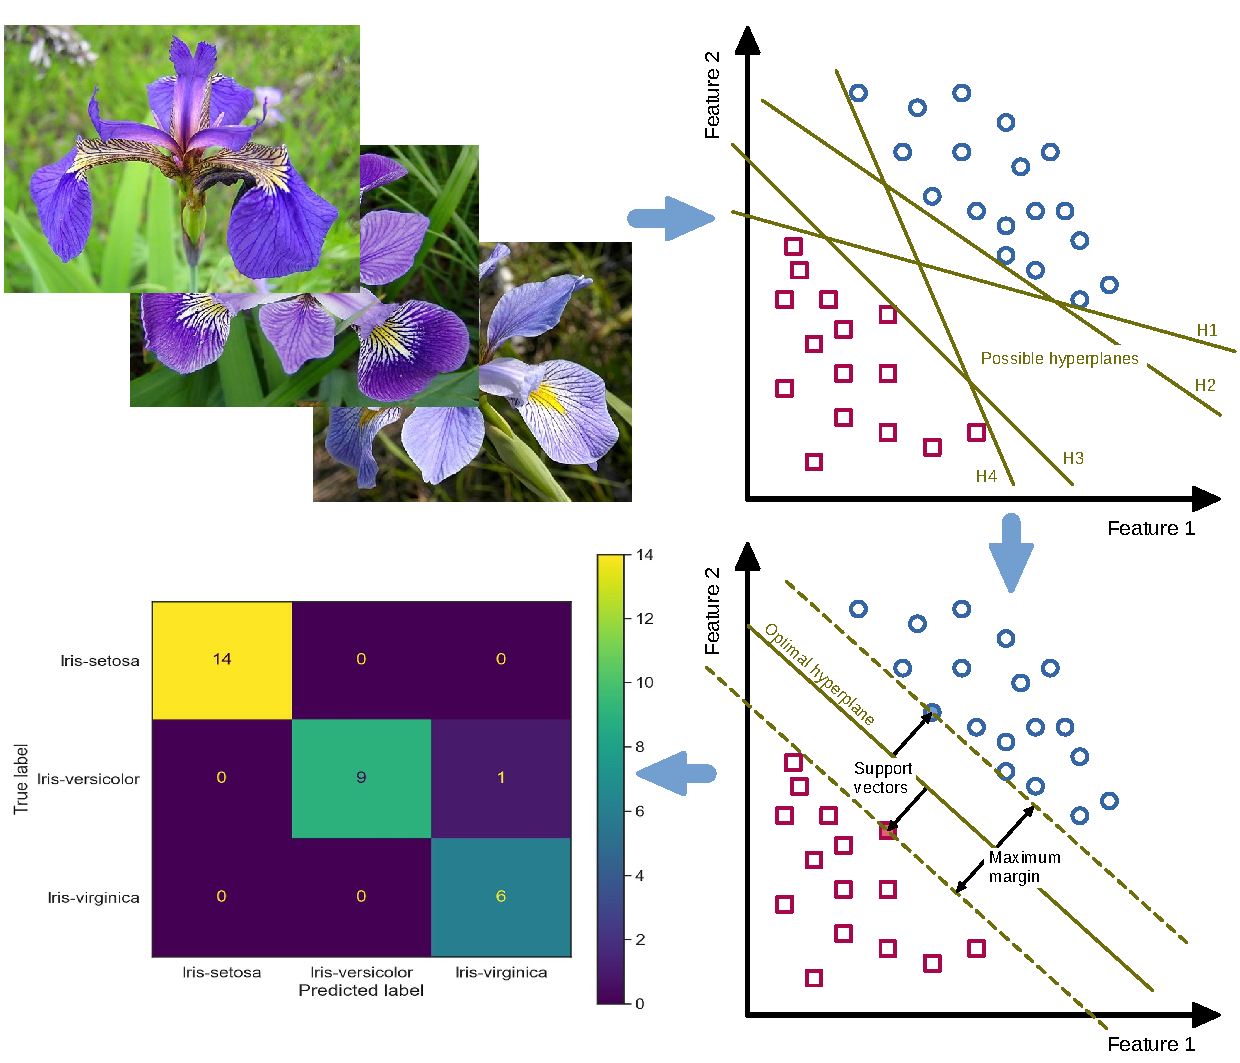
\includegraphics[width=0.90\textwidth]{images/Cover_image.pdf}
        \end{center}
        \vfill

    \begin{abstract}
    Anyone who wants to seriously deal with the hypothetical topic of our time ``Artificial Intelligence (AI)'' or ``Machine Learning (ML)'' cannot avoid dealing with the basic ML algorithms, corresponding software tools, libraries and programming systems. However, someone who opens the door for the first time to this equally very exciting as well as arbitrarily complex and, at first glance, confusing world will very quickly be overwhelmed. Here, it is a good idea to consult introductory and systematic tutorials. Therefore, this Getting Started tutorial systematically demonstrates the typical ML work process step-by-step using the very powerful and performant ``Support Vector Classifier (SVC)'' and the widely known and very beginner-friendly ``Iris Dataset''. Furthermore, the selection of the ``correct'' SVC kernel and its parameters are described and their effect on the classification result is shown.
    \end{abstract}
    \vfill
    
    \noindent
    \begin{tabular}{l l}
    \begin{minipage}{0.24\textwidth}
        
\includegraphics{images/CC_BY-SA_40.png}
    \end{minipage}
    &
    \begin{minipage}{0.68\textwidth}
        This work is licensed under a \href{https://creativecommons.org/licenses/by-sa/4.0/}{Creative Commons Attribution-ShareAlike 4.0 International License (CC BY-SA 4.0)}.
    \end{minipage}
    \end{tabular}

    \newpage

    % Activate own page style
    \pagestyle{fancy}
    % Delete all fields
    \fancyhf{}
    % \fancyhead[EL,OL]{$header$}
    % \fancyfoot[EL,OL]{$footer$}
    % Header leftside: chapter/section
    \fancyhead[ER,OR]{\leftmark}
    % Footer rightside: page number
    \fancyfoot[ER,OR]{Seite \thepage}

    \renewcommand{\sectionmark}[1]{
        \markboth{\thesection{} #1}{}
    }

    
    \tableofcontents
    



    
    \hypertarget{introduction}{%
\section{Introduction}\label{introduction}}

\hypertarget{english-introduction}{%
\subsection{English introduction}\label{english-introduction}}

In the \textbf{digitised work environment}, there is an increasing
demand for \textbf{Work equipment} to be able to adapt independently and
in a task-related manner to changing work situations. This
\textbf{situational adaptivity} can often only be realised through the
use of \textbf{Artificial Intelligence (AI)} or \textbf{Machine Learning
(ML)}, depending on the degree of flexibility. Examples of such AI
applications in the world of work can range from comparatively simple
\textbf{voice assistance systems} (similar, for example, to Siri or
Alexa from the private sphere) to partially or even \textbf{fully
autonomous systems}. Such fully autonomous systems are, for example,
autonomously driving logistics vehicles in larger industrial plants
(so-called \textbf{driverless transport systems}).

In addition to the many very interesting advantages in terms of economic
efficiency, workload reduction, etc., such fully autonomous systems are
characterised by a very high level of technical complexity. This
concerns both their \textbf{operating functions} (e.g.~autonomous
navigation through complex industrial environments with shared use of
the roadways by other human-controlled vehicles) and their
\textbf{safety functions} (e.g.~evaluation of complex, interconnected,
mostly imaging safety sensors for monitoring the driving space).

Very high demands are placed on such autonomous systems and the AI
algorithms used for them with regard to \textbf{functional safety}.
However, when assessing their safety, one quickly comes up against clear
limits with regard to the \textbf{transparency} and
\textbf{explainability} of the decisions made by AI as well as limits to
the \textbf{recognition rates} and thus their \textbf{reliability}. In
particular, the detection rates achievable by AI even under the most
convenient conditions very often do not meet the requirements for
realising higher safety levels (e.g.~Performance Level d (PLd) according
to ISO 13849).

An appropriate assessment or even \textbf{testing} with regard to the
required functional safety according to uniform and ideally standardised
criteria has many implications for the future orientation of technical
\textbf{occupational safety and health (OSH)} in Germany and in Europe.
In addition to the currently still very difficult algorithmic
evaluability, a significant aspect is that the previous clear separation
between \textbf{placing on the market law} (see e.g.~Machinery
Directive) and \textbf{occupational health and safety law} (see European
Occupational Health and Safety Framework Directive and German Ordinance
on Occupational Safety and Health) can no longer be continued in this
way. The reason for this is that the \textbf{safety-relevant properties}
of the autonomous systems will change due to new or \textbf{adapted
behaviours} learned during operation.

For these reasons, those involved in technical occupational safety and
health who will be involved in the testing of work equipment in the
future should deal with AI and ML algorithms in depth as early as
possible. This is the only way to ensure that the rapid development of
adaptive systems capable of learning can be accompanied by OSH and its
testing institutes in a constructive, critical and technically
appropriate manner. If this is not done, the OSH system will be
ruthlessly circumvented or undermined by the economic interests of
globally operating software giants. This would have the consequence that
serious or fatal occupational accidents are likely to occur due to
inadequately designed AI-based work systems.

Anyone seeking a serious technical entrance into the world of
\textbf{Artificial Intelligence (AI)} or \textbf{Machine Learning (ML)}
will not be able to avoid dealing with the basic ML algorithms,
corresponding software tools, libraries and programming systems.

However, someone who opens the door for the first time to this equally
very exciting as well as arbitrarily complex and, at first glance,
confusing world will very quickly be overwhelmed. Here, it is a good
idea to consult introductory and systematic tutorials.

The aim of this Getting Started tutorial is to systematically
demonstrate the typical ML working process step-by-step based on the
example of the very powerful and performant \textbf{Support Vector
Classifier (SVC)}.

This tutorial will be presented as part of a workshop at the DGUV
symposium \textbf{Artificial Intelligence}, probably in November 2022 in
Dresden. The workshop addresses interested ML novices in the technical
occupational safety and health of the social accident insurance
institutions.

For the target audience in the workshop, the SVC algorithm was
intentionally chosen to show that there are many other very powerful and
performant ML algorithms apart from the \textbf{deep neural networks}
that are very present in the media. On the other hand, a necessary and
comprehensible introduction to neural networks and the the technical
background to perceptrons, activation functions etc. for newcomers would
not be possible within the time frame given for the workshop.

Furthermore, this tutorial does \emph{not} address the generation or
acquisition of ML-ready datasets. Reason for this is that a newcomer to
ML will (or should) first try to familiarize himself with ML algorithms,
tools, libraries and programming systems. Only then it makes sense to
explore one's own environment with respect to ML-suitable applications
and to acquire suitable datasets from them.

Therefore, this tutorial demonstrates the usage of selected ML tools in
the form of Python libraries as well as the systematic approach to the
widely known and very beginner-friendly \textbf{Iris dataset}. According
to the literature, the Support Vector Classifier is particularly well
suited for the classification of the iris dataset in terms of
recognition rate and performance. Alternatively, decision tree-based ML
algorithms such as the \textbf{Random Forests Classifier} could be used.

After the classification of the iris dataset by the SVC initially with
standard parameters, the selection of the ``correct'' SVC kernel with
its setting parameters is furthermore described and the effect on the
classification result is shown.

    \hypertarget{german-introduction}{%
\subsection{German introduction}\label{german-introduction}}

Von den \textbf{Arbeitsmitteln} in der \textbf{digitalisierten
Arbeitswelt} wird immer stärker gefordert, dass sie sich selbstständig
und aufgabenbezogen an sich ändernde Arbeitssituationen anpassen können.
Diese \textbf{situative Adaptivität} kann je nach Stärke des
Flexibilisierungsgrades oft nur durch Anwendung von \textbf{Artificial
Intelligence (AI)} oder \textbf{Machine Learning (ML)} realisiert
werden.

Als Beispiele für solche KI-Anwendungen in der Arbeitswelt können
vergleichsweise einfache \textbf{Sprachassistenzsysteme} (ähnlich z. B.
Siri oder Alexa aus dem privaten Umfeld) bis hin zu teil- oder gar
\textbf{vollautonomen Systemen} genannt werden. Solche vollautonomen
Systemen sind beispielsweise autonom fahrende Logistikfahrzeuge in
größeren Industrieanlagen (sog. \textbf{fahrerlosen Transportsystemen}).

Neben den vielen sehr interessanten Vorteilen bzgl. Wirtschaftlichkeit,
Arbeitserleichterung usw. kennzeichnet solche vollautonomen Systeme eine
sehr hohe technische Komplexität. Diese betrifft sowohl ihre
\textbf{Betriebsfunktionen} (z. B. autonome Navigation durch komplexe
industrielle Umgebungen bei gemeinsamer Nutzung der Fahrwege durch
andere menschlich gesteuerte Fahrzeuge) als auch seiner
\textbf{Sicherheitsfunktionen} (z. B. Auswertung komplexer, miteinander
verknüpfter, meist bildgebender Sicherheitssensorik zur Überwachung des
Fahrraums).

An solche autonomen Systeme und die hierfür eingesetzten KI-Algorithmen
werden sehr hohe Anforderungen hinsichtlich der \textbf{funktionalen
Sicherheit} gestellt. Jedoch stößt man bei ihrer sicherheitstechnischen
Bewertung heute noch sehr schnell an deutliche Grenzen hinsichtlich der
\textbf{Transparenz} und \textbf{Erklärbarkeit} der durch KI getroffenen
Entscheidungen sowie Grenzen der \textbf{Erkennnungsraten} und damit
ihrer \textbf{Zuverlässigkeit}. Insbesondere erfüllen die durch KI
selbst unter günstigsten Bedingungen erreichbaren Erkennnungsraten sehr
oft nicht die Anforderderungen, um höhere Safety-Level (z. B.
Performance Level d (PLd) nach ISO 13849) zu realisieren.

Eine hinsichtlich der geforderten funktionalen Sicherheit angemessene
Bewertung oder gar \textbf{Prüfung} nach einheitlichen und idealerweise
genormten Maßstäben hat viele Implikationen auf die zukünftige
Ausrichtung des \textbf{technischen Arbeitsschutzes} in Deutschland und
in Europa. Neben der derzeit noch sehr schwierigen algorithmischen
Bewertbarkeit ist ein wesentlicher Aspekt, dass die bisherige klare
Trennung zwischen \textbf{Inverkehrbringensrecht} (siehe z. B.
Maschinenrichtlinie) und \textbf{betrieblichem Arbeitsschutzrecht}
(siehe Arbeitschutzrahmenrichtlinie und Betriebssicherheitsverordnung)
so nicht mehr aufrechterhalten werden kann. Grund hierfür ist, dass sich
die \textbf{sicherheitsrelevanten Eigenschaften} der autonomen Systeme
durch während des Betriebs erlernte, neue oder \textbf{angepasste
Verhaltensweisen} verändern werden.

Aus diesen Gründen sollten sich insbesondere die zukünftig mit der
Prüfung befassten Akteure des technischen Arbeitsschutzes möglichst
frühzeitig mit den KI- bzw. ML-Algorithmen vertieft auseinandersetzen.
Nur dadurch lässt sich erreichen, dass die stürmische Entwicklung
lernfähiger, adaptiver Systeme durch den Arbeitsschutz und deren
Prüfinstitute konstruktiv, kritisch und fachlich angemessen begleitet
werden kann. Wird dies versäumt, wird das Arbeitsschutzsystem durch die
wirtschaftlichen Interessen global agierender Softwaregiganten
skrupellos umgangen oder ausgehebelt werden. Dies hätte die Folge, dass
schwere oder tödliche Arbeitsunfälle auf Grund unzulänglich gestalteter
KI-basierter Arbeitssysteme wahrscheinlich werden.

Wer einen ernsthaften fachlichen Einstieg in die Welt von
\textbf{Künstlicher Intelligenz (KI)} bzw. \textbf{Machine Learning
(ML)} sucht, wird nicht umhin kommen, sich mit den grundlegenden
ML-Algorithmen, entsprechenden Software-Werkzeugen, Bibliotheken und
Programmiersystemen auseinander zu setzen.

Wer jedoch zum ersten Mal die Tür zu dieser ebenso spannenden wie
beliebig komplexen und auf den ersten Blick verwirrenden Welt öffnet,
wird sehr schnell überfordert sein. Hier empfiehlt es sich, einführende
und systematische Anleitungen zu Rate zu ziehen.

Ziel dieses Getting-Started-Tutorials ist es, den typischen
ML-Arbeitsablauf systematisch und Schritt-für-Schritt am Beispiel des
sehr leistungsfähigen \textbf{Support Vector Classifier (SVC)} zu
demonstrieren.

Dieses Tutorial wird im Rahmen eines Workshops auf der DGUV-Fachtagung
\textbf{Künstliche Intelligenz} voraussichtlich im November 2022 in
Dresden vorgestellt. Der Workshop richtet sich an interessierte
ML-Neulinge im technischen Arbeitsschutz der gesetzlichen
Unfallversicherungsträger.

Für die Zielgruppe des Workshops wurde der SVC-Algorithmus bewusst
gewählt, um zu zeigen, dass es neben den \textbf{tiefen neuronalen
Netzen}, die in den Medien sehr präsent sind, noch viele andere sehr
leistungsfähige ML-Algorithmen gibt. Andererseits wäre eine notwendige
und verständliche Einführung in neuronale Netze und die technischen
Hintergründe zu Perzeptronen, Aktivierungsfunktionen etc. für Neulinge
in dem für den Workshop vorgegebenen Zeitrahmen nicht möglich gewesen.

Außerdem befasst sich dieses Tutorial \emph{nicht} mit der Erzeugung
oder Akquisition von ML-tauglichen Datensätzen. Der Grund dafür ist,
dass ein ML-Neuling zunächst versuchen wird (oder sollte), sich mit den
ML-Algorithmen, Werkzeugen, Bibliotheken und Programmiersystemen
vertraut zu machen. Erst dann ist es sinnvoll, die eigene Umgebung auf
ML-taugliche Anwendungen hin zu untersuchen und daraus geeignete
Datensätze zu gewinnen.

Daher demonstriert dieses Tutorial die Verwendung ausgewählter ML-Tools
in Form von Python-Bibliotheken sowie die systematische Herangehensweise
an den weithin bekannten und sehr einsteigerfreundlichen
\textbf{Iris-Datensatz}. Laut Fachliteratur ist für die Klassifikation
des Iris-Datensatzes der Support Vector Classifier hinsichtlich
Erkennungsrate als auch Performanz besonders gut geeignet. Alternativ
könnten auch entscheidungsbaum-basierte ML-Algorithmen wie z. B. der
\textbf{Random-forests-Klassifikator} eingesetzt werden.

Nach der Klassifikation des Iris-Datensatzes durch den SVC zunächst mit
Standard-Parametern wird darüber hinaus die Auswahl des ``richtigen''
SVC-Kernels mit seinen Einstellparametern beschrieben und die Auswirkung
auf das Klassifikationsergebnis wird gezeigt.

    \hypertarget{steps-of-the-systematic-ml-process}{%
\subsection{Steps of the systematic ML
process}\label{steps-of-the-systematic-ml-process}}

The following steps of the systematic ML process are covered in the next
main sections:

\begin{itemize}
\tightlist
\item
  \hyperref[step-0-get-the-dataset]{STEP 0: Get the dataset}
\item
  \hyperref[step-1-exploring-the-dataset]{STEP 1: Exploring the dataset}
\item
  \hyperref[step-2-prepare-the-dataset]{STEP 2: Prepare the dataset}
\item
  \hyperref[step-3-classify-by-support-vector-classifier---svc]{STEP 3: Classify by support vector classifier - SVC}
\item
  \hyperref[step-4-evaluate-the-classification-results---metrics]{STEP 4: Evaluate the classification results - metrics}
\item
  \hyperref[step-5-select-svc-kernel-and-vary-parameters]{STEP 5: Select SVC kernel and vary parameters}
\end{itemize}

    \hypertarget{load-globally-used-libraries-and-set-plot-parameters}{%
\section{Load globally used libraries and set plot
parameters}\label{load-globally-used-libraries-and-set-plot-parameters}}

    \begin{tcolorbox}[breakable, size=fbox, boxrule=1pt, pad at break*=1mm,colback=cellbackground, colframe=cellborder]
\prompt{In}{incolor}{1}{\boxspacing}
\begin{Verbatim}[commandchars=\\\{\}]
\PY{k+kn}{import} \PY{n+nn}{time}

\PY{k+kn}{from} \PY{n+nn}{IPython}\PY{n+nn}{.}\PY{n+nn}{display} \PY{k+kn}{import} \PY{n}{HTML}

\PY{k+kn}{import} \PY{n+nn}{pandas} \PY{k}{as} \PY{n+nn}{pd}
\PY{k+kn}{import} \PY{n+nn}{matplotlib}\PY{n+nn}{.}\PY{n+nn}{pyplot} \PY{k}{as} \PY{n+nn}{plt}
\PY{k+kn}{from} \PY{n+nn}{sklearn} \PY{k+kn}{import} \PY{n}{svm}\PY{p}{,} \PY{n}{metrics}
\PY{k+kn}{import} \PY{n+nn}{seaborn} \PY{k}{as} \PY{n+nn}{sns}
\PY{o}{\PYZpc{}}\PY{k}{matplotlib} inline
\end{Verbatim}
\end{tcolorbox}

    \hypertarget{step-0-get-the-dataset}{%
\section{STEP 0: Get the dataset}\label{step-0-get-the-dataset}}

Since this is intended to be an introduction to the world of machine
learning (ML), this step does NOT deal with the design of an application
suitable for ML and the acquisition of valid measurement data.

In order to get to know the typical work steps and ML tools, the use of
\textbf{well-known and well-researched data sets} is clearly
\textbf{recommended}.

In the further course, the famous
\href{https://en.wikipedia.org/wiki/Iris_flower_data_set}{Iris flower
data sets} will be used. It can be downloaded on
\href{https://www.kaggle.com/datasets/arshid/iris-flower-dataset}{Iris
Flower Dataset \textbar{} Kaggle}. Furthermore, the dataset is included
in Python in the machine learning package
\href{https://scikit-learn.org}{Scikit-learn}, so that users can access
it without having to find a special source for it.

    \begin{tcolorbox}[breakable, size=fbox, boxrule=1pt, pad at break*=1mm,colback=cellbackground, colframe=cellborder]
\prompt{In}{incolor}{2}{\boxspacing}
\begin{Verbatim}[commandchars=\\\{\}]
\PY{c+c1}{\PYZsh{} import some data to play with}
\PY{n}{irisdata\PYZus{}df} \PY{o}{=} \PY{n}{pd}\PY{o}{.}\PY{n}{read\PYZus{}csv}\PY{p}{(}\PY{l+s+s1}{\PYZsq{}}\PY{l+s+s1}{./datasets/IRIS\PYZus{}flower\PYZus{}dataset\PYZus{}kaggle.csv}\PY{l+s+s1}{\PYZsq{}}\PY{p}{)}
\end{Verbatim}
\end{tcolorbox}

    \hypertarget{step-1-exploring-the-dataset}{%
\section{STEP 1: Exploring the
dataset}\label{step-1-exploring-the-dataset}}

\hypertarget{goals-of-exploration}{%
\subsection{Goals of exploration}\label{goals-of-exploration}}

The objectives of the exploration of the dataset are as follows:

\begin{enumerate}
\def\labelenumi{\arabic{enumi}.}
\tightlist
\item
  Clarify the \textbf{origins history}:

  \begin{itemize}
  \tightlist
  \item
    Where did the data come from? =\textgreater{} Contact persons and
    licensing permissions?
  \item
    Who obtained the data and with which (measurement) methods?
    =\textgreater{} Did systematic errors occur during the acquisition?
  \item
    What were they originally intended for? =\textgreater{} Can they be
    used for my application?
  \end{itemize}
\item
  Overview of the internal \textbf{structure and organisation} of the
  data:

  \begin{itemize}
  \tightlist
  \item
    Which columns are there? =\textgreater{} With which methods can they
    be read in (e.g.~import of CSV files)?
  \item
    What do they contain for (physical) measured variables?
    =\textgreater{} Which technical or physical correlations exist?
  \item
    Which data formats or types are there? =\textgreater{} Do they have
    to be converted?
  \item
    In which value ranges do the measurement data vary? =\textgreater{}
    Are normalizations necessary?
  \end{itemize}
\item
  Identify \textbf{anomalies} in the data sets:

  \begin{itemize}
  \tightlist
  \item
    Do the data have \textbf{gaps} or \textbf{duplicates}?
    =\textgreater{} Does the data set needs to be cleaned?
  \item
    Are there obvious erroneous entries or measurement outliers?
    =\textgreater{} Does (statistical) filtering have to be carried out?
  \end{itemize}
\item
  Avoidance of \textbf{tendencies due to bias}:

  \begin{itemize}
  \tightlist
  \item
    Are all possible classes included in the dataset and equally
    distributed? =\textgreater{} Does the data set need to be enriched
    with additional data for balance?
  \end{itemize}
\item
  Find a first rough \textbf{idea of which correlations} could be in the
  data set
\end{enumerate}

    \hypertarget{clarify-the-origins-history}{%
\subsection{\texorpdfstring{Clarify the \textbf{origins
history}}{Clarify the origins history}}\label{clarify-the-origins-history}}

\begin{quote}
The \textbf{\emph{Iris} flower data sets} is a multivariate data set
introduced by the British statistician and biologist \emph{Ronald
Fisher} in his paper ``The use of multiple measurements in taxonomic
problems as an example of linear discriminant analysis'' (1936). It is
sometimes called \emph{Anderson's Iris data set} because Edgar Anderson
collected the data to quantify the morphologic variation of Iris flowers
of three related species (source:
\href{https://en.wikipedia.org/w/index.php?title=Iris_flower_data_set\&oldid=1090001619}{Iris
flower data set}).
\end{quote}

The dataset is published in Public Domain with a
\href{https://creativecommons.org/share-your-work/public-domain/cc0/}{CC0-License}.

This dataset became a typical test case for many statistical
classification techniques in machine learning such as \textbf{support
vector machines}.

\begin{quote}
{[}..{]} measurements of the flowers of fifty plants each of the two
species \emph{Iris setosa} and \emph{I. versicolor}, found
\textbf{growing together in the same colony} and measured by Dr E.
Anderson {[}..{]} (source: R. A. Fisher (1936). ``The use of multiple
measurements in taxonomic problems''.
\href{https://onlinelibrary.wiley.com/doi/10.1111/j.1469-1809.1936.tb02137.x}{Annals
of Eugenics})
\end{quote}

\begin{quote}
{[}..{]} \emph{Iris virginica}, differs from the two other samples in
\textbf{not being taken from the same natural colony} {[}..{]} (source:
ibidem)
\end{quote}

    \hypertarget{overview-of-the-internal-structure-and-organisation-of-the-data}{%
\subsection{\texorpdfstring{Overview of the internal \textbf{structure
and organisation} of the
data}{Overview of the internal structure and organisation of the data}}\label{overview-of-the-internal-structure-and-organisation-of-the-data}}

The data set consists of 50 samples from each of three species of Iris
(\href{https://en.wikipedia.org/wiki/Iris_setosa}{\emph{Iris setosa}},
\href{https://en.wikipedia.org/wiki/Iris_virginica}{\emph{Iris
virginica}} and
\href{https://en.wikipedia.org/wiki/Iris_versicolor}{\emph{Iris
versicolor}}), so there are 150 total samples. Four features were
measured from each sample: the length and the width of the
\href{https://en.wikipedia.org/wiki/Sepal}{sepals} and
\href{https://en.wikipedia.org/wiki/Petal}{petals}, in centimetres.\\
Here is a principle illustration of a flower with sepal and petal:

    \begin{figure}
\centering
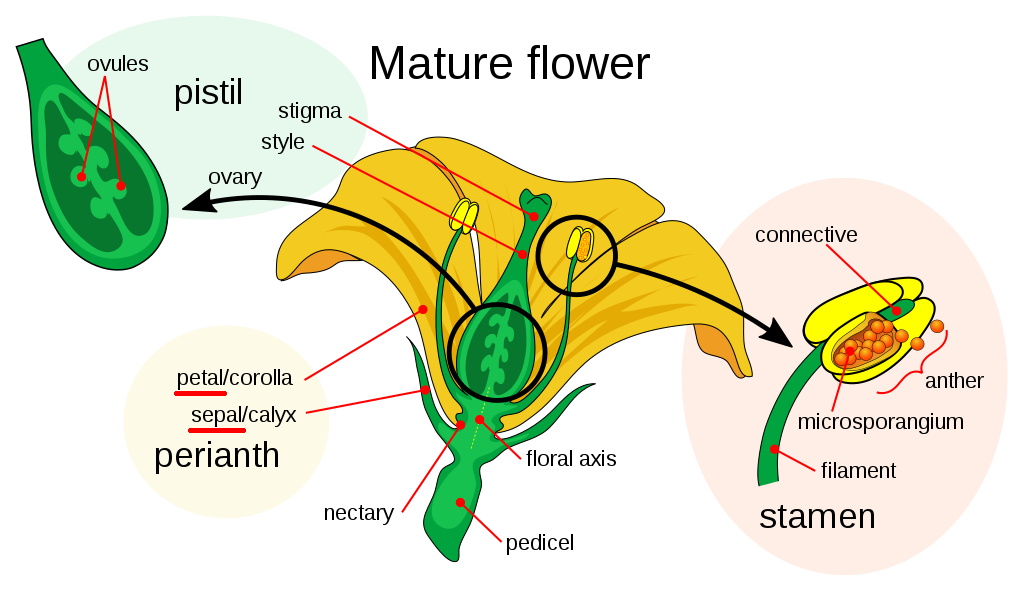
\includegraphics{images/Mature_flower_diagram_1024px.png}
\caption{Principle illustration of a flower with sepal and petal
(source:
\href{https://en.wikipedia.org/wiki/File:Mature_flower_diagram.svg}{Mature\_flower\_diagram.svg},
license: public domain)}
\end{figure}

    Here are pictures of the three different Iris species (\emph{Iris
setosa}, \emph{Iris virginica} and \emph{Iris versicolor}). Given the
dimensions of the flower, it will be possible to predict the class of
the flower.

    \begin{figure}
\centering
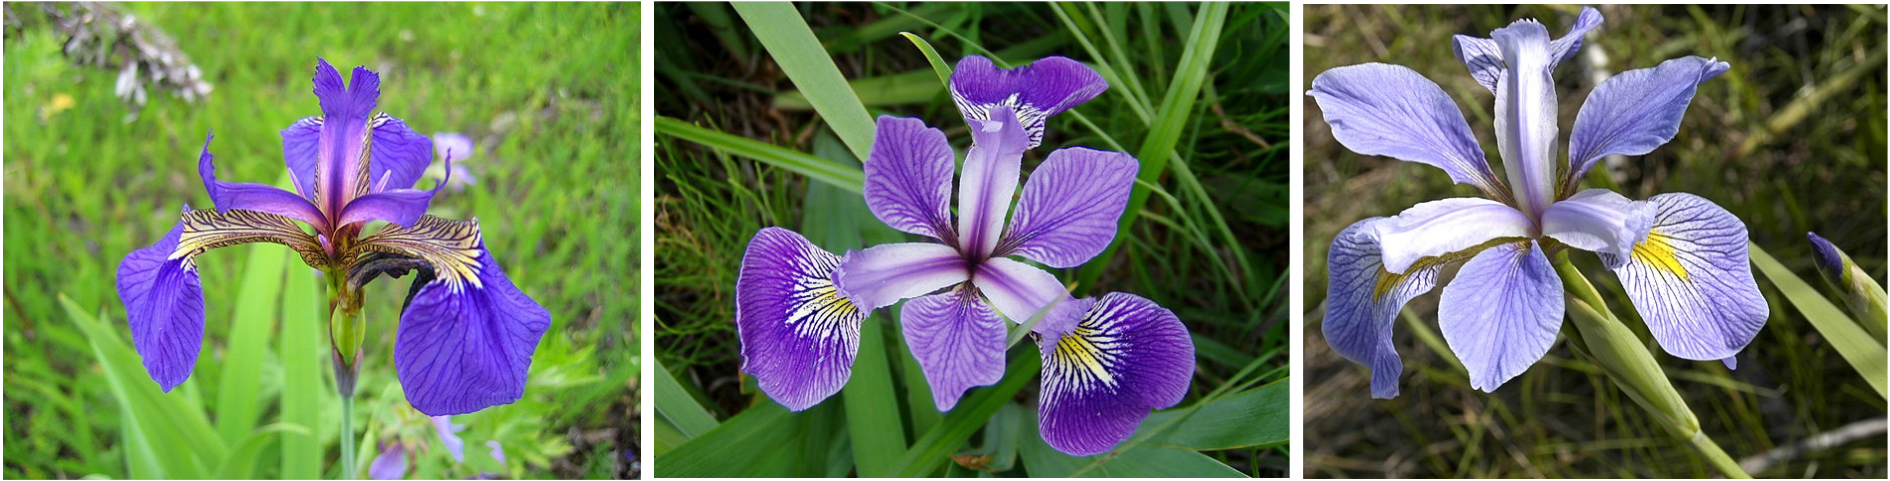
\includegraphics{images/Iris_images.png}
\caption{left: \emph{Iris setosa} (source:
\href{https://commons.wikimedia.org/wiki/File:Irissetosa1.jpg}{Irissetosa1.jpg},
license: public domain); middle: \emph{Iris versicolor} (source:
\href{https://en.wikipedia.org/wiki/File:Iris_versicolor_3.jpg}{Iris\_versicolor\_3.jpg},
license: CC-SA 3.0); right: \emph{Iris virginica} (source:
\href{https://en.wikipedia.org/wiki/File:Iris_virginica.jpg}{Iris\_virginica.jpg},
license: CC-SA 2.0)}
\end{figure}

    \hypertarget{inspect-structure-of-dataframe}{%
\subsubsection{\texorpdfstring{Inspect \textbf{structure of
dataframe}}{Inspect structure of dataframe}}\label{inspect-structure-of-dataframe}}

Print first or last 5 rows of dataframe:

    \begin{tcolorbox}[breakable, size=fbox, boxrule=1pt, pad at break*=1mm,colback=cellbackground, colframe=cellborder]
\prompt{In}{incolor}{3}{\boxspacing}
\begin{Verbatim}[commandchars=\\\{\}]
\PY{n}{irisdata\PYZus{}df}\PY{o}{.}\PY{n}{head}\PY{p}{(}\PY{p}{)}
\end{Verbatim}
\end{tcolorbox}

            \begin{tcolorbox}[breakable, size=fbox, boxrule=.5pt, pad at break*=1mm, opacityfill=0]
\prompt{Out}{outcolor}{3}{\boxspacing}
\begin{Verbatim}[commandchars=\\\{\}]
   sepal\_length  sepal\_width  petal\_length  petal\_width      species
0           5.1          3.5           1.4          0.2  Iris-setosa
1           4.9          3.0           1.4          0.2  Iris-setosa
2           4.7          3.2           1.3          0.2  Iris-setosa
3           4.6          3.1           1.5          0.2  Iris-setosa
4           5.0          3.6           1.4          0.2  Iris-setosa
\end{Verbatim}
\end{tcolorbox}
        
    \begin{tcolorbox}[breakable, size=fbox, boxrule=1pt, pad at break*=1mm,colback=cellbackground, colframe=cellborder]
\prompt{In}{incolor}{4}{\boxspacing}
\begin{Verbatim}[commandchars=\\\{\}]
\PY{n}{irisdata\PYZus{}df}\PY{o}{.}\PY{n}{tail}\PY{p}{(}\PY{p}{)}
\end{Verbatim}
\end{tcolorbox}

            \begin{tcolorbox}[breakable, size=fbox, boxrule=.5pt, pad at break*=1mm, opacityfill=0]
\prompt{Out}{outcolor}{4}{\boxspacing}
\begin{Verbatim}[commandchars=\\\{\}]
     sepal\_length  sepal\_width  petal\_length  petal\_width         species
145           6.7          3.0           5.2          2.3  Iris-virginica
146           6.3          2.5           5.0          1.9  Iris-virginica
147           6.5          3.0           5.2          2.0  Iris-virginica
148           6.2          3.4           5.4          2.3  Iris-virginica
149           5.9          3.0           5.1          1.8  Iris-virginica
\end{Verbatim}
\end{tcolorbox}
        
    While printing a dataframe - only an abbreviated view of the dataframe
is shown :(\\
Default setting in the pandas library makes it to display only 5 lines
from head and from tail.

    \begin{tcolorbox}[breakable, size=fbox, boxrule=1pt, pad at break*=1mm,colback=cellbackground, colframe=cellborder]
\prompt{In}{incolor}{5}{\boxspacing}
\begin{Verbatim}[commandchars=\\\{\}]
\PY{n}{irisdata\PYZus{}df}
\end{Verbatim}
\end{tcolorbox}

            \begin{tcolorbox}[breakable, size=fbox, boxrule=.5pt, pad at break*=1mm, opacityfill=0]
\prompt{Out}{outcolor}{5}{\boxspacing}
\begin{Verbatim}[commandchars=\\\{\}]
     sepal\_length  sepal\_width  petal\_length  petal\_width         species
0             5.1          3.5           1.4          0.2     Iris-setosa
1             4.9          3.0           1.4          0.2     Iris-setosa
2             4.7          3.2           1.3          0.2     Iris-setosa
3             4.6          3.1           1.5          0.2     Iris-setosa
4             5.0          3.6           1.4          0.2     Iris-setosa
..            {\ldots}          {\ldots}           {\ldots}          {\ldots}             {\ldots}
145           6.7          3.0           5.2          2.3  Iris-virginica
146           6.3          2.5           5.0          1.9  Iris-virginica
147           6.5          3.0           5.2          2.0  Iris-virginica
148           6.2          3.4           5.4          2.3  Iris-virginica
149           5.9          3.0           5.1          1.8  Iris-virginica

[150 rows x 5 columns]
\end{Verbatim}
\end{tcolorbox}
        
    To print all rows of a dataframe, the option \texttt{display.max\_rows}
has to set to \texttt{None} in pandas:

    \begin{tcolorbox}[breakable, size=fbox, boxrule=1pt, pad at break*=1mm,colback=cellbackground, colframe=cellborder]
\prompt{In}{incolor}{6}{\boxspacing}
\begin{Verbatim}[commandchars=\\\{\}]
\PY{n}{pd}\PY{o}{.}\PY{n}{set\PYZus{}option}\PY{p}{(}\PY{l+s+s1}{\PYZsq{}}\PY{l+s+s1}{display.max\PYZus{}rows}\PY{l+s+s1}{\PYZsq{}}\PY{p}{,} \PY{k+kc}{None}\PY{p}{)}
\PY{n}{irisdata\PYZus{}df}
\end{Verbatim}
\end{tcolorbox}

            \begin{tcolorbox}[breakable, size=fbox, boxrule=.5pt, pad at break*=1mm, opacityfill=0]
\prompt{Out}{outcolor}{6}{\boxspacing}
\begin{Verbatim}[commandchars=\\\{\}]
     sepal\_length  sepal\_width  petal\_length  petal\_width          species
0             5.1          3.5           1.4          0.2      Iris-setosa
1             4.9          3.0           1.4          0.2      Iris-setosa
2             4.7          3.2           1.3          0.2      Iris-setosa
3             4.6          3.1           1.5          0.2      Iris-setosa
4             5.0          3.6           1.4          0.2      Iris-setosa
5             5.4          3.9           1.7          0.4      Iris-setosa
6             4.6          3.4           1.4          0.3      Iris-setosa
7             5.0          3.4           1.5          0.2      Iris-setosa
8             4.4          2.9           1.4          0.2      Iris-setosa
9             4.9          3.1           1.5          0.1      Iris-setosa
10            5.4          3.7           1.5          0.2      Iris-setosa
11            4.8          3.4           1.6          0.2      Iris-setosa
12            4.8          3.0           1.4          0.1      Iris-setosa
13            4.3          3.0           1.1          0.1      Iris-setosa
14            5.8          4.0           1.2          0.2      Iris-setosa
15            5.7          4.4           1.5          0.4      Iris-setosa
16            5.4          3.9           1.3          0.4      Iris-setosa
17            5.1          3.5           1.4          0.3      Iris-setosa
18            5.7          3.8           1.7          0.3      Iris-setosa
19            5.1          3.8           1.5          0.3      Iris-setosa
20            5.4          3.4           1.7          0.2      Iris-setosa
21            5.1          3.7           1.5          0.4      Iris-setosa
22            4.6          3.6           1.0          0.2      Iris-setosa
23            5.1          3.3           1.7          0.5      Iris-setosa
24            4.8          3.4           1.9          0.2      Iris-setosa
25            5.0          3.0           1.6          0.2      Iris-setosa
26            5.0          3.4           1.6          0.4      Iris-setosa
27            5.2          3.5           1.5          0.2      Iris-setosa
28            5.2          3.4           1.4          0.2      Iris-setosa
29            4.7          3.2           1.6          0.2      Iris-setosa
30            4.8          3.1           1.6          0.2      Iris-setosa
31            5.4          3.4           1.5          0.4      Iris-setosa
32            5.2          4.1           1.5          0.1      Iris-setosa
33            5.5          4.2           1.4          0.2      Iris-setosa
34            4.9          3.1           1.5          0.1      Iris-setosa
35            5.0          3.2           1.2          0.2      Iris-setosa
36            5.5          3.5           1.3          0.2      Iris-setosa
37            4.9          3.1           1.5          0.1      Iris-setosa
38            4.4          3.0           1.3          0.2      Iris-setosa
39            5.1          3.4           1.5          0.2      Iris-setosa
40            5.0          3.5           1.3          0.3      Iris-setosa
41            4.5          2.3           1.3          0.3      Iris-setosa
42            4.4          3.2           1.3          0.2      Iris-setosa
43            5.0          3.5           1.6          0.6      Iris-setosa
44            5.1          3.8           1.9          0.4      Iris-setosa
45            4.8          3.0           1.4          0.3      Iris-setosa
46            5.1          3.8           1.6          0.2      Iris-setosa
47            4.6          3.2           1.4          0.2      Iris-setosa
48            5.3          3.7           1.5          0.2      Iris-setosa
49            5.0          3.3           1.4          0.2      Iris-setosa
50            7.0          3.2           4.7          1.4  Iris-versicolor
51            6.4          3.2           4.5          1.5  Iris-versicolor
52            6.9          3.1           4.9          1.5  Iris-versicolor
53            5.5          2.3           4.0          1.3  Iris-versicolor
54            6.5          2.8           4.6          1.5  Iris-versicolor
55            5.7          2.8           4.5          1.3  Iris-versicolor
56            6.3          3.3           4.7          1.6  Iris-versicolor
57            4.9          2.4           3.3          1.0  Iris-versicolor
58            6.6          2.9           4.6          1.3  Iris-versicolor
59            5.2          2.7           3.9          1.4  Iris-versicolor
60            5.0          2.0           3.5          1.0  Iris-versicolor
61            5.9          3.0           4.2          1.5  Iris-versicolor
62            6.0          2.2           4.0          1.0  Iris-versicolor
63            6.1          2.9           4.7          1.4  Iris-versicolor
64            5.6          2.9           3.6          1.3  Iris-versicolor
65            6.7          3.1           4.4          1.4  Iris-versicolor
66            5.6          3.0           4.5          1.5  Iris-versicolor
67            5.8          2.7           4.1          1.0  Iris-versicolor
68            6.2          2.2           4.5          1.5  Iris-versicolor
69            5.6          2.5           3.9          1.1  Iris-versicolor
70            5.9          3.2           4.8          1.8  Iris-versicolor
71            6.1          2.8           4.0          1.3  Iris-versicolor
72            6.3          2.5           4.9          1.5  Iris-versicolor
73            6.1          2.8           4.7          1.2  Iris-versicolor
74            6.4          2.9           4.3          1.3  Iris-versicolor
75            6.6          3.0           4.4          1.4  Iris-versicolor
76            6.8          2.8           4.8          1.4  Iris-versicolor
77            6.7          3.0           5.0          1.7  Iris-versicolor
78            6.0          2.9           4.5          1.5  Iris-versicolor
79            5.7          2.6           3.5          1.0  Iris-versicolor
80            5.5          2.4           3.8          1.1  Iris-versicolor
81            5.5          2.4           3.7          1.0  Iris-versicolor
82            5.8          2.7           3.9          1.2  Iris-versicolor
83            6.0          2.7           5.1          1.6  Iris-versicolor
84            5.4          3.0           4.5          1.5  Iris-versicolor
85            6.0          3.4           4.5          1.6  Iris-versicolor
86            6.7          3.1           4.7          1.5  Iris-versicolor
87            6.3          2.3           4.4          1.3  Iris-versicolor
88            5.6          3.0           4.1          1.3  Iris-versicolor
89            5.5          2.5           4.0          1.3  Iris-versicolor
90            5.5          2.6           4.4          1.2  Iris-versicolor
91            6.1          3.0           4.6          1.4  Iris-versicolor
92            5.8          2.6           4.0          1.2  Iris-versicolor
93            5.0          2.3           3.3          1.0  Iris-versicolor
94            5.6          2.7           4.2          1.3  Iris-versicolor
95            5.7          3.0           4.2          1.2  Iris-versicolor
96            5.7          2.9           4.2          1.3  Iris-versicolor
97            6.2          2.9           4.3          1.3  Iris-versicolor
98            5.1          2.5           3.0          1.1  Iris-versicolor
99            5.7          2.8           4.1          1.3  Iris-versicolor
100           6.3          3.3           6.0          2.5   Iris-virginica
101           5.8          2.7           5.1          1.9   Iris-virginica
102           7.1          3.0           5.9          2.1   Iris-virginica
103           6.3          2.9           5.6          1.8   Iris-virginica
104           6.5          3.0           5.8          2.2   Iris-virginica
105           7.6          3.0           6.6          2.1   Iris-virginica
106           4.9          2.5           4.5          1.7   Iris-virginica
107           7.3          2.9           6.3          1.8   Iris-virginica
108           6.7          2.5           5.8          1.8   Iris-virginica
109           7.2          3.6           6.1          2.5   Iris-virginica
110           6.5          3.2           5.1          2.0   Iris-virginica
111           6.4          2.7           5.3          1.9   Iris-virginica
112           6.8          3.0           5.5          2.1   Iris-virginica
113           5.7          2.5           5.0          2.0   Iris-virginica
114           5.8          2.8           5.1          2.4   Iris-virginica
115           6.4          3.2           5.3          2.3   Iris-virginica
116           6.5          3.0           5.5          1.8   Iris-virginica
117           7.7          3.8           6.7          2.2   Iris-virginica
118           7.7          2.6           6.9          2.3   Iris-virginica
119           6.0          2.2           5.0          1.5   Iris-virginica
120           6.9          3.2           5.7          2.3   Iris-virginica
121           5.6          2.8           4.9          2.0   Iris-virginica
122           7.7          2.8           6.7          2.0   Iris-virginica
123           6.3          2.7           4.9          1.8   Iris-virginica
124           6.7          3.3           5.7          2.1   Iris-virginica
125           7.2          3.2           6.0          1.8   Iris-virginica
126           6.2          2.8           4.8          1.8   Iris-virginica
127           6.1          3.0           4.9          1.8   Iris-virginica
128           6.4          2.8           5.6          2.1   Iris-virginica
129           7.2          3.0           5.8          1.6   Iris-virginica
130           7.4          2.8           6.1          1.9   Iris-virginica
131           7.9          3.8           6.4          2.0   Iris-virginica
132           6.4          2.8           5.6          2.2   Iris-virginica
133           6.3          2.8           5.1          1.5   Iris-virginica
134           6.1          2.6           5.6          1.4   Iris-virginica
135           7.7          3.0           6.1          2.3   Iris-virginica
136           6.3          3.4           5.6          2.4   Iris-virginica
137           6.4          3.1           5.5          1.8   Iris-virginica
138           6.0          3.0           4.8          1.8   Iris-virginica
139           6.9          3.1           5.4          2.1   Iris-virginica
140           6.7          3.1           5.6          2.4   Iris-virginica
141           6.9          3.1           5.1          2.3   Iris-virginica
142           5.8          2.7           5.1          1.9   Iris-virginica
143           6.8          3.2           5.9          2.3   Iris-virginica
144           6.7          3.3           5.7          2.5   Iris-virginica
145           6.7          3.0           5.2          2.3   Iris-virginica
146           6.3          2.5           5.0          1.9   Iris-virginica
147           6.5          3.0           5.2          2.0   Iris-virginica
148           6.2          3.4           5.4          2.3   Iris-virginica
149           5.9          3.0           5.1          1.8   Iris-virginica
\end{Verbatim}
\end{tcolorbox}
        
    \hypertarget{get-data-types}{%
\subsubsection{Get data types}\label{get-data-types}}

    \begin{tcolorbox}[breakable, size=fbox, boxrule=1pt, pad at break*=1mm,colback=cellbackground, colframe=cellborder]
\prompt{In}{incolor}{7}{\boxspacing}
\begin{Verbatim}[commandchars=\\\{\}]
\PY{n}{irisdata\PYZus{}df}\PY{o}{.}\PY{n}{info}\PY{p}{(}\PY{p}{)}
\end{Verbatim}
\end{tcolorbox}

    \begin{Verbatim}[commandchars=\\\{\}]
<class 'pandas.core.frame.DataFrame'>
RangeIndex: 150 entries, 0 to 149
Data columns (total 5 columns):
 \#   Column        Non-Null Count  Dtype
---  ------        --------------  -----
 0   sepal\_length  150 non-null    float64
 1   sepal\_width   150 non-null    float64
 2   petal\_length  150 non-null    float64
 3   petal\_width   150 non-null    float64
 4   species       150 non-null    object
dtypes: float64(4), object(1)
memory usage: 6.0+ KB
    \end{Verbatim}

    \begin{tcolorbox}[breakable, size=fbox, boxrule=1pt, pad at break*=1mm,colback=cellbackground, colframe=cellborder]
\prompt{In}{incolor}{8}{\boxspacing}
\begin{Verbatim}[commandchars=\\\{\}]
\PY{n}{irisdata\PYZus{}df}\PY{o}{.}\PY{n}{describe}\PY{p}{(}\PY{p}{)}
\end{Verbatim}
\end{tcolorbox}

            \begin{tcolorbox}[breakable, size=fbox, boxrule=.5pt, pad at break*=1mm, opacityfill=0]
\prompt{Out}{outcolor}{8}{\boxspacing}
\begin{Verbatim}[commandchars=\\\{\}]
       sepal\_length  sepal\_width  petal\_length  petal\_width
count    150.000000   150.000000    150.000000   150.000000
mean       5.843333     3.054000      3.758667     1.198667
std        0.828066     0.433594      1.764420     0.763161
min        4.300000     2.000000      1.000000     0.100000
25\%        5.100000     2.800000      1.600000     0.300000
50\%        5.800000     3.000000      4.350000     1.300000
75\%        6.400000     3.300000      5.100000     1.800000
max        7.900000     4.400000      6.900000     2.500000
\end{Verbatim}
\end{tcolorbox}
        
    \hypertarget{get-data-ranges-with-boxplots}{%
\subsubsection{Get data ranges with
Boxplots}\label{get-data-ranges-with-boxplots}}

\textbf{Boxplots} can be used to explore the data ranges in the dataset.
These also provide information about \textbf{outliers}.

    \begin{tcolorbox}[breakable, size=fbox, boxrule=1pt, pad at break*=1mm,colback=cellbackground, colframe=cellborder]
\prompt{In}{incolor}{9}{\boxspacing}
\begin{Verbatim}[commandchars=\\\{\}]
\PY{n}{sns}\PY{o}{.}\PY{n}{set\PYZus{}context}\PY{p}{(}\PY{l+s+s2}{\PYZdq{}}\PY{l+s+s2}{notebook}\PY{l+s+s2}{\PYZdq{}}\PY{p}{,} \PY{n}{font\PYZus{}scale}\PY{o}{=}\PY{l+m+mf}{1.3}\PY{p}{,} \PY{n}{rc}\PY{o}{=}\PY{p}{\PYZob{}}\PY{l+s+s2}{\PYZdq{}}\PY{l+s+s2}{lines.linewidth}\PY{l+s+s2}{\PYZdq{}}\PY{p}{:} \PY{l+m+mf}{2.0}\PY{p}{\PYZcb{}}\PY{p}{)}
\PY{n}{sns}\PY{o}{.}\PY{n}{set\PYZus{}style}\PY{p}{(}\PY{l+s+s2}{\PYZdq{}}\PY{l+s+s2}{whitegrid}\PY{l+s+s2}{\PYZdq{}}\PY{p}{)}
\PY{c+c1}{\PYZsh{}sns.set\PYZus{}style(\PYZdq{}white\PYZdq{})}

\PY{n}{fig}\PY{p}{,} \PY{n}{axs} \PY{o}{=} \PY{n}{plt}\PY{o}{.}\PY{n}{subplots}\PY{p}{(}\PY{l+m+mi}{2}\PY{p}{,} \PY{l+m+mi}{2}\PY{p}{,} \PY{n}{figsize}\PY{o}{=}\PY{p}{(}\PY{l+m+mi}{12}\PY{p}{,} \PY{l+m+mi}{10}\PY{p}{)}\PY{p}{)}

\PY{n}{fn} \PY{o}{=} \PY{p}{[}\PY{l+s+s1}{\PYZsq{}}\PY{l+s+s1}{sepal\PYZus{}length}\PY{l+s+s1}{\PYZsq{}}\PY{p}{,} \PY{l+s+s1}{\PYZsq{}}\PY{l+s+s1}{sepal\PYZus{}width}\PY{l+s+s1}{\PYZsq{}}\PY{p}{,} \PY{l+s+s1}{\PYZsq{}}\PY{l+s+s1}{petal\PYZus{}length}\PY{l+s+s1}{\PYZsq{}}\PY{p}{,} \PY{l+s+s1}{\PYZsq{}}\PY{l+s+s1}{petal\PYZus{}width}\PY{l+s+s1}{\PYZsq{}}\PY{p}{]}
\PY{n}{cn} \PY{o}{=} \PY{p}{[}\PY{l+s+s1}{\PYZsq{}}\PY{l+s+s1}{Iris\PYZhy{}setosa}\PY{l+s+s1}{\PYZsq{}}\PY{p}{,} \PY{l+s+s1}{\PYZsq{}}\PY{l+s+s1}{Iris\PYZhy{}versicolor}\PY{l+s+s1}{\PYZsq{}}\PY{p}{,} \PY{l+s+s1}{\PYZsq{}}\PY{l+s+s1}{Iris\PYZhy{}virginica}\PY{l+s+s1}{\PYZsq{}}\PY{p}{]}
\PY{n}{box1} \PY{o}{=} \PY{n}{sns}\PY{o}{.}\PY{n}{boxplot}\PY{p}{(}\PY{n}{x} \PY{o}{=} \PY{l+s+s1}{\PYZsq{}}\PY{l+s+s1}{species}\PY{l+s+s1}{\PYZsq{}}\PY{p}{,} \PY{n}{y} \PY{o}{=} \PY{l+s+s1}{\PYZsq{}}\PY{l+s+s1}{sepal\PYZus{}length}\PY{l+s+s1}{\PYZsq{}}\PY{p}{,} 
                   \PY{n}{data} \PY{o}{=} \PY{n}{irisdata\PYZus{}df}\PY{p}{,} \PY{n}{order} \PY{o}{=} \PY{n}{cn}\PY{p}{,} \PY{n}{ax} \PY{o}{=} \PY{n}{axs}\PY{p}{[}\PY{l+m+mi}{0}\PY{p}{,}\PY{l+m+mi}{0}\PY{p}{]}\PY{p}{)}
\PY{n}{box2} \PY{o}{=} \PY{n}{sns}\PY{o}{.}\PY{n}{boxplot}\PY{p}{(}\PY{n}{x} \PY{o}{=} \PY{l+s+s1}{\PYZsq{}}\PY{l+s+s1}{species}\PY{l+s+s1}{\PYZsq{}}\PY{p}{,} \PY{n}{y} \PY{o}{=} \PY{l+s+s1}{\PYZsq{}}\PY{l+s+s1}{sepal\PYZus{}width}\PY{l+s+s1}{\PYZsq{}}\PY{p}{,} 
                   \PY{n}{data} \PY{o}{=} \PY{n}{irisdata\PYZus{}df}\PY{p}{,} \PY{n}{order} \PY{o}{=} \PY{n}{cn}\PY{p}{,} \PY{n}{ax} \PY{o}{=} \PY{n}{axs}\PY{p}{[}\PY{l+m+mi}{0}\PY{p}{,}\PY{l+m+mi}{1}\PY{p}{]}\PY{p}{)}
\PY{n}{box3} \PY{o}{=} \PY{n}{sns}\PY{o}{.}\PY{n}{boxplot}\PY{p}{(}\PY{n}{x} \PY{o}{=} \PY{l+s+s1}{\PYZsq{}}\PY{l+s+s1}{species}\PY{l+s+s1}{\PYZsq{}}\PY{p}{,} \PY{n}{y} \PY{o}{=} \PY{l+s+s1}{\PYZsq{}}\PY{l+s+s1}{petal\PYZus{}length}\PY{l+s+s1}{\PYZsq{}}\PY{p}{,} 
                   \PY{n}{data} \PY{o}{=} \PY{n}{irisdata\PYZus{}df}\PY{p}{,} \PY{n}{order} \PY{o}{=} \PY{n}{cn}\PY{p}{,} \PY{n}{ax} \PY{o}{=} \PY{n}{axs}\PY{p}{[}\PY{l+m+mi}{1}\PY{p}{,}\PY{l+m+mi}{0}\PY{p}{]}\PY{p}{)}
\PY{n}{box4} \PY{o}{=} \PY{n}{sns}\PY{o}{.}\PY{n}{boxplot}\PY{p}{(}\PY{n}{x} \PY{o}{=} \PY{l+s+s1}{\PYZsq{}}\PY{l+s+s1}{species}\PY{l+s+s1}{\PYZsq{}}\PY{p}{,} \PY{n}{y} \PY{o}{=} \PY{l+s+s1}{\PYZsq{}}\PY{l+s+s1}{petal\PYZus{}width}\PY{l+s+s1}{\PYZsq{}}\PY{p}{,} 
                   \PY{n}{data} \PY{o}{=} \PY{n}{irisdata\PYZus{}df}\PY{p}{,}  \PY{n}{order} \PY{o}{=} \PY{n}{cn}\PY{p}{,} \PY{n}{ax} \PY{o}{=} \PY{n}{axs}\PY{p}{[}\PY{l+m+mi}{1}\PY{p}{,}\PY{l+m+mi}{1}\PY{p}{]}\PY{p}{)}

\PY{c+c1}{\PYZsh{} add some spacing between subplots}
\PY{n}{fig}\PY{o}{.}\PY{n}{tight\PYZus{}layout}\PY{p}{(}\PY{n}{pad}\PY{o}{=}\PY{l+m+mf}{2.0}\PY{p}{)}

\PY{n}{plt}\PY{o}{.}\PY{n}{show}\PY{p}{(}\PY{p}{)}
\end{Verbatim}
\end{tcolorbox}

    \begin{figure}[h!]
        \begin{center}\adjustimage{max size={0.9\linewidth}{0.4\paperheight}}{SVM_Iris_parameter_tuning_files/SVM_Iris_parameter_tuning_24_0.png}\end{center}
        \caption{Boxplots used to explore the data ranges in the Iris dataset}
        \label{fig:boxplots_iris}
    \end{figure}
    
    \hypertarget{identify-anomalies-in-the-data-sets}{%
\subsection{\texorpdfstring{Identify \textbf{anomalies} in the data
sets}{Identify anomalies in the data sets}}\label{identify-anomalies-in-the-data-sets}}

\hypertarget{find-gaps-in-dataset}{%
\subsubsection{Find gaps in dataset}\label{find-gaps-in-dataset}}

This section was inspired by
\href{https://www.geeksforgeeks.org/working-with-missing-data-in-pandas/}{Working
with Missing Data in Pandas}.

\hypertarget{checking-for-missing-values-using-isnull}{%
\paragraph{\texorpdfstring{Checking for missing values using
\texttt{isnull()}}{Checking for missing values using isnull()}}\label{checking-for-missing-values-using-isnull}}

In order to check for missing values in Pandas DataFrame, we use the
function \texttt{isnull()}. This function returns a dataframe of Boolean
values which are True for \textbf{NaN values}.

    \begin{tcolorbox}[breakable, size=fbox, boxrule=1pt, pad at break*=1mm,colback=cellbackground, colframe=cellborder]
\prompt{In}{incolor}{10}{\boxspacing}
\begin{Verbatim}[commandchars=\\\{\}]
\PY{n}{pd}\PY{o}{.}\PY{n}{set\PYZus{}option}\PY{p}{(}\PY{l+s+s1}{\PYZsq{}}\PY{l+s+s1}{display.max\PYZus{}rows}\PY{l+s+s1}{\PYZsq{}}\PY{p}{,} \PY{l+m+mi}{40}\PY{p}{)}
\PY{n}{pd}\PY{o}{.}\PY{n}{set\PYZus{}option}\PY{p}{(}\PY{l+s+s1}{\PYZsq{}}\PY{l+s+s1}{display.min\PYZus{}rows}\PY{l+s+s1}{\PYZsq{}}\PY{p}{,} \PY{l+m+mi}{30}\PY{p}{)}
\end{Verbatim}
\end{tcolorbox}

    \begin{tcolorbox}[breakable, size=fbox, boxrule=1pt, pad at break*=1mm,colback=cellbackground, colframe=cellborder]
\prompt{In}{incolor}{11}{\boxspacing}
\begin{Verbatim}[commandchars=\\\{\}]
\PY{n}{irisdata\PYZus{}df}\PY{o}{.}\PY{n}{isnull}\PY{p}{(}\PY{p}{)}
\end{Verbatim}
\end{tcolorbox}

            \begin{tcolorbox}[breakable, size=fbox, boxrule=.5pt, pad at break*=1mm, opacityfill=0]
\prompt{Out}{outcolor}{11}{\boxspacing}
\begin{Verbatim}[commandchars=\\\{\}]
     sepal\_length  sepal\_width  petal\_length  petal\_width  species
0           False        False         False        False    False
1           False        False         False        False    False
2           False        False         False        False    False
3           False        False         False        False    False
4           False        False         False        False    False
5           False        False         False        False    False
6           False        False         False        False    False
7           False        False         False        False    False
8           False        False         False        False    False
9           False        False         False        False    False
10          False        False         False        False    False
11          False        False         False        False    False
12          False        False         False        False    False
13          False        False         False        False    False
14          False        False         False        False    False
..            {\ldots}          {\ldots}           {\ldots}          {\ldots}      {\ldots}
135         False        False         False        False    False
136         False        False         False        False    False
137         False        False         False        False    False
138         False        False         False        False    False
139         False        False         False        False    False
140         False        False         False        False    False
141         False        False         False        False    False
142         False        False         False        False    False
143         False        False         False        False    False
144         False        False         False        False    False
145         False        False         False        False    False
146         False        False         False        False    False
147         False        False         False        False    False
148         False        False         False        False    False
149         False        False         False        False    False

[150 rows x 5 columns]
\end{Verbatim}
\end{tcolorbox}
        
    Show only the gaps:

    \begin{tcolorbox}[breakable, size=fbox, boxrule=1pt, pad at break*=1mm,colback=cellbackground, colframe=cellborder]
\prompt{In}{incolor}{12}{\boxspacing}
\begin{Verbatim}[commandchars=\\\{\}]
\PY{n}{irisdata\PYZus{}df\PYZus{}gaps} \PY{o}{=} \PY{n}{irisdata\PYZus{}df}\PY{p}{[}\PY{n}{irisdata\PYZus{}df}\PY{o}{.}\PY{n}{isnull}\PY{p}{(}\PY{p}{)}\PY{o}{.}\PY{n}{any}\PY{p}{(}\PY{n}{axis}\PY{o}{=}\PY{l+m+mi}{1}\PY{p}{)}\PY{p}{]}
\PY{n}{irisdata\PYZus{}df\PYZus{}gaps}
\end{Verbatim}
\end{tcolorbox}

            \begin{tcolorbox}[breakable, size=fbox, boxrule=.5pt, pad at break*=1mm, opacityfill=0]
\prompt{Out}{outcolor}{12}{\boxspacing}
\begin{Verbatim}[commandchars=\\\{\}]
Empty DataFrame
Columns: [sepal\_length, sepal\_width, petal\_length, petal\_width, species]
Index: []
\end{Verbatim}
\end{tcolorbox}
        
    Fine - this dataset seems to be complete :)

So let's look for something else for exercise:
\href{https://media.geeksforgeeks.org/wp-content/uploads/employees.csv}{employes.csv}

    \begin{tcolorbox}[breakable, size=fbox, boxrule=1pt, pad at break*=1mm,colback=cellbackground, colframe=cellborder]
\prompt{In}{incolor}{13}{\boxspacing}
\begin{Verbatim}[commandchars=\\\{\}]
\PY{c+c1}{\PYZsh{} import data to dataframe from csv file}
\PY{n}{employees\PYZus{}df} \PY{o}{=} \PY{n}{pd}\PY{o}{.}\PY{n}{read\PYZus{}csv}\PY{p}{(}\PY{l+s+s2}{\PYZdq{}}\PY{l+s+s2}{./datasets/employees\PYZus{}edit.csv}\PY{l+s+s2}{\PYZdq{}}\PY{p}{)}

\PY{n}{employees\PYZus{}df}
\end{Verbatim}
\end{tcolorbox}

            \begin{tcolorbox}[breakable, size=fbox, boxrule=.5pt, pad at break*=1mm, opacityfill=0]
\prompt{Out}{outcolor}{13}{\boxspacing}
\begin{Verbatim}[commandchars=\\\{\}]
     First Name  Gender  Start Date Last Login Time  Salary   Bonus \%  \textbackslash{}
0       Douglas    Male    8/6/1993        12:42 PM   97308   6945.00
1        Thomas    Male   3/31/1996         6:53 AM   61933      4.17
2         Maria  Female   4/23/1993        11:17 AM  130590  11858.00
3         Jerry    Male    3/4/2005         1:00 PM  138705      9.34
4         Larry    Male   1/24/1998         4:47 PM  101004   1389.00
5        Dennis    Male   4/18/1987         1:35 AM  115163  10125.00
6          Ruby  Female   8/17/1987         4:20 PM   65476  10012.00
7           NaN  Female   7/20/2015        10:43 AM   45906  11598.00
8        Angela  Female  11/22/2005         6:29 AM   95570  18523.00
9       Frances  Female    8/8/2002         6:51 AM  139852   7524.00
10       Louise  Female   8/12/1980         9:01 AM   63241  15132.00
11        Julie  Female  10/26/1997         3:19 PM  102508  12637.00
12      Brandon    Male   12/1/1980         1:08 AM  112807  17492.00
13         Gary    Male   1/27/2008        11:40 PM  109831   5831.00
14     Kimberly  Female   1/14/1999         7:13 AM   41426  14543.00
{\ldots}         {\ldots}     {\ldots}         {\ldots}             {\ldots}     {\ldots}       {\ldots}
989     Stephen     NaN   7/10/1983         8:10 PM   85668   1909.00
990       Donna  Female  11/26/1982         7:04 AM   82871  17999.00
991      Gloria  Female   12/8/2014         5:08 AM  136709  10331.00
992       Alice  Female   10/5/2004         9:34 AM   47638  11209.00
993      Justin     NaN   2/10/1991         4:58 PM   38344   3794.00
994       Robin  Female   7/24/1987         1:35 PM  100765  10982.00
995        Rose  Female   8/25/2002         5:12 AM  134505  11051.00
996     Anthony    Male  10/16/2011         8:35 AM  112769  11625.00
997        Tina  Female   5/15/1997         3:53 PM   56450     19.04
998      George    Male   6/21/2013         5:47 PM   98874   4479.00
999       Henry     NaN  11/23/2014         6:09 AM  132483  16655.00
1000    Phillip    Male   1/31/1984         6:30 AM   42392  19675.00
1001    Russell    Male   5/20/2013        12:39 PM   96914   1421.00
1002      Larry    Male   4/20/2013         4:45 PM   60500  11985.00
1003     Albert    Male   5/15/2012         6:24 PM  129949  10169.00

     Senior Management                  Team
0                 True             Marketing
1                 True                   NaN
2                False               Finance
3                 True               Finance
4                 True       Client Services
5                False                 Legal
6                 True               Product
7                  NaN               Finance
8                 True           Engineering
9                 True  Business Development
10                True                   NaN
11                True                 Legal
12                True       Human Resources
13               False                 Sales
14                True               Finance
{\ldots}                {\ldots}                   {\ldots}
989              False                 Legal
990              False             Marketing
991               True               Finance
992              False       Human Resources
993              False                 Legal
994               True       Client Services
995               True             Marketing
996               True               Finance
997               True           Engineering
998               True             Marketing
999              False          Distribution
1000             False               Finance
1001             False               Product
1002             False  Business Development
1003              True                 Sales

[1004 rows x 8 columns]
\end{Verbatim}
\end{tcolorbox}
        
    Show only the gaps from this gappy dataset again:

    \begin{tcolorbox}[breakable, size=fbox, boxrule=1pt, pad at break*=1mm,colback=cellbackground, colframe=cellborder]
\prompt{In}{incolor}{14}{\boxspacing}
\begin{Verbatim}[commandchars=\\\{\}]
\PY{n}{employees\PYZus{}df\PYZus{}gaps} \PY{o}{=} \PY{n}{employees\PYZus{}df}\PY{p}{[}\PY{n}{employees\PYZus{}df}\PY{o}{.}\PY{n}{isnull}\PY{p}{(}\PY{p}{)}\PY{o}{.}\PY{n}{any}\PY{p}{(}\PY{n}{axis}\PY{o}{=}\PY{l+m+mi}{1}\PY{p}{)}\PY{p}{]}
\PY{n}{employees\PYZus{}df\PYZus{}gaps}
\end{Verbatim}
\end{tcolorbox}

            \begin{tcolorbox}[breakable, size=fbox, boxrule=.5pt, pad at break*=1mm, opacityfill=0]
\prompt{Out}{outcolor}{14}{\boxspacing}
\begin{Verbatim}[commandchars=\\\{\}]
    First Name  Gender  Start Date Last Login Time  Salary   Bonus \%  \textbackslash{}
1       Thomas    Male   3/31/1996         6:53 AM   61933      4.17
7          NaN  Female   7/20/2015        10:43 AM   45906  11598.00
10      Louise  Female   8/12/1980         9:01 AM   63241  15132.00
20        Lois     NaN   4/22/1995         7:18 PM   64714   4934.00
22      Joshua     NaN    3/8/2012         1:58 AM   90816  18816.00
23         NaN    Male   6/14/2012         4:19 PM  125792   5042.00
25         NaN    Male   10/8/2012         1:12 AM   37076  18576.00
27       Scott     NaN   7/11/1991         6:58 PM  122367   5218.00
31       Joyce     NaN   2/20/2005         2:40 PM   88657  12752.00
32         NaN    Male   8/21/1998         2:27 PM  122340   6417.00
39         NaN    Male   1/29/2016         2:33 AM  122173   7797.00
41   Christine     NaN   6/28/2015         1:08 AM   66582  11308.00
49       Chris     NaN   1/24/1980        12:13 PM  113590   3055.00
51         NaN     NaN  12/17/2011         8:29 AM   41126  14009.00
53        Alan     NaN    3/3/2014         1:28 PM   40341  17578.00
..         {\ldots}     {\ldots}         {\ldots}             {\ldots}     {\ldots}       {\ldots}
916        Joe    Male   12/8/1998        10:28 AM  126120      1.02
927      Irene     NaN   2/28/1991        10:23 PM  135369      4.38
929        NaN  Female   8/23/2000         4:19 PM   95866  19388.00
941      Aaron     NaN   1/22/1986         7:39 PM   63126  18424.00
942       Mark     NaN    9/9/2006        12:27 PM   44836   2657.00
943      Ralph     NaN   7/28/1995         6:53 PM   70635   2147.00
949     Gerald     NaN   4/15/1989        12:44 PM   93712  17426.00
950        NaN  Female   9/15/1985         1:50 AM  133472  16941.00
951        NaN    Male   7/30/2012         3:07 PM  107351   5329.00
955        NaN  Female   9/14/2010         5:19 AM  143638   9662.00
965    Antonio     NaN   6/18/1989         9:37 PM  103050      3.05
976     Victor     NaN   7/28/2006         2:49 PM   76381  11159.00
989    Stephen     NaN   7/10/1983         8:10 PM   85668   1909.00
993     Justin     NaN   2/10/1991         4:58 PM   38344   3794.00
999      Henry     NaN  11/23/2014         6:09 AM  132483  16655.00

    Senior Management                  Team
1                True                   NaN
7                 NaN               Finance
10               True                   NaN
20               True                 Legal
22               True       Client Services
23                NaN                   NaN
25                NaN       Client Services
27              False                 Legal
31              False               Product
32                NaN                   NaN
39                NaN       Client Services
41               True  Business Development
49              False                 Sales
51                NaN                 Sales
53               True               Finance
..                {\ldots}                   {\ldots}
916             False                   NaN
927             False  Business Development
929               NaN                 Sales
941             False       Client Services
942             False       Client Services
943             False       Client Services
949              True          Distribution
950               NaN          Distribution
951               NaN             Marketing
955               NaN                   NaN
965             False                 Legal
976              True                 Sales
989             False                 Legal
993             False                 Legal
999             False          Distribution

[237 rows x 8 columns]
\end{Verbatim}
\end{tcolorbox}
        
    \hypertarget{fill-the-missing-values-with-fillna}{%
\paragraph{\texorpdfstring{Fill the missing values with
\texttt{fillna()}}{Fill the missing values with fillna()}}\label{fill-the-missing-values-with-fillna}}

Now we are going to fill all the null (NaN) values in Gender column with
\emph{``No Gender''}.

\textbf{Attention:} We are doing that directly in this dataframe with
\texttt{inplace\ =\ True} - we don't make a deep copy!

    \begin{tcolorbox}[breakable, size=fbox, boxrule=1pt, pad at break*=1mm,colback=cellbackground, colframe=cellborder]
\prompt{In}{incolor}{15}{\boxspacing}
\begin{Verbatim}[commandchars=\\\{\}]
\PY{c+c1}{\PYZsh{} filling a null values using fillna()}
\PY{n}{employees\PYZus{}df}\PY{p}{[}\PY{l+s+s2}{\PYZdq{}}\PY{l+s+s2}{Gender}\PY{l+s+s2}{\PYZdq{}}\PY{p}{]}\PY{o}{.}\PY{n}{fillna}\PY{p}{(}\PY{l+s+s2}{\PYZdq{}}\PY{l+s+s2}{No Gender}\PY{l+s+s2}{\PYZdq{}}\PY{p}{,} \PY{n}{inplace} \PY{o}{=} \PY{k+kc}{True}\PY{p}{)}
\PY{n}{employees\PYZus{}df}
\end{Verbatim}
\end{tcolorbox}

            \begin{tcolorbox}[breakable, size=fbox, boxrule=.5pt, pad at break*=1mm, opacityfill=0]
\prompt{Out}{outcolor}{15}{\boxspacing}
\begin{Verbatim}[commandchars=\\\{\}]
     First Name     Gender  Start Date Last Login Time  Salary   Bonus \%  \textbackslash{}
0       Douglas       Male    8/6/1993        12:42 PM   97308   6945.00
1        Thomas       Male   3/31/1996         6:53 AM   61933      4.17
2         Maria     Female   4/23/1993        11:17 AM  130590  11858.00
3         Jerry       Male    3/4/2005         1:00 PM  138705      9.34
4         Larry       Male   1/24/1998         4:47 PM  101004   1389.00
5        Dennis       Male   4/18/1987         1:35 AM  115163  10125.00
6          Ruby     Female   8/17/1987         4:20 PM   65476  10012.00
7           NaN     Female   7/20/2015        10:43 AM   45906  11598.00
8        Angela     Female  11/22/2005         6:29 AM   95570  18523.00
9       Frances     Female    8/8/2002         6:51 AM  139852   7524.00
10       Louise     Female   8/12/1980         9:01 AM   63241  15132.00
11        Julie     Female  10/26/1997         3:19 PM  102508  12637.00
12      Brandon       Male   12/1/1980         1:08 AM  112807  17492.00
13         Gary       Male   1/27/2008        11:40 PM  109831   5831.00
14     Kimberly     Female   1/14/1999         7:13 AM   41426  14543.00
{\ldots}         {\ldots}        {\ldots}         {\ldots}             {\ldots}     {\ldots}       {\ldots}
989     Stephen  No Gender   7/10/1983         8:10 PM   85668   1909.00
990       Donna     Female  11/26/1982         7:04 AM   82871  17999.00
991      Gloria     Female   12/8/2014         5:08 AM  136709  10331.00
992       Alice     Female   10/5/2004         9:34 AM   47638  11209.00
993      Justin  No Gender   2/10/1991         4:58 PM   38344   3794.00
994       Robin     Female   7/24/1987         1:35 PM  100765  10982.00
995        Rose     Female   8/25/2002         5:12 AM  134505  11051.00
996     Anthony       Male  10/16/2011         8:35 AM  112769  11625.00
997        Tina     Female   5/15/1997         3:53 PM   56450     19.04
998      George       Male   6/21/2013         5:47 PM   98874   4479.00
999       Henry  No Gender  11/23/2014         6:09 AM  132483  16655.00
1000    Phillip       Male   1/31/1984         6:30 AM   42392  19675.00
1001    Russell       Male   5/20/2013        12:39 PM   96914   1421.00
1002      Larry       Male   4/20/2013         4:45 PM   60500  11985.00
1003     Albert       Male   5/15/2012         6:24 PM  129949  10169.00

     Senior Management                  Team
0                 True             Marketing
1                 True                   NaN
2                False               Finance
3                 True               Finance
4                 True       Client Services
5                False                 Legal
6                 True               Product
7                  NaN               Finance
8                 True           Engineering
9                 True  Business Development
10                True                   NaN
11                True                 Legal
12                True       Human Resources
13               False                 Sales
14                True               Finance
{\ldots}                {\ldots}                   {\ldots}
989              False                 Legal
990              False             Marketing
991               True               Finance
992              False       Human Resources
993              False                 Legal
994               True       Client Services
995               True             Marketing
996               True               Finance
997               True           Engineering
998               True             Marketing
999              False          Distribution
1000             False               Finance
1001             False               Product
1002             False  Business Development
1003              True                 Sales

[1004 rows x 8 columns]
\end{Verbatim}
\end{tcolorbox}
        
    \hypertarget{dropping-missing-values-using-dropna}{%
\paragraph{\texorpdfstring{Dropping missing values using
\texttt{dropna()}}{Dropping missing values using dropna()}}\label{dropping-missing-values-using-dropna}}

In order to drop null values from a dataframe, we use \texttt{dropna()}
function. This function drops rows or columns of datasets with NaN
values in different ways.

Default is to drop rows with at least 1 null value (NaN). Giving the
parameter \texttt{how\ =\ \textquotesingle{}all\textquotesingle{}} the
function drops rows with all data missing or contain null values (NaN).

    \begin{tcolorbox}[breakable, size=fbox, boxrule=1pt, pad at break*=1mm,colback=cellbackground, colframe=cellborder]
\prompt{In}{incolor}{16}{\boxspacing}
\begin{Verbatim}[commandchars=\\\{\}]
\PY{c+c1}{\PYZsh{} making a new dataframe with dropped NaN values}
\PY{n}{employees\PYZus{}df\PYZus{}dropped} \PY{o}{=} \PY{n}{employees\PYZus{}df}\PY{o}{.}\PY{n}{dropna}\PY{p}{(}\PY{n}{axis} \PY{o}{=} \PY{l+m+mi}{0}\PY{p}{,} \PY{n}{how} \PY{o}{=}\PY{l+s+s1}{\PYZsq{}}\PY{l+s+s1}{any}\PY{l+s+s1}{\PYZsq{}}\PY{p}{)}
\PY{n}{employees\PYZus{}df\PYZus{}dropped}
\end{Verbatim}
\end{tcolorbox}

            \begin{tcolorbox}[breakable, size=fbox, boxrule=.5pt, pad at break*=1mm, opacityfill=0]
\prompt{Out}{outcolor}{16}{\boxspacing}
\begin{Verbatim}[commandchars=\\\{\}]
     First Name     Gender  Start Date Last Login Time  Salary   Bonus \%  \textbackslash{}
0       Douglas       Male    8/6/1993        12:42 PM   97308   6945.00
2         Maria     Female   4/23/1993        11:17 AM  130590  11858.00
3         Jerry       Male    3/4/2005         1:00 PM  138705      9.34
4         Larry       Male   1/24/1998         4:47 PM  101004   1389.00
5        Dennis       Male   4/18/1987         1:35 AM  115163  10125.00
6          Ruby     Female   8/17/1987         4:20 PM   65476  10012.00
8        Angela     Female  11/22/2005         6:29 AM   95570  18523.00
9       Frances     Female    8/8/2002         6:51 AM  139852   7524.00
11        Julie     Female  10/26/1997         3:19 PM  102508  12637.00
12      Brandon       Male   12/1/1980         1:08 AM  112807  17492.00
13         Gary       Male   1/27/2008        11:40 PM  109831   5831.00
14     Kimberly     Female   1/14/1999         7:13 AM   41426  14543.00
15      Lillian     Female    6/5/2016         6:09 AM   59414   1256.00
16       Jeremy       Male   9/21/2010         5:56 AM   90370   7369.00
17        Shawn       Male   12/7/1986         7:45 PM  111737   6414.00
{\ldots}         {\ldots}        {\ldots}         {\ldots}             {\ldots}     {\ldots}       {\ldots}
989     Stephen  No Gender   7/10/1983         8:10 PM   85668   1909.00
990       Donna     Female  11/26/1982         7:04 AM   82871  17999.00
991      Gloria     Female   12/8/2014         5:08 AM  136709  10331.00
992       Alice     Female   10/5/2004         9:34 AM   47638  11209.00
993      Justin  No Gender   2/10/1991         4:58 PM   38344   3794.00
994       Robin     Female   7/24/1987         1:35 PM  100765  10982.00
995        Rose     Female   8/25/2002         5:12 AM  134505  11051.00
996     Anthony       Male  10/16/2011         8:35 AM  112769  11625.00
997        Tina     Female   5/15/1997         3:53 PM   56450     19.04
998      George       Male   6/21/2013         5:47 PM   98874   4479.00
999       Henry  No Gender  11/23/2014         6:09 AM  132483  16655.00
1000    Phillip       Male   1/31/1984         6:30 AM   42392  19675.00
1001    Russell       Male   5/20/2013        12:39 PM   96914   1421.00
1002      Larry       Male   4/20/2013         4:45 PM   60500  11985.00
1003     Albert       Male   5/15/2012         6:24 PM  129949  10169.00

     Senior Management                  Team
0                 True             Marketing
2                False               Finance
3                 True               Finance
4                 True       Client Services
5                False                 Legal
6                 True               Product
8                 True           Engineering
9                 True  Business Development
11                True                 Legal
12                True       Human Resources
13               False                 Sales
14                True               Finance
15               False               Product
16               False       Human Resources
17               False               Product
{\ldots}                {\ldots}                   {\ldots}
989              False                 Legal
990              False             Marketing
991               True               Finance
992              False       Human Resources
993              False                 Legal
994               True       Client Services
995               True             Marketing
996               True               Finance
997               True           Engineering
998               True             Marketing
999              False          Distribution
1000             False               Finance
1001             False               Product
1002             False  Business Development
1003              True                 Sales

[903 rows x 8 columns]
\end{Verbatim}
\end{tcolorbox}
        
    Finally we compare the sizes of dataframes so that we learn how many
rows had at least 1 Null value.

    \begin{tcolorbox}[breakable, size=fbox, boxrule=1pt, pad at break*=1mm,colback=cellbackground, colframe=cellborder]
\prompt{In}{incolor}{17}{\boxspacing}
\begin{Verbatim}[commandchars=\\\{\}]
\PY{n+nb}{print}\PY{p}{(}\PY{l+s+s2}{\PYZdq{}}\PY{l+s+s2}{Old data frame length:}\PY{l+s+s2}{\PYZdq{}}\PY{p}{,} \PY{n+nb}{len}\PY{p}{(}\PY{n}{employees\PYZus{}df}\PY{p}{)}\PY{p}{)}
\PY{n+nb}{print}\PY{p}{(}\PY{l+s+s2}{\PYZdq{}}\PY{l+s+s2}{New data frame length:}\PY{l+s+s2}{\PYZdq{}}\PY{p}{,} \PY{n+nb}{len}\PY{p}{(}\PY{n}{employees\PYZus{}df\PYZus{}dropped}\PY{p}{)}\PY{p}{)}
\PY{n+nb}{print}\PY{p}{(}\PY{l+s+s2}{\PYZdq{}}\PY{l+s+s2}{Number of rows with at least 1 NaN value: }\PY{l+s+s2}{\PYZdq{}}\PY{p}{,} 
      \PY{p}{(}\PY{n+nb}{len}\PY{p}{(}\PY{n}{employees\PYZus{}df}\PY{p}{)}\PY{o}{\PYZhy{}}\PY{n+nb}{len}\PY{p}{(}\PY{n}{employees\PYZus{}df\PYZus{}dropped}\PY{p}{)}\PY{p}{)}\PY{p}{)}
\end{Verbatim}
\end{tcolorbox}

    \begin{Verbatim}[commandchars=\\\{\}]
Old data frame length: 1004
New data frame length: 903
Number of rows with at least 1 NaN value:  101
    \end{Verbatim}

    \hypertarget{find-and-remove-duplicates-in-dataset}{%
\subsubsection{Find and remove duplicates in
dataset}\label{find-and-remove-duplicates-in-dataset}}

This section was inspired by: -
\href{https://www.statology.org/pandas-find-duplicates/}{How to Find
Duplicates in Pandas DataFrame (With Examples)} -
\href{https://www.statology.org/pandas-drop-duplicates/}{How to Drop
Duplicate Rows in a Pandas DataFrame}

\hypertarget{checking-for-duplicate-values-using-duplicated}{%
\paragraph{\texorpdfstring{Checking for duplicate values using
\texttt{duplicated()}}{Checking for duplicate values using duplicated()}}\label{checking-for-duplicate-values-using-duplicated}}

In order to check for duplicate values in Pandas DataFrame, we use a
function \texttt{duplicated()}. This function can be used in two ways: -
find duplicate rows across \textbf{all columns} with
\texttt{duplicateRows\ =\ df{[}df.duplicated(){]}} - find duplicate rows
across \textbf{specific columns}
\texttt{duplicateRows\ =\ df{[}df.duplicated(subset={[}\textquotesingle{}col1\textquotesingle{},\ \textquotesingle{}col2\textquotesingle{}{]}){]}}

Find duplicate rows across \textbf{all columns}:

    \begin{tcolorbox}[breakable, size=fbox, boxrule=1pt, pad at break*=1mm,colback=cellbackground, colframe=cellborder]
\prompt{In}{incolor}{18}{\boxspacing}
\begin{Verbatim}[commandchars=\\\{\}]
\PY{c+c1}{\PYZsh{} import (again) data to dataframe from csv file}
\PY{n}{employees\PYZus{}df} \PY{o}{=} \PY{n}{pd}\PY{o}{.}\PY{n}{read\PYZus{}csv}\PY{p}{(}\PY{l+s+s2}{\PYZdq{}}\PY{l+s+s2}{./datasets/employees\PYZus{}edit.csv}\PY{l+s+s2}{\PYZdq{}}\PY{p}{)}
\end{Verbatim}
\end{tcolorbox}

    \begin{tcolorbox}[breakable, size=fbox, boxrule=1pt, pad at break*=1mm,colback=cellbackground, colframe=cellborder]
\prompt{In}{incolor}{19}{\boxspacing}
\begin{Verbatim}[commandchars=\\\{\}]
\PY{c+c1}{\PYZsh{} find duplicate rows across all columns}
\PY{n}{duplicateRows} \PY{o}{=} \PY{n}{employees\PYZus{}df}\PY{p}{[}\PY{n}{employees\PYZus{}df}\PY{o}{.}\PY{n}{duplicated}\PY{p}{(}\PY{p}{)}\PY{p}{]}
\PY{n}{duplicateRows}
\end{Verbatim}
\end{tcolorbox}

            \begin{tcolorbox}[breakable, size=fbox, boxrule=.5pt, pad at break*=1mm, opacityfill=0]
\prompt{Out}{outcolor}{19}{\boxspacing}
\begin{Verbatim}[commandchars=\\\{\}]
    First Name  Gender  Start Date Last Login Time  Salary  Bonus \%  \textbackslash{}
112      Karen  Female  11/30/1999         7:46 AM  102488  17653.0
127      Linda  Female   5/25/2000         5:45 PM  119009  12506.0
296    Brandon     NaN   11/3/1997         8:17 PM  121333  15295.0
580   Nicholas    Male    3/1/2013         9:26 PM  101036   2826.0

    Senior Management                  Team
112              True               Product
127              True  Business Development
296             False  Business Development
580              True       Human Resources
\end{Verbatim}
\end{tcolorbox}
        
    \begin{tcolorbox}[breakable, size=fbox, boxrule=1pt, pad at break*=1mm,colback=cellbackground, colframe=cellborder]
\prompt{In}{incolor}{20}{\boxspacing}
\begin{Verbatim}[commandchars=\\\{\}]
\PY{c+c1}{\PYZsh{} argument keep=’last’ displays the first duplicate rows instead of the last}
\PY{n}{duplicateRows} \PY{o}{=} \PY{n}{employees\PYZus{}df}\PY{p}{[}\PY{n}{employees\PYZus{}df}\PY{o}{.}\PY{n}{duplicated}\PY{p}{(}\PY{n}{keep}\PY{o}{=}\PY{l+s+s1}{\PYZsq{}}\PY{l+s+s1}{last}\PY{l+s+s1}{\PYZsq{}}\PY{p}{)}\PY{p}{]}
\PY{n}{duplicateRows}
\end{Verbatim}
\end{tcolorbox}

            \begin{tcolorbox}[breakable, size=fbox, boxrule=.5pt, pad at break*=1mm, opacityfill=0]
\prompt{Out}{outcolor}{20}{\boxspacing}
\begin{Verbatim}[commandchars=\\\{\}]
    First Name  Gender  Start Date Last Login Time  Salary  Bonus \%  \textbackslash{}
55       Karen  Female  11/30/1999         7:46 AM  102488  17653.0
92       Linda  Female   5/25/2000         5:45 PM  119009  12506.0
153    Brandon     NaN   11/3/1997         8:17 PM  121333  15295.0
442   Nicholas    Male    3/1/2013         9:26 PM  101036   2826.0

    Senior Management                  Team
55               True               Product
92               True  Business Development
153             False  Business Development
442              True       Human Resources
\end{Verbatim}
\end{tcolorbox}
        
    Find duplicate rows across \textbf{specific columns}:

    \begin{tcolorbox}[breakable, size=fbox, boxrule=1pt, pad at break*=1mm,colback=cellbackground, colframe=cellborder]
\prompt{In}{incolor}{21}{\boxspacing}
\begin{Verbatim}[commandchars=\\\{\}]
\PY{c+c1}{\PYZsh{} identify duplicate rows across \PYZsq{}First Name\PYZsq{} and \PYZsq{}Last Login Time\PYZsq{} columns}
\PY{n}{duplicateRows} \PY{o}{=} \PY{n}{employees\PYZus{}df}\PY{p}{[}\PY{n}{employees\PYZus{}df}\PY{o}{.}\PY{n}{duplicated}\PY{p}{(}
                    \PY{n}{subset}\PY{o}{=}\PY{p}{[}\PY{l+s+s1}{\PYZsq{}}\PY{l+s+s1}{First Name}\PY{l+s+s1}{\PYZsq{}}\PY{p}{,} \PY{l+s+s1}{\PYZsq{}}\PY{l+s+s1}{Last Login Time}\PY{l+s+s1}{\PYZsq{}}\PY{p}{]}\PY{p}{)}\PY{p}{]}
\PY{n}{duplicateRows}
\end{Verbatim}
\end{tcolorbox}

            \begin{tcolorbox}[breakable, size=fbox, boxrule=.5pt, pad at break*=1mm, opacityfill=0]
\prompt{Out}{outcolor}{21}{\boxspacing}
\begin{Verbatim}[commandchars=\\\{\}]
    First Name  Gender  Start Date Last Login Time  Salary  Bonus \%  \textbackslash{}
112      Karen  Female  11/30/1999         7:46 AM  102488  17653.0
127      Linda  Female   5/25/2000         5:45 PM  119009  12506.0
296    Brandon     NaN   11/3/1997         8:17 PM  121333  15295.0
577        NaN  Female   1/13/2009         1:01 PM  118736   7421.0
580   Nicholas    Male    3/1/2013         9:26 PM  101036   2826.0
632        NaN     NaN    9/2/1988        12:49 PM  147309   1702.0
881        NaN    Male    9/5/1980         7:36 AM  114896  13823.0
929        NaN  Female   8/23/2000         4:19 PM   95866  19388.0
934      Nancy  Female   9/10/2001        11:57 PM   85213   2386.0
973      Linda  Female    2/4/2010         8:49 PM   44486  17308.0

    Senior Management                  Team
112              True               Product
127              True  Business Development
296             False  Business Development
577               NaN       Client Services
580              True       Human Resources
632               NaN          Distribution
881               NaN       Client Services
929               NaN                 Sales
934              True             Marketing
973              True           Engineering
\end{Verbatim}
\end{tcolorbox}
        
    \begin{tcolorbox}[breakable, size=fbox, boxrule=1pt, pad at break*=1mm,colback=cellbackground, colframe=cellborder]
\prompt{In}{incolor}{22}{\boxspacing}
\begin{Verbatim}[commandchars=\\\{\}]
\PY{c+c1}{\PYZsh{} argument keep=’last’ displays the first duplicate rows instead of the last}
\PY{n}{duplicateRows} \PY{o}{=} \PY{n}{employees\PYZus{}df}\PY{p}{[}\PY{n}{employees\PYZus{}df}\PY{o}{.}\PY{n}{duplicated}\PY{p}{(}
                    \PY{n}{subset}\PY{o}{=}\PY{p}{[}\PY{l+s+s1}{\PYZsq{}}\PY{l+s+s1}{First Name}\PY{l+s+s1}{\PYZsq{}}\PY{p}{,} \PY{l+s+s1}{\PYZsq{}}\PY{l+s+s1}{Last Login Time}\PY{l+s+s1}{\PYZsq{}}\PY{p}{]}\PY{p}{,} \PY{n}{keep}\PY{o}{=}\PY{l+s+s1}{\PYZsq{}}\PY{l+s+s1}{last}\PY{l+s+s1}{\PYZsq{}}\PY{p}{)}\PY{p}{]}
\PY{n}{duplicateRows}
\end{Verbatim}
\end{tcolorbox}

            \begin{tcolorbox}[breakable, size=fbox, boxrule=.5pt, pad at break*=1mm, opacityfill=0]
\prompt{Out}{outcolor}{22}{\boxspacing}
\begin{Verbatim}[commandchars=\\\{\}]
    First Name  Gender  Start Date Last Login Time  Salary   Bonus \%  \textbackslash{}
23         NaN    Male   6/14/2012         4:19 PM  125792   5042.00
37       Linda  Female  10/19/1981         8:49 PM   57427   9557.00
55       Karen  Female  11/30/1999         7:46 AM  102488  17653.00
66       Nancy  Female  12/15/2012        11:57 PM  125250   2672.00
92       Linda  Female   5/25/2000         5:45 PM  119009  12506.00
153    Brandon     NaN   11/3/1997         8:17 PM  121333  15295.00
222        NaN  Female   6/17/1991        12:49 PM   71945      5.56
269        NaN    Male    2/4/2005         1:01 PM   40451  16044.00
442   Nicholas    Male    3/1/2013         9:26 PM  101036   2826.00
778        NaN  Female   6/18/2000         7:36 AM  106428  10867.00

    Senior Management                  Team
23                NaN                   NaN
37               True       Client Services
55               True               Product
66               True  Business Development
92               True  Business Development
153             False  Business Development
222               NaN             Marketing
269               NaN          Distribution
442              True       Human Resources
778               NaN                   NaN
\end{Verbatim}
\end{tcolorbox}
        
    \hypertarget{dropping-duplicate-values-using-drop_duplicates}{%
\paragraph{\texorpdfstring{Dropping duplicate values using
\texttt{drop\_duplicates()}}{Dropping duplicate values using drop\_duplicates()}}\label{dropping-duplicate-values-using-drop_duplicates}}

In order to drop duplicate values from a dataframe, we use
\texttt{drop\_duplicates()} function.

This function can be used in two ways: - remove duplicate rows across
\textbf{all columns} with \texttt{df.drop\_duplicates()} - find
duplicate rows across \textbf{specific columns}
\texttt{df.drop\_duplicates(subset={[}\textquotesingle{}col1\textquotesingle{},\ \textquotesingle{}col2\textquotesingle{}{]})}

\textbf{Attention:} We are doing that directly in this dataframe with
\texttt{inplace\ =\ True} - we don't make a deep copy!

Remove duplicate rows across \textbf{all columns}:

    \begin{tcolorbox}[breakable, size=fbox, boxrule=1pt, pad at break*=1mm,colback=cellbackground, colframe=cellborder]
\prompt{In}{incolor}{23}{\boxspacing}
\begin{Verbatim}[commandchars=\\\{\}]
\PY{c+c1}{\PYZsh{} remove duplicate rows across all columns}
\PY{n}{employees\PYZus{}df}\PY{o}{.}\PY{n}{drop\PYZus{}duplicates}\PY{p}{(}\PY{n}{inplace}\PY{o}{=}\PY{k+kc}{True}\PY{p}{)}
\PY{n}{employees\PYZus{}df}
\end{Verbatim}
\end{tcolorbox}

            \begin{tcolorbox}[breakable, size=fbox, boxrule=.5pt, pad at break*=1mm, opacityfill=0]
\prompt{Out}{outcolor}{23}{\boxspacing}
\begin{Verbatim}[commandchars=\\\{\}]
     First Name  Gender  Start Date Last Login Time  Salary   Bonus \%  \textbackslash{}
0       Douglas    Male    8/6/1993        12:42 PM   97308   6945.00
1        Thomas    Male   3/31/1996         6:53 AM   61933      4.17
2         Maria  Female   4/23/1993        11:17 AM  130590  11858.00
3         Jerry    Male    3/4/2005         1:00 PM  138705      9.34
4         Larry    Male   1/24/1998         4:47 PM  101004   1389.00
5        Dennis    Male   4/18/1987         1:35 AM  115163  10125.00
6          Ruby  Female   8/17/1987         4:20 PM   65476  10012.00
7           NaN  Female   7/20/2015        10:43 AM   45906  11598.00
8        Angela  Female  11/22/2005         6:29 AM   95570  18523.00
9       Frances  Female    8/8/2002         6:51 AM  139852   7524.00
10       Louise  Female   8/12/1980         9:01 AM   63241  15132.00
11        Julie  Female  10/26/1997         3:19 PM  102508  12637.00
12      Brandon    Male   12/1/1980         1:08 AM  112807  17492.00
13         Gary    Male   1/27/2008        11:40 PM  109831   5831.00
14     Kimberly  Female   1/14/1999         7:13 AM   41426  14543.00
{\ldots}         {\ldots}     {\ldots}         {\ldots}             {\ldots}     {\ldots}       {\ldots}
989     Stephen     NaN   7/10/1983         8:10 PM   85668   1909.00
990       Donna  Female  11/26/1982         7:04 AM   82871  17999.00
991      Gloria  Female   12/8/2014         5:08 AM  136709  10331.00
992       Alice  Female   10/5/2004         9:34 AM   47638  11209.00
993      Justin     NaN   2/10/1991         4:58 PM   38344   3794.00
994       Robin  Female   7/24/1987         1:35 PM  100765  10982.00
995        Rose  Female   8/25/2002         5:12 AM  134505  11051.00
996     Anthony    Male  10/16/2011         8:35 AM  112769  11625.00
997        Tina  Female   5/15/1997         3:53 PM   56450     19.04
998      George    Male   6/21/2013         5:47 PM   98874   4479.00
999       Henry     NaN  11/23/2014         6:09 AM  132483  16655.00
1000    Phillip    Male   1/31/1984         6:30 AM   42392  19675.00
1001    Russell    Male   5/20/2013        12:39 PM   96914   1421.00
1002      Larry    Male   4/20/2013         4:45 PM   60500  11985.00
1003     Albert    Male   5/15/2012         6:24 PM  129949  10169.00

     Senior Management                  Team
0                 True             Marketing
1                 True                   NaN
2                False               Finance
3                 True               Finance
4                 True       Client Services
5                False                 Legal
6                 True               Product
7                  NaN               Finance
8                 True           Engineering
9                 True  Business Development
10                True                   NaN
11                True                 Legal
12                True       Human Resources
13               False                 Sales
14                True               Finance
{\ldots}                {\ldots}                   {\ldots}
989              False                 Legal
990              False             Marketing
991               True               Finance
992              False       Human Resources
993              False                 Legal
994               True       Client Services
995               True             Marketing
996               True               Finance
997               True           Engineering
998               True             Marketing
999              False          Distribution
1000             False               Finance
1001             False               Product
1002             False  Business Development
1003              True                 Sales

[1000 rows x 8 columns]
\end{Verbatim}
\end{tcolorbox}
        
    Remove duplicate rows across \textbf{specific columns}:

    \begin{tcolorbox}[breakable, size=fbox, boxrule=1pt, pad at break*=1mm,colback=cellbackground, colframe=cellborder]
\prompt{In}{incolor}{24}{\boxspacing}
\begin{Verbatim}[commandchars=\\\{\}]
\PY{c+c1}{\PYZsh{} remove duplicate rows across \PYZsq{}First Name\PYZsq{} and \PYZsq{}Last Login Time\PYZsq{} columns}
\PY{n}{employees\PYZus{}df}\PY{o}{.}\PY{n}{drop\PYZus{}duplicates}\PY{p}{(}
    \PY{n}{subset}\PY{o}{=}\PY{p}{[}\PY{l+s+s1}{\PYZsq{}}\PY{l+s+s1}{First Name}\PY{l+s+s1}{\PYZsq{}}\PY{p}{,} \PY{l+s+s1}{\PYZsq{}}\PY{l+s+s1}{Last Login Time}\PY{l+s+s1}{\PYZsq{}}\PY{p}{]}\PY{p}{,} \PY{n}{keep}\PY{o}{=}\PY{l+s+s1}{\PYZsq{}}\PY{l+s+s1}{last}\PY{l+s+s1}{\PYZsq{}}\PY{p}{,} \PY{n}{inplace}\PY{o}{=}\PY{k+kc}{True}\PY{p}{)}
\PY{n}{employees\PYZus{}df}
\end{Verbatim}
\end{tcolorbox}

            \begin{tcolorbox}[breakable, size=fbox, boxrule=.5pt, pad at break*=1mm, opacityfill=0]
\prompt{Out}{outcolor}{24}{\boxspacing}
\begin{Verbatim}[commandchars=\\\{\}]
     First Name  Gender  Start Date Last Login Time  Salary   Bonus \%  \textbackslash{}
0       Douglas    Male    8/6/1993        12:42 PM   97308   6945.00
1        Thomas    Male   3/31/1996         6:53 AM   61933      4.17
2         Maria  Female   4/23/1993        11:17 AM  130590  11858.00
3         Jerry    Male    3/4/2005         1:00 PM  138705      9.34
4         Larry    Male   1/24/1998         4:47 PM  101004   1389.00
5        Dennis    Male   4/18/1987         1:35 AM  115163  10125.00
6          Ruby  Female   8/17/1987         4:20 PM   65476  10012.00
7           NaN  Female   7/20/2015        10:43 AM   45906  11598.00
8        Angela  Female  11/22/2005         6:29 AM   95570  18523.00
9       Frances  Female    8/8/2002         6:51 AM  139852   7524.00
10       Louise  Female   8/12/1980         9:01 AM   63241  15132.00
11        Julie  Female  10/26/1997         3:19 PM  102508  12637.00
12      Brandon    Male   12/1/1980         1:08 AM  112807  17492.00
13         Gary    Male   1/27/2008        11:40 PM  109831   5831.00
14     Kimberly  Female   1/14/1999         7:13 AM   41426  14543.00
{\ldots}         {\ldots}     {\ldots}         {\ldots}             {\ldots}     {\ldots}       {\ldots}
989     Stephen     NaN   7/10/1983         8:10 PM   85668   1909.00
990       Donna  Female  11/26/1982         7:04 AM   82871  17999.00
991      Gloria  Female   12/8/2014         5:08 AM  136709  10331.00
992       Alice  Female   10/5/2004         9:34 AM   47638  11209.00
993      Justin     NaN   2/10/1991         4:58 PM   38344   3794.00
994       Robin  Female   7/24/1987         1:35 PM  100765  10982.00
995        Rose  Female   8/25/2002         5:12 AM  134505  11051.00
996     Anthony    Male  10/16/2011         8:35 AM  112769  11625.00
997        Tina  Female   5/15/1997         3:53 PM   56450     19.04
998      George    Male   6/21/2013         5:47 PM   98874   4479.00
999       Henry     NaN  11/23/2014         6:09 AM  132483  16655.00
1000    Phillip    Male   1/31/1984         6:30 AM   42392  19675.00
1001    Russell    Male   5/20/2013        12:39 PM   96914   1421.00
1002      Larry    Male   4/20/2013         4:45 PM   60500  11985.00
1003     Albert    Male   5/15/2012         6:24 PM  129949  10169.00

     Senior Management                  Team
0                 True             Marketing
1                 True                   NaN
2                False               Finance
3                 True               Finance
4                 True       Client Services
5                False                 Legal
6                 True               Product
7                  NaN               Finance
8                 True           Engineering
9                 True  Business Development
10                True                   NaN
11                True                 Legal
12                True       Human Resources
13               False                 Sales
14                True               Finance
{\ldots}                {\ldots}                   {\ldots}
989              False                 Legal
990              False             Marketing
991               True               Finance
992              False       Human Resources
993              False                 Legal
994               True       Client Services
995               True             Marketing
996               True               Finance
997               True           Engineering
998               True             Marketing
999              False          Distribution
1000             False               Finance
1001             False               Product
1002             False  Business Development
1003              True                 Sales

[994 rows x 8 columns]
\end{Verbatim}
\end{tcolorbox}
        
    \hypertarget{avoidance-of-tendencies-due-to-bias}{%
\subsection{\texorpdfstring{Avoidance of \textbf{tendencies due to
bias}}{Avoidance of tendencies due to bias}}\label{avoidance-of-tendencies-due-to-bias}}

The description of the Iris dataset says, that it consists of \textbf{50
samples} from \textbf{each of three species} of Iris (Iris setosa, Iris
virginica and Iris versicolor), so there are \textbf{150 total samples}.

But how to prove it?

\hypertarget{count-occurrences-of-unique-values}{%
\subsubsection{Count occurrences of unique
values}\label{count-occurrences-of-unique-values}}

To prove whether all possible classes included in the dataset and
equally distributed, you can use the function \texttt{df.value\_counts}.

Following parameters can be used for fine tuning: -
\texttt{dropna=False} causes that NaN values are included -
\texttt{normalize=True}: relative frequencies of the unique values are
returned - \texttt{ascending=False}: sort resulting classes descending

    \begin{tcolorbox}[breakable, size=fbox, boxrule=1pt, pad at break*=1mm,colback=cellbackground, colframe=cellborder]
\prompt{In}{incolor}{25}{\boxspacing}
\begin{Verbatim}[commandchars=\\\{\}]
\PY{c+c1}{\PYZsh{} import (again) data to dataframe from csv file}
\PY{n}{employees\PYZus{}df} \PY{o}{=} \PY{n}{pd}\PY{o}{.}\PY{n}{read\PYZus{}csv}\PY{p}{(}\PY{l+s+s2}{\PYZdq{}}\PY{l+s+s2}{./datasets/employees\PYZus{}edit.csv}\PY{l+s+s2}{\PYZdq{}}\PY{p}{)}
\end{Verbatim}
\end{tcolorbox}

    \begin{tcolorbox}[breakable, size=fbox, boxrule=1pt, pad at break*=1mm,colback=cellbackground, colframe=cellborder]
\prompt{In}{incolor}{26}{\boxspacing}
\begin{Verbatim}[commandchars=\\\{\}]
\PY{c+c1}{\PYZsh{} count unique values without missing values in a column, }
\PY{c+c1}{\PYZsh{} ordered descending and normalized}
\PY{n}{irisdata\PYZus{}df}\PY{p}{[}\PY{l+s+s1}{\PYZsq{}}\PY{l+s+s1}{species}\PY{l+s+s1}{\PYZsq{}}\PY{p}{]}\PY{o}{.}\PY{n}{value\PYZus{}counts}\PY{p}{(}\PY{n}{ascending}\PY{o}{=}\PY{k+kc}{False}\PY{p}{,} \PY{n}{dropna}\PY{o}{=}\PY{k+kc}{False}\PY{p}{,} \PY{n}{normalize}\PY{o}{=}\PY{k+kc}{True}\PY{p}{)}
\end{Verbatim}
\end{tcolorbox}

            \begin{tcolorbox}[breakable, size=fbox, boxrule=.5pt, pad at break*=1mm, opacityfill=0]
\prompt{Out}{outcolor}{26}{\boxspacing}
\begin{Verbatim}[commandchars=\\\{\}]
Iris-setosa        0.333333
Iris-versicolor    0.333333
Iris-virginica     0.333333
Name: species, dtype: float64
\end{Verbatim}
\end{tcolorbox}
        
    \begin{tcolorbox}[breakable, size=fbox, boxrule=1pt, pad at break*=1mm,colback=cellbackground, colframe=cellborder]
\prompt{In}{incolor}{27}{\boxspacing}
\begin{Verbatim}[commandchars=\\\{\}]
\PY{c+c1}{\PYZsh{} count unique values and missing values in a column, }
\PY{c+c1}{\PYZsh{} ordered descending and not absolute values}
\PY{n}{employees\PYZus{}df}\PY{p}{[}\PY{l+s+s1}{\PYZsq{}}\PY{l+s+s1}{Team}\PY{l+s+s1}{\PYZsq{}}\PY{p}{]}\PY{o}{.}\PY{n}{value\PYZus{}counts}\PY{p}{(}\PY{n}{ascending}\PY{o}{=}\PY{k+kc}{False}\PY{p}{,} \PY{n}{dropna}\PY{o}{=}\PY{k+kc}{False}\PY{p}{,} \PY{n}{normalize}\PY{o}{=}\PY{k+kc}{False}\PY{p}{)}
\end{Verbatim}
\end{tcolorbox}

            \begin{tcolorbox}[breakable, size=fbox, boxrule=.5pt, pad at break*=1mm, opacityfill=0]
\prompt{Out}{outcolor}{27}{\boxspacing}
\begin{Verbatim}[commandchars=\\\{\}]
Client Services         106
Business Development    103
Finance                 102
Marketing                98
Product                  96
Sales                    94
Engineering              92
Human Resources          92
Distribution             90
Legal                    88
NaN                      43
Name: Team, dtype: int64
\end{Verbatim}
\end{tcolorbox}
        
    \hypertarget{display-histogram}{%
\subsubsection{Display Histogram}\label{display-histogram}}

This section was inspired by:
\href{https://dataindependent.com/pandas/pandas-histogram-dataframe-hist/}{Pandas
Histogram -- DataFrame.hist()}.

\textbf{Histograms} represent \textbf{frequency distributions}
graphically. This requires the separation of the data into classes
(so-called \textbf{bins}).

These classes are represented in the histogram as rectangles of equal or
variable width. The height of each rectangle then represents the
(relative or absolute) \textbf{frequency density}.

    \begin{tcolorbox}[breakable, size=fbox, boxrule=1pt, pad at break*=1mm,colback=cellbackground, colframe=cellborder]
\prompt{In}{incolor}{28}{\boxspacing}
\begin{Verbatim}[commandchars=\\\{\}]
\PY{n}{employees\PYZus{}df}\PY{o}{.}\PY{n}{hist}\PY{p}{(}\PY{n}{column}\PY{o}{=}\PY{p}{[}\PY{l+s+s1}{\PYZsq{}}\PY{l+s+s1}{Salary}\PY{l+s+s1}{\PYZsq{}}\PY{p}{]}\PY{p}{)}
\PY{n}{plt}\PY{o}{.}\PY{n}{show}\PY{p}{(}\PY{p}{)}
\end{Verbatim}
\end{tcolorbox}

    \begin{figure}[h!]
        \begin{center}\adjustimage{max size={0.9\linewidth}{0.4\paperheight}}{SVM_Iris_parameter_tuning_files/SVM_Iris_parameter_tuning_56_0.png}\end{center}
        \caption{}
        \label{}
    \end{figure}
    
    \begin{tcolorbox}[breakable, size=fbox, boxrule=1pt, pad at break*=1mm,colback=cellbackground, colframe=cellborder]
\prompt{In}{incolor}{29}{\boxspacing}
\begin{Verbatim}[commandchars=\\\{\}]
\PY{n}{employees\PYZus{}df}\PY{o}{.}\PY{n}{hist}\PY{p}{(}\PY{n}{column}\PY{o}{=}\PY{l+s+s1}{\PYZsq{}}\PY{l+s+s1}{Salary}\PY{l+s+s1}{\PYZsq{}}\PY{p}{,} \PY{n}{by}\PY{o}{=}\PY{l+s+s1}{\PYZsq{}}\PY{l+s+s1}{Gender}\PY{l+s+s1}{\PYZsq{}}\PY{p}{)}
\PY{n}{plt}\PY{o}{.}\PY{n}{show}\PY{p}{(}\PY{p}{)}
\end{Verbatim}
\end{tcolorbox}

    \begin{figure}[h!]
        \begin{center}\adjustimage{max size={0.9\linewidth}{0.4\paperheight}}{SVM_Iris_parameter_tuning_files/SVM_Iris_parameter_tuning_57_0.png}\end{center}
        \caption{}
        \label{}
    \end{figure}
    
    \hypertarget{first-idea-of-correlations-in-data-set}{%
\subsection{\texorpdfstring{First \textbf{idea of correlations} in data
set}{First idea of correlations in data set}}\label{first-idea-of-correlations-in-data-set}}

To get a rough idea of the \textbf{dependencies} and
\textbf{correlations} in the data set, it can be helpful to visualize
the whole dataset in a \textbf{correlation heatmap}. They show in a
glance which variables are correlated, to what degree and in which
direction.

Later, 2 particularly well correlated variables are selected from the
data set and plotted in a \textbf{scatterplot}.

    \hypertarget{visualise-data-with-correlation-heatmap}{%
\subsubsection{\texorpdfstring{Visualise data with \textbf{correlation
heatmap}}{Visualise data with correlation heatmap}}\label{visualise-data-with-correlation-heatmap}}

This section was inspired by
\href{https://medium.com/@szabo.bibor/how-to-create-a-seaborn-correlation-heatmap-in-python-834c0686b88e}{How
to Create a Seaborn Correlation Heatmap in Python?}.

\begin{quote}
\textbf{Correlation matrices} are an \textbf{essential tool of
exploratory data analysis}. Correlation heatmaps contain the same
information in a visually appealing way. What more: they show in a
glance which variables are correlated, to what degree, in which
direction, and alerts us to potential multicollinearity problems
(source: ibidem).
\end{quote}

\hypertarget{simple-correlation-matrix}{%
\paragraph{Simple correlation matrix}\label{simple-correlation-matrix}}

Because \textbf{string values can never be correlated}, the class names
(species) have to be converted first:

    \begin{tcolorbox}[breakable, size=fbox, boxrule=1pt, pad at break*=1mm,colback=cellbackground, colframe=cellborder]
\prompt{In}{incolor}{30}{\boxspacing}
\begin{Verbatim}[commandchars=\\\{\}]
\PY{c+c1}{\PYZsh{} encoding the class column}
\PY{n}{irisdata\PYZus{}df\PYZus{}enc} \PY{o}{=} \PY{n}{irisdata\PYZus{}df}\PY{o}{.}\PY{n}{replace}\PY{p}{(}\PY{p}{\PYZob{}}\PY{l+s+s2}{\PYZdq{}}\PY{l+s+s2}{species}\PY{l+s+s2}{\PYZdq{}}\PY{p}{:}  \PY{p}{\PYZob{}}\PY{l+s+s2}{\PYZdq{}}\PY{l+s+s2}{Iris\PYZhy{}setosa}\PY{l+s+s2}{\PYZdq{}}\PY{p}{:}\PY{l+m+mi}{0}\PY{p}{,}
                                                    \PY{l+s+s2}{\PYZdq{}}\PY{l+s+s2}{Iris\PYZhy{}versicolor}\PY{l+s+s2}{\PYZdq{}}\PY{p}{:}\PY{l+m+mi}{1}\PY{p}{,} 
                                                    \PY{l+s+s2}{\PYZdq{}}\PY{l+s+s2}{Iris\PYZhy{}virginica}\PY{l+s+s2}{\PYZdq{}}\PY{p}{:}\PY{l+m+mi}{2}\PY{p}{\PYZcb{}}\PY{p}{\PYZcb{}}\PY{p}{)}
\PY{n}{irisdata\PYZus{}df\PYZus{}enc}
\end{Verbatim}
\end{tcolorbox}

            \begin{tcolorbox}[breakable, size=fbox, boxrule=.5pt, pad at break*=1mm, opacityfill=0]
\prompt{Out}{outcolor}{30}{\boxspacing}
\begin{Verbatim}[commandchars=\\\{\}]
     sepal\_length  sepal\_width  petal\_length  petal\_width  species
0             5.1          3.5           1.4          0.2        0
1             4.9          3.0           1.4          0.2        0
2             4.7          3.2           1.3          0.2        0
3             4.6          3.1           1.5          0.2        0
4             5.0          3.6           1.4          0.2        0
5             5.4          3.9           1.7          0.4        0
6             4.6          3.4           1.4          0.3        0
7             5.0          3.4           1.5          0.2        0
8             4.4          2.9           1.4          0.2        0
9             4.9          3.1           1.5          0.1        0
10            5.4          3.7           1.5          0.2        0
11            4.8          3.4           1.6          0.2        0
12            4.8          3.0           1.4          0.1        0
13            4.3          3.0           1.1          0.1        0
14            5.8          4.0           1.2          0.2        0
..            {\ldots}          {\ldots}           {\ldots}          {\ldots}      {\ldots}
135           7.7          3.0           6.1          2.3        2
136           6.3          3.4           5.6          2.4        2
137           6.4          3.1           5.5          1.8        2
138           6.0          3.0           4.8          1.8        2
139           6.9          3.1           5.4          2.1        2
140           6.7          3.1           5.6          2.4        2
141           6.9          3.1           5.1          2.3        2
142           5.8          2.7           5.1          1.9        2
143           6.8          3.2           5.9          2.3        2
144           6.7          3.3           5.7          2.5        2
145           6.7          3.0           5.2          2.3        2
146           6.3          2.5           5.0          1.9        2
147           6.5          3.0           5.2          2.0        2
148           6.2          3.4           5.4          2.3        2
149           5.9          3.0           5.1          1.8        2

[150 rows x 5 columns]
\end{Verbatim}
\end{tcolorbox}
        
    \begin{tcolorbox}[breakable, size=fbox, boxrule=1pt, pad at break*=1mm,colback=cellbackground, colframe=cellborder]
\prompt{In}{incolor}{31}{\boxspacing}
\begin{Verbatim}[commandchars=\\\{\}]
\PY{n}{irisdata\PYZus{}df\PYZus{}enc}\PY{o}{.}\PY{n}{corr}\PY{p}{(}\PY{p}{)}
\end{Verbatim}
\end{tcolorbox}

            \begin{tcolorbox}[breakable, size=fbox, boxrule=.5pt, pad at break*=1mm, opacityfill=0]
\prompt{Out}{outcolor}{31}{\boxspacing}
\begin{Verbatim}[commandchars=\\\{\}]
              sepal\_length  sepal\_width  petal\_length  petal\_width   species
sepal\_length      1.000000    -0.109369      0.871754     0.817954  0.782561
sepal\_width      -0.109369     1.000000     -0.420516    -0.356544 -0.419446
petal\_length      0.871754    -0.420516      1.000000     0.962757  0.949043
petal\_width       0.817954    -0.356544      0.962757     1.000000  0.956464
species           0.782561    -0.419446      0.949043     0.956464  1.000000
\end{Verbatim}
\end{tcolorbox}
        
    \hypertarget{correlation-heatmap}{%
\paragraph{Correlation heatmap}\label{correlation-heatmap}}

Choose the color sets from
\href{https://pod.hatenablog.com/entry/2018/09/20/212527}{color map}.

    \begin{tcolorbox}[breakable, size=fbox, boxrule=1pt, pad at break*=1mm,colback=cellbackground, colframe=cellborder]
\prompt{In}{incolor}{32}{\boxspacing}
\begin{Verbatim}[commandchars=\\\{\}]
\PY{c+c1}{\PYZsh{} increase the size of the heatmap}
\PY{n}{plt}\PY{o}{.}\PY{n}{figure}\PY{p}{(}\PY{n}{figsize}\PY{o}{=}\PY{p}{(}\PY{l+m+mi}{16}\PY{p}{,} \PY{l+m+mi}{6}\PY{p}{)}\PY{p}{)}

\PY{c+c1}{\PYZsh{} store heatmap object in a variable to easily access it }
\PY{c+c1}{\PYZsh{} when you want to include more features (such as title)}
\PY{c+c1}{\PYZsh{} set the range of values to be displayed on the colormap from \PYZhy{}1 to 1,}
\PY{c+c1}{\PYZsh{} and set \PYZsq{}annotation=True\PYZsq{} to display the correlation values on the heatmap}
\PY{n}{heatmap} \PY{o}{=} \PY{n}{sns}\PY{o}{.}\PY{n}{heatmap}\PY{p}{(}\PY{n}{irisdata\PYZus{}df\PYZus{}enc}\PY{o}{.}\PY{n}{corr}\PY{p}{(}\PY{p}{)}\PY{p}{,} \PY{n}{vmin}\PY{o}{=}\PY{o}{\PYZhy{}}\PY{l+m+mi}{1}\PY{p}{,} \PY{n}{vmax}\PY{o}{=}\PY{l+m+mi}{1}\PY{p}{,} 
                      \PY{n}{annot}\PY{o}{=}\PY{k+kc}{True}\PY{p}{,} \PY{n}{cmap}\PY{o}{=}\PY{l+s+s1}{\PYZsq{}}\PY{l+s+s1}{PRGn\PYZus{}r}\PY{l+s+s1}{\PYZsq{}}\PY{p}{)}

\PY{c+c1}{\PYZsh{} give a title to the heatmap}
\PY{c+c1}{\PYZsh{} \PYZsq{}pad=12\PYZsq{} defines the distance of the title from the top of the heatmap}
\PY{n}{heatmap}\PY{o}{.}\PY{n}{set\PYZus{}title}\PY{p}{(}\PY{l+s+s1}{\PYZsq{}}\PY{l+s+s1}{Correlation Heatmap}\PY{l+s+s1}{\PYZsq{}}\PY{p}{,} \PY{n}{fontdict}\PY{o}{=}\PY{p}{\PYZob{}}\PY{l+s+s1}{\PYZsq{}}\PY{l+s+s1}{fontsize}\PY{l+s+s1}{\PYZsq{}}\PY{p}{:}\PY{l+m+mi}{18}\PY{p}{\PYZcb{}}\PY{p}{,} \PY{n}{pad}\PY{o}{=}\PY{l+m+mi}{16}\PY{p}{)}
\PY{n}{plt}\PY{o}{.}\PY{n}{show}\PY{p}{(}\PY{p}{)}
\end{Verbatim}
\end{tcolorbox}

    \begin{figure}[h!]
        \begin{center}\adjustimage{max size={0.9\linewidth}{0.4\paperheight}}{SVM_Iris_parameter_tuning_files/SVM_Iris_parameter_tuning_63_0.png}\end{center}
        \caption{}
        \label{}
    \end{figure}
    
    \hypertarget{triangle-correlation-heatmap}{%
\paragraph{Triangle correlation
heatmap}\label{triangle-correlation-heatmap}}

When looking at the correlation heatmaps above, you would not lose any
information by \textbf{cutting} away half of it \textbf{along the
diagonal} line marked by 1-s.

The \textbf{numpy} function \texttt{np.triu()} can be used to isolate
the upper triangle of a matrix while turning all the values in the lower
triangle into 0.

    \begin{tcolorbox}[breakable, size=fbox, boxrule=1pt, pad at break*=1mm,colback=cellbackground, colframe=cellborder]
\prompt{In}{incolor}{33}{\boxspacing}
\begin{Verbatim}[commandchars=\\\{\}]
\PY{k+kn}{import} \PY{n+nn}{numpy} \PY{k}{as} \PY{n+nn}{np}

\PY{n}{np}\PY{o}{.}\PY{n}{triu}\PY{p}{(}\PY{n}{np}\PY{o}{.}\PY{n}{ones\PYZus{}like}\PY{p}{(}\PY{n}{irisdata\PYZus{}df\PYZus{}enc}\PY{o}{.}\PY{n}{corr}\PY{p}{(}\PY{p}{)}\PY{p}{)}\PY{p}{)}
\end{Verbatim}
\end{tcolorbox}

            \begin{tcolorbox}[breakable, size=fbox, boxrule=.5pt, pad at break*=1mm, opacityfill=0]
\prompt{Out}{outcolor}{33}{\boxspacing}
\begin{Verbatim}[commandchars=\\\{\}]
array([[1., 1., 1., 1., 1.],
       [0., 1., 1., 1., 1.],
       [0., 0., 1., 1., 1.],
       [0., 0., 0., 1., 1.],
       [0., 0., 0., 0., 1.]])
\end{Verbatim}
\end{tcolorbox}
        
    Use this mask to cut the heatmap along the diagonal:

    \begin{tcolorbox}[breakable, size=fbox, boxrule=1pt, pad at break*=1mm,colback=cellbackground, colframe=cellborder]
\prompt{In}{incolor}{34}{\boxspacing}
\begin{Verbatim}[commandchars=\\\{\}]
\PY{n}{plt}\PY{o}{.}\PY{n}{figure}\PY{p}{(}\PY{n}{figsize}\PY{o}{=}\PY{p}{(}\PY{l+m+mi}{16}\PY{p}{,} \PY{l+m+mi}{6}\PY{p}{)}\PY{p}{)}

\PY{c+c1}{\PYZsh{} define the mask to set the values in the upper triangle to \PYZsq{}True\PYZsq{}}
\PY{n}{mask} \PY{o}{=} \PY{n}{np}\PY{o}{.}\PY{n}{triu}\PY{p}{(}\PY{n}{np}\PY{o}{.}\PY{n}{ones\PYZus{}like}\PY{p}{(}\PY{n}{irisdata\PYZus{}df\PYZus{}enc}\PY{o}{.}\PY{n}{corr}\PY{p}{(}\PY{p}{)}\PY{p}{,} \PY{n}{dtype}\PY{o}{=}\PY{n+nb}{bool}\PY{p}{)}\PY{p}{)}

\PY{n}{heatmap} \PY{o}{=} \PY{n}{sns}\PY{o}{.}\PY{n}{heatmap}\PY{p}{(}\PY{n}{irisdata\PYZus{}df\PYZus{}enc}\PY{o}{.}\PY{n}{corr}\PY{p}{(}\PY{p}{)}\PY{p}{,} \PY{n}{mask}\PY{o}{=}\PY{n}{mask}\PY{p}{,} 
                      \PY{n}{vmin}\PY{o}{=}\PY{o}{\PYZhy{}}\PY{l+m+mi}{1}\PY{p}{,} \PY{n}{vmax}\PY{o}{=}\PY{l+m+mi}{1}\PY{p}{,} \PY{n}{annot}\PY{o}{=}\PY{k+kc}{True}\PY{p}{,} \PY{n}{cmap}\PY{o}{=}\PY{l+s+s1}{\PYZsq{}}\PY{l+s+s1}{PRGn\PYZus{}r}\PY{l+s+s1}{\PYZsq{}}\PY{p}{)}

\PY{n}{heatmap}\PY{o}{.}\PY{n}{set\PYZus{}title}\PY{p}{(}\PY{l+s+s1}{\PYZsq{}}\PY{l+s+s1}{Triangle Correlation Heatmap}\PY{l+s+s1}{\PYZsq{}}\PY{p}{,} \PY{n}{fontdict}\PY{o}{=}\PY{p}{\PYZob{}}\PY{l+s+s1}{\PYZsq{}}\PY{l+s+s1}{fontsize}\PY{l+s+s1}{\PYZsq{}}\PY{p}{:}\PY{l+m+mi}{18}\PY{p}{\PYZcb{}}\PY{p}{,} \PY{n}{pad}\PY{o}{=}\PY{l+m+mi}{16}\PY{p}{)}
\PY{n}{plt}\PY{o}{.}\PY{n}{show}\PY{p}{(}\PY{p}{)}
\end{Verbatim}
\end{tcolorbox}

    \begin{figure}[h!]
        \begin{center}\adjustimage{max size={0.9\linewidth}{0.4\paperheight}}{SVM_Iris_parameter_tuning_files/SVM_Iris_parameter_tuning_67_0.png}\end{center}
        \caption{}
        \label{}
    \end{figure}
    
    As a result from the \textbf{heatmaps} we can see, that the shape of the
\textbf{petals} are the \textbf{most correlationed columns} (0.96) with
the \textbf{type of flowers} (species classes).

Somewhat lower correlates \textbf{sepal length} with \textbf{petal
length} (0.87).

    \hypertarget{visualise-data-with-scatter-plot}{%
\subsubsection{\texorpdfstring{Visualise data with \textbf{scatter
plot}}{Visualise data with scatter plot}}\label{visualise-data-with-scatter-plot}}

In the following, \href{https://seaborn.pydata.org/}{Seaborn} is applied
which is a library for making statistical graphics in Python. It is
built on top of matplotlib and closely integrated with pandas data
structures.

To investigate whether there are dependencies (e.g.~correlations) in
\texttt{irisdata\_df} between individual variables in the data set, it
is advisable to plot them in a \textbf{scatter plot}.

    \begin{tcolorbox}[breakable, size=fbox, boxrule=1pt, pad at break*=1mm,colback=cellbackground, colframe=cellborder]
\prompt{In}{incolor}{69}{\boxspacing}
\begin{Verbatim}[commandchars=\\\{\}]
\PY{c+c1}{\PYZsh{} There are five preset seaborn themes: darkgrid, whitegrid, dark, white, and ticks.}
\PY{n}{sns}\PY{o}{.}\PY{n}{set\PYZus{}style}\PY{p}{(}\PY{l+s+s2}{\PYZdq{}}\PY{l+s+s2}{whitegrid}\PY{l+s+s2}{\PYZdq{}}\PY{p}{)}
\PY{c+c1}{\PYZsh{} set scale of fonts}
\PY{n}{sns}\PY{o}{.}\PY{n}{set\PYZus{}context}\PY{p}{(}\PY{l+s+s2}{\PYZdq{}}\PY{l+s+s2}{notebook}\PY{l+s+s2}{\PYZdq{}}\PY{p}{,} \PY{n}{font\PYZus{}scale}\PY{o}{=}\PY{l+m+mf}{1.3}\PY{p}{,} \PY{n}{rc}\PY{o}{=}\PY{p}{\PYZob{}}\PY{l+s+s2}{\PYZdq{}}\PY{l+s+s2}{lines.linewidth}\PY{l+s+s2}{\PYZdq{}}\PY{p}{:} \PY{l+m+mf}{2.5}\PY{p}{\PYZcb{}}\PY{p}{)}

\PY{c+c1}{\PYZsh{} \PYZsq{}sepal\PYZus{}length\PYZsq{}, \PYZsq{}petal\PYZus{}length\PYZsq{} are iris feature data}
\PY{c+c1}{\PYZsh{} \PYZsq{}height\PYZsq{} used to define height of graph}
\PY{c+c1}{\PYZsh{} \PYZsq{}hue\PYZsq{} stores the class/label of iris dataset}
\PY{n}{sns}\PY{o}{.}\PY{n}{FacetGrid}\PY{p}{(}\PY{n}{irisdata\PYZus{}df}\PY{p}{,} \PY{n}{hue} \PY{o}{=}\PY{l+s+s2}{\PYZdq{}}\PY{l+s+s2}{species}\PY{l+s+s2}{\PYZdq{}}\PY{p}{,}
              \PY{n}{height} \PY{o}{=} \PY{l+m+mi}{7}\PY{p}{)}\PY{o}{.}\PY{n}{map}\PY{p}{(}\PY{n}{plt}\PY{o}{.}\PY{n}{scatter}\PY{p}{,}
                              \PY{l+s+s1}{\PYZsq{}}\PY{l+s+s1}{petal\PYZus{}width}\PY{l+s+s1}{\PYZsq{}}\PY{p}{,}
                              \PY{l+s+s1}{\PYZsq{}}\PY{l+s+s1}{petal\PYZus{}length}\PY{l+s+s1}{\PYZsq{}}\PY{p}{)}\PY{o}{.}\PY{n}{add\PYZus{}legend}\PY{p}{(}\PY{p}{)}


\PY{n}{plt}\PY{o}{.}\PY{n}{title}\PY{p}{(}\PY{l+s+s1}{\PYZsq{}}\PY{l+s+s1}{Scatterplot of petal length and width}\PY{l+s+s1}{\PYZsq{}}\PY{p}{)}
\PY{n}{plt}\PY{o}{.}\PY{n}{show}\PY{p}{(}\PY{p}{)}
\end{Verbatim}
\end{tcolorbox}

    \begin{figure}[h!]
        \begin{center}\adjustimage{max size={0.9\linewidth}{0.4\paperheight}}{SVM_Iris_parameter_tuning_files/SVM_Iris_parameter_tuning_70_0.png}\end{center}
        \caption{}
        \label{}
    \end{figure}
    
    \hypertarget{visualise-data-with-pairs-plot}{%
\subsubsection{\texorpdfstring{Visualise data with \textbf{pairs
plot}}{Visualise data with pairs plot}}\label{visualise-data-with-pairs-plot}}

For systematic investigation of dependencies, all variables (each
against each) are plotted in separate scatter plots.

With this so called
\textbf{\href{https://vita.had.co.nz/papers/gpp.pdf}{pairs plot}} it is
possible to see both \textbf{relationships} between two variables and
\textbf{distribution} of single variables.

This function will create a grid of Axes such that \textbf{each numeric
variable} in \texttt{irisdata\_df} will by shared in the y-axis across a
single row and in the x-axis across a single column.

    \begin{tcolorbox}[breakable, size=fbox, boxrule=1pt, pad at break*=1mm,colback=cellbackground, colframe=cellborder]
\prompt{In}{incolor}{36}{\boxspacing}
\begin{Verbatim}[commandchars=\\\{\}]
\PY{n}{sns}\PY{o}{.}\PY{n}{set\PYZus{}style}\PY{p}{(}\PY{l+s+s2}{\PYZdq{}}\PY{l+s+s2}{white}\PY{l+s+s2}{\PYZdq{}}\PY{p}{)}
\PY{n}{g} \PY{o}{=} \PY{n}{sns}\PY{o}{.}\PY{n}{pairplot}\PY{p}{(}\PY{n}{irisdata\PYZus{}df}\PY{p}{,} \PY{n}{diag\PYZus{}kind}\PY{o}{=}\PY{l+s+s2}{\PYZdq{}}\PY{l+s+s2}{kde}\PY{l+s+s2}{\PYZdq{}}\PY{p}{,} \PY{n}{hue}\PY{o}{=}\PY{l+s+s1}{\PYZsq{}}\PY{l+s+s1}{species}\PY{l+s+s1}{\PYZsq{}}\PY{p}{,} 
                 \PY{n}{palette}\PY{o}{=}\PY{l+s+s1}{\PYZsq{}}\PY{l+s+s1}{Dark2}\PY{l+s+s1}{\PYZsq{}}\PY{p}{,} \PY{n}{height}\PY{o}{=}\PY{l+m+mf}{2.5}\PY{p}{)}

\PY{n}{g}\PY{o}{.}\PY{n}{map\PYZus{}lower}\PY{p}{(}\PY{n}{sns}\PY{o}{.}\PY{n}{kdeplot}\PY{p}{,} \PY{n}{levels}\PY{o}{=}\PY{l+m+mi}{4}\PY{p}{,} \PY{n}{color}\PY{o}{=}\PY{l+s+s2}{\PYZdq{}}\PY{l+s+s2}{.2}\PY{l+s+s2}{\PYZdq{}}\PY{p}{)}

\PY{n}{plt}\PY{o}{.}\PY{n}{show}\PY{p}{(}\PY{p}{)}
\end{Verbatim}
\end{tcolorbox}

    \begin{figure}[h!]
        \begin{center}\adjustimage{max size={0.9\linewidth}{0.4\paperheight}}{SVM_Iris_parameter_tuning_files/SVM_Iris_parameter_tuning_72_0.png}\end{center}
        \caption{}
        \label{}
    \end{figure}
    
    \hypertarget{step-2-prepare-the-dataset}{%
\section{STEP 2: Prepare the dataset}\label{step-2-prepare-the-dataset}}

Through the intensive exploration of the data in Step 1
(\hyperref[step-1-exploring-the-dataset]{STEP 1: Exploring the dataset}),
we know that special \textbf{preparation} of the data is \textbf{not
necessary}. The values are \textbf{complete} and \textbf{without gaps}
and there are \textbf{no duplicates}. The values are in similar ranges,
which \textbf{does not require} \textbf{normalization} of the data.

Furthermore, we know that the \textbf{classes} are very \textbf{evenly
distributed} and thus bias tendencies should be avoided.

    \hypertarget{step-3-classify-by-support-vector-classifier---svc}{%
\section{STEP 3: Classify by support vector classifier -
SVC}\label{step-3-classify-by-support-vector-classifier---svc}}

\hypertarget{operating-principal}{%
\subsection{Operating principal}\label{operating-principal}}

\begin{quote}
Support Vectors Classifier tries to \textbf{find the best hyperplane to
separate} the different classes by maximizing the distance between
sample points and the hyperplane (source:
\href{https://medium.com/all-things-ai/in-depth-parameter-tuning-for-svc-758215394769}{In
Depth: Parameter tuning for SVC}).
\end{quote}

The figure \ref{fig:Svm_separating_hyperplanes} shows the operating
principal of the SVC algorithm: the hyperplanes \emph{H1} till \emph{H4}
(left graphic) do separate the classes. A good separation is achieved by
the hyperplane that has the largest distance to the nearest
training-data point of any class (so-called functional margin), since in
general the larger the margin, the lower the generalization error of the
classifier (source:
\href{https://en.wikipedia.org/wiki/Support-vector_machine}{Support-vector
machine}).

The right graphic shows the optimal hyperplane characterized by
maximising the margin between the classes. The perpendicular distance of
the closest data points to the hyperplane determines their position and
orientation. These perpendicular distances are the \textbf{support
vectors} of the hyperplane - this is how the algorithm got its name.

    \begin{figure}
\centering
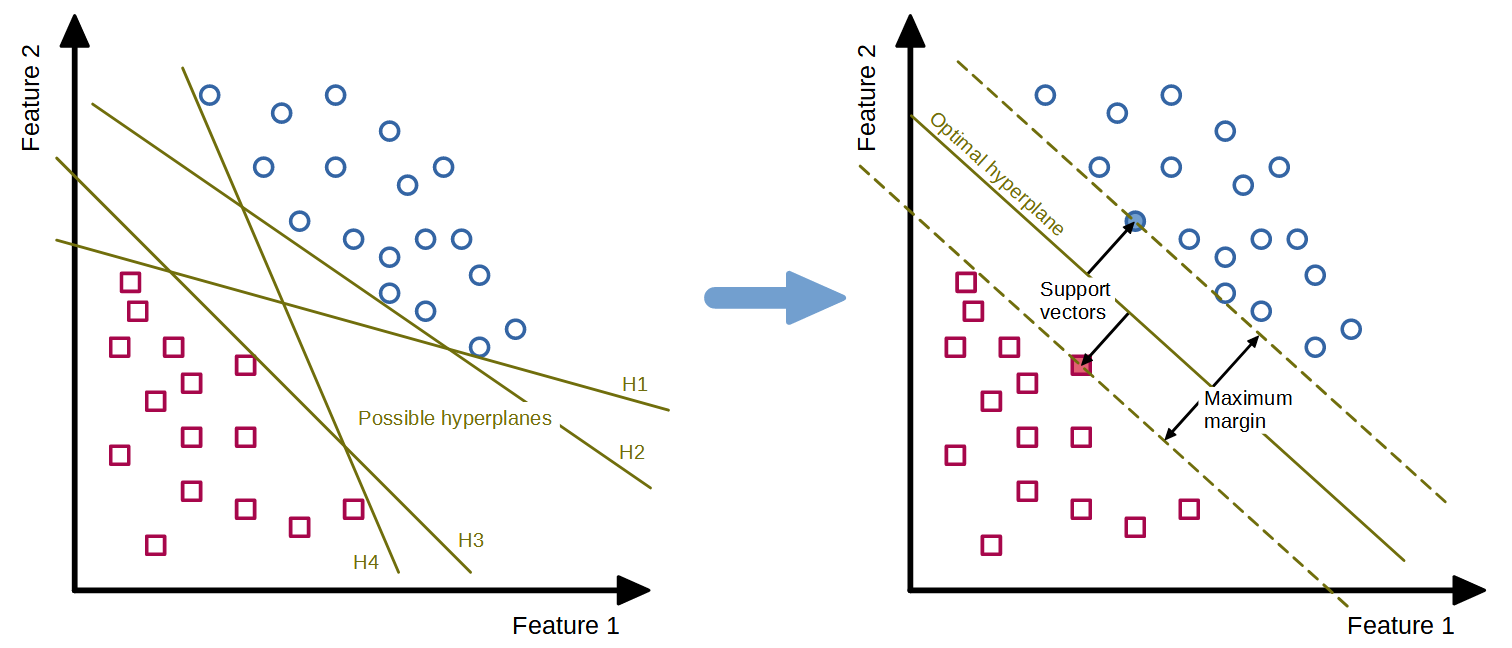
\includegraphics{images/SVC_operatingPrinciple.png}
\caption{Support Vectors Classifiers (SVC) separate the data points in
classes by finding the best hyperplane}
\end{figure}

    \hypertarget{split-the-dataset}{%
\subsection{Split the dataset}\label{split-the-dataset}}

In the next very important step, the dataset is split into \textbf{2
subsets}: a \textbf{training dataset} and a \textbf{test dataset}. As
the names suggest, the training dataset is used to train the ML
algorithm. The test data set is then used to check the quality of the
trained ML algorithm (here the \textbf{recognition rate}). For this
purpose, the \textbf{class labels} are \textbf{removed} from the
training data set - after all, these are to be predicted.

Typically, the \textbf{test dataset} should contain about \textbf{20\%}
of the entire dataset.

    \begin{tcolorbox}[breakable, size=fbox, boxrule=1pt, pad at break*=1mm,colback=cellbackground, colframe=cellborder]
\prompt{In}{incolor}{52}{\boxspacing}
\begin{Verbatim}[commandchars=\\\{\}]
\PY{k+kn}{from} \PY{n+nn}{sklearn}\PY{n+nn}{.}\PY{n+nn}{model\PYZus{}selection} \PY{k+kn}{import} \PY{n}{train\PYZus{}test\PYZus{}split}

\PY{n}{X} \PY{o}{=} \PY{n}{irisdata\PYZus{}df}\PY{o}{.}\PY{n}{drop}\PY{p}{(}\PY{l+s+s1}{\PYZsq{}}\PY{l+s+s1}{species}\PY{l+s+s1}{\PYZsq{}}\PY{p}{,} \PY{n}{axis}\PY{o}{=}\PY{l+m+mi}{1}\PY{p}{)}
\PY{n}{y} \PY{o}{=} \PY{n}{irisdata\PYZus{}df}\PY{p}{[}\PY{l+s+s1}{\PYZsq{}}\PY{l+s+s1}{species}\PY{l+s+s1}{\PYZsq{}}\PY{p}{]}

\PY{n}{X\PYZus{}train}\PY{p}{,} \PY{n}{X\PYZus{}test}\PY{p}{,} \PY{n}{y\PYZus{}train}\PY{p}{,} \PY{n}{y\PYZus{}test} \PY{o}{=} \PY{n}{train\PYZus{}test\PYZus{}split}\PY{p}{(}\PY{n}{X}\PY{p}{,} \PY{n}{y}\PY{p}{,} \PY{n}{test\PYZus{}size} \PY{o}{=} \PY{l+m+mf}{0.20}\PY{p}{)}
\end{Verbatim}
\end{tcolorbox}

    For training, do not use only the variables that correlate best with
each other, but all of them.

Otherwise, the result of the prediction would be significantly worse.
Maybe this is already an indication of \textbf{overfitting} of the ML
model.

    \begin{tcolorbox}[breakable, size=fbox, boxrule=1pt, pad at break*=1mm,colback=cellbackground, colframe=cellborder]
\prompt{In}{incolor}{38}{\boxspacing}
\begin{Verbatim}[commandchars=\\\{\}]
\PY{c+c1}{\PYZsh{} DO NOT USE THIS!!}
\PY{n}{X\PYZus{}train}\PY{p}{,} \PY{n}{X\PYZus{}test}\PY{p}{,} \PY{n}{y\PYZus{}train}\PY{p}{,} \PY{n}{y\PYZus{}test} \PY{o}{=} \PY{n}{train\PYZus{}test\PYZus{}split}\PY{p}{(}\PY{n}{X}\PY{p}{[}\PY{p}{[}\PY{l+s+s1}{\PYZsq{}}\PY{l+s+s1}{sepal\PYZus{}length}\PY{l+s+s1}{\PYZsq{}}\PY{p}{,} 
                                                       \PY{l+s+s1}{\PYZsq{}}\PY{l+s+s1}{sepal\PYZus{}width}\PY{l+s+s1}{\PYZsq{}}\PY{p}{]}\PY{p}{]}\PY{p}{,} 
                                                    \PY{n}{y}\PY{p}{,} \PY{n}{test\PYZus{}size} \PY{o}{=} \PY{l+m+mf}{0.20}\PY{p}{)}
\end{Verbatim}
\end{tcolorbox}

    \hypertarget{create-the-svm-model}{%
\subsection{Create the SVM model}\label{create-the-svm-model}}

In this step we create the SVC model and fit it to our training data.

    \begin{tcolorbox}[breakable, size=fbox, boxrule=1pt, pad at break*=1mm,colback=cellbackground, colframe=cellborder]
\prompt{In}{incolor}{53}{\boxspacing}
\begin{Verbatim}[commandchars=\\\{\}]
\PY{k+kn}{from} \PY{n+nn}{sklearn}\PY{n+nn}{.}\PY{n+nn}{svm} \PY{k+kn}{import} \PY{n}{SVC}
\PY{n}{classifier} \PY{o}{=} \PY{n}{SVC}\PY{p}{(}\PY{n}{kernel} \PY{o}{=} \PY{l+s+s1}{\PYZsq{}}\PY{l+s+s1}{linear}\PY{l+s+s1}{\PYZsq{}}\PY{p}{,} \PY{n}{random\PYZus{}state} \PY{o}{=} \PY{l+m+mi}{0}\PY{p}{)}

\PY{c+c1}{\PYZsh{} fit the model for the data}
\PY{n}{classifier}\PY{o}{.}\PY{n}{fit}\PY{p}{(}\PY{n}{X\PYZus{}train}\PY{p}{,} \PY{n}{y\PYZus{}train}\PY{p}{)}
\end{Verbatim}
\end{tcolorbox}

            \begin{tcolorbox}[breakable, size=fbox, boxrule=.5pt, pad at break*=1mm, opacityfill=0]
\prompt{Out}{outcolor}{53}{\boxspacing}
\begin{Verbatim}[commandchars=\\\{\}]
SVC(kernel='linear', random\_state=0)
\end{Verbatim}
\end{tcolorbox}
        
    \hypertarget{make-predictions}{%
\subsection{Make predictions}\label{make-predictions}}

    \begin{tcolorbox}[breakable, size=fbox, boxrule=1pt, pad at break*=1mm,colback=cellbackground, colframe=cellborder]
\prompt{In}{incolor}{54}{\boxspacing}
\begin{Verbatim}[commandchars=\\\{\}]
\PY{n}{y\PYZus{}pred} \PY{o}{=} \PY{n}{classifier}\PY{o}{.}\PY{n}{predict}\PY{p}{(}\PY{n}{X\PYZus{}test}\PY{p}{)}
\PY{c+c1}{\PYZsh{}X\PYZus{}test}
\end{Verbatim}
\end{tcolorbox}

    \hypertarget{step-4-evaluate-the-classification-results---metrics}{%
\section{STEP 4: Evaluate the classification results -
metrics}\label{step-4-evaluate-the-classification-results---metrics}}

And finally for checking the accuracy of the model, the
\textbf{confusion matrix} is used for the \textbf{cross validation}.

By using the function \texttt{sklearn.metrics.confusion\_matrix()} a
confusion matrix of the true digit values versus the predicted digit
values is plotted.

\hypertarget{textual-confusion-matrix}{%
\subsection{Textual confusion matrix}\label{textual-confusion-matrix}}

    \begin{tcolorbox}[breakable, size=fbox, boxrule=1pt, pad at break*=1mm,colback=cellbackground, colframe=cellborder]
\prompt{In}{incolor}{55}{\boxspacing}
\begin{Verbatim}[commandchars=\\\{\}]
\PY{n}{cm} \PY{o}{=} \PY{n}{metrics}\PY{o}{.}\PY{n}{confusion\PYZus{}matrix}\PY{p}{(}\PY{n}{y\PYZus{}test}\PY{p}{,} \PY{n}{y\PYZus{}pred}\PY{p}{)}
\PY{n+nb}{print}\PY{p}{(}\PY{n}{cm}\PY{p}{)}
\end{Verbatim}
\end{tcolorbox}

    \begin{Verbatim}[commandchars=\\\{\}]
[[14  0  0]
 [ 0  9  1]
 [ 0  0  6]]
    \end{Verbatim}

    \hypertarget{colored-confusion-matrix}{%
\subsection{Colored confusion matrix}\label{colored-confusion-matrix}}

The function \texttt{sklearn.metrics.ConfusionMatrixDisplay()} plots a
colored confusion matrix.

    \begin{tcolorbox}[breakable, size=fbox, boxrule=1pt, pad at break*=1mm,colback=cellbackground, colframe=cellborder]
\prompt{In}{incolor}{67}{\boxspacing}
\begin{Verbatim}[commandchars=\\\{\}]
\PY{n}{sns}\PY{o}{.}\PY{n}{set\PYZus{}style}\PY{p}{(}\PY{l+s+s2}{\PYZdq{}}\PY{l+s+s2}{white}\PY{l+s+s2}{\PYZdq{}}\PY{p}{)}

\PY{c+c1}{\PYZsh{} print colored confusion matrix}
\PY{n}{cm\PYZus{}colored} \PY{o}{=} \PY{n}{metrics}\PY{o}{.}\PY{n}{ConfusionMatrixDisplay}\PY{o}{.}\PY{n}{from\PYZus{}predictions}\PY{p}{(}\PY{n}{y\PYZus{}test}\PY{p}{,} \PY{n}{y\PYZus{}pred}\PY{p}{)}

\PY{c+c1}{\PYZsh{}cm\PYZus{}colored.figure\PYZus{}.suptitle(\PYZdq{}Confusion Matrix\PYZdq{})}
\PY{n}{cm\PYZus{}colored}\PY{o}{.}\PY{n}{figure\PYZus{}}\PY{o}{.}\PY{n}{set\PYZus{}figwidth}\PY{p}{(}\PY{l+m+mi}{8}\PY{p}{)}
\PY{n}{cm\PYZus{}colored}\PY{o}{.}\PY{n}{figure\PYZus{}}\PY{o}{.}\PY{n}{set\PYZus{}figheight}\PY{p}{(}\PY{l+m+mi}{7}\PY{p}{)}

\PY{n}{cm\PYZus{}colored}\PY{o}{.}\PY{n}{confusion\PYZus{}matrix}

\PY{c+c1}{\PYZsh{} save figure as PNG}
\PY{n}{plt}\PY{o}{.}\PY{n}{tight\PYZus{}layout}\PY{p}{(}\PY{p}{)}
\PY{n}{plt}\PY{o}{.}\PY{n}{savefig}\PY{p}{(}\PY{l+s+s1}{\PYZsq{}}\PY{l+s+s1}{images/confusion\PYZus{}matrix.png}\PY{l+s+s1}{\PYZsq{}}\PY{p}{,} \PY{n}{dpi}\PY{o}{=}\PY{l+m+mi}{150}\PY{p}{,} \PY{n}{pad\PYZus{}inches}\PY{o}{=}\PY{l+m+mi}{5}\PY{p}{)}
\PY{n}{plt}\PY{o}{.}\PY{n}{show}\PY{p}{(}\PY{p}{)}
\end{Verbatim}
\end{tcolorbox}

    \begin{figure}[h!]
        \begin{center}\adjustimage{max size={0.9\linewidth}{0.4\paperheight}}{SVM_Iris_parameter_tuning_files/SVM_Iris_parameter_tuning_87_0.png}\end{center}
        \caption{}
        \label{}
    \end{figure}
    
    \begin{tcolorbox}[breakable, size=fbox, boxrule=1pt, pad at break*=1mm,colback=cellbackground, colframe=cellborder]
\prompt{In}{incolor}{43}{\boxspacing}
\begin{Verbatim}[commandchars=\\\{\}]
\PY{k+kn}{from} \PY{n+nn}{sklearn}\PY{n+nn}{.}\PY{n+nn}{model\PYZus{}selection} \PY{k+kn}{import} \PY{n}{cross\PYZus{}val\PYZus{}score}

\PY{n}{accuracies} \PY{o}{=} \PY{n}{cross\PYZus{}val\PYZus{}score}\PY{p}{(}\PY{n}{estimator} \PY{o}{=} \PY{n}{classifier}\PY{p}{,} \PY{n}{X} \PY{o}{=} \PY{n}{X\PYZus{}train}\PY{p}{,} 
                             \PY{n}{y} \PY{o}{=} \PY{n}{y\PYZus{}train}\PY{p}{,} \PY{n}{cv} \PY{o}{=} \PY{l+m+mi}{10}\PY{p}{)}

\PY{n+nb}{print}\PY{p}{(}\PY{l+s+s2}{\PYZdq{}}\PY{l+s+s2}{Accuracy: }\PY{l+s+si}{\PYZob{}:.2f\PYZcb{}}\PY{l+s+s2}{ }\PY{l+s+s2}{\PYZpc{}}\PY{l+s+s2}{\PYZdq{}}\PY{o}{.}\PY{n}{format}\PY{p}{(}\PY{n}{accuracies}\PY{o}{.}\PY{n}{mean}\PY{p}{(}\PY{p}{)}\PY{o}{*}\PY{l+m+mi}{100}\PY{p}{)}\PY{p}{)}
\PY{n+nb}{print}\PY{p}{(}\PY{l+s+s2}{\PYZdq{}}\PY{l+s+s2}{Standard Deviation: }\PY{l+s+si}{\PYZob{}:.2f\PYZcb{}}\PY{l+s+s2}{ }\PY{l+s+s2}{\PYZpc{}}\PY{l+s+s2}{\PYZdq{}}\PY{o}{.}\PY{n}{format}\PY{p}{(}\PY{n}{accuracies}\PY{o}{.}\PY{n}{std}\PY{p}{(}\PY{p}{)}\PY{o}{*}\PY{l+m+mi}{100}\PY{p}{)}\PY{p}{)}
\end{Verbatim}
\end{tcolorbox}

    \begin{Verbatim}[commandchars=\\\{\}]
Accuracy: 79.17 \%
Standard Deviation: 6.72 \%
    \end{Verbatim}

    \hypertarget{step-5-select-svc-kernel-and-vary-parameters}{%
\section{STEP 5: Select SVC kernel and vary
parameters}\label{step-5-select-svc-kernel-and-vary-parameters}}

This section was inspired by
\href{https://medium.com/all-things-ai/in-depth-parameter-tuning-for-svc-758215394769}{In
Depth: Parameter tuning for SVC}

In this section, the 4 SVC parameters \texttt{kernel}, \texttt{gamma},
\texttt{C} and \texttt{degree} will be introduced one by one.
Furthermore, their influence on the classification result by varying
these single parameters will be shown.

\textbf{Disclaimer:} In order to show the effects of varying the
individual parameters in 2D graphs, only the best correlating variables
\texttt{petal\_length} and \texttt{petal\_width} are used to train the
SVC.

\hypertarget{prepare-dataset}{%
\subsection{Prepare dataset}\label{prepare-dataset}}

    \begin{tcolorbox}[breakable, size=fbox, boxrule=1pt, pad at break*=1mm,colback=cellbackground, colframe=cellborder]
\prompt{In}{incolor}{44}{\boxspacing}
\begin{Verbatim}[commandchars=\\\{\}]
\PY{c+c1}{\PYZsh{} import iris dataset again}
\PY{n}{irisdata\PYZus{}df} \PY{o}{=} \PY{n}{pd}\PY{o}{.}\PY{n}{read\PYZus{}csv}\PY{p}{(}\PY{l+s+s1}{\PYZsq{}}\PY{l+s+s1}{./datasets/IRIS\PYZus{}flower\PYZus{}dataset\PYZus{}kaggle.csv}\PY{l+s+s1}{\PYZsq{}}\PY{p}{)}

\PY{c+c1}{\PYZsh{} encode the class column from class strings to integer equivalents}
\PY{n}{irisdata\PYZus{}df\PYZus{}enc} \PY{o}{=} \PY{n}{irisdata\PYZus{}df}\PY{o}{.}\PY{n}{replace}\PY{p}{(}\PY{p}{\PYZob{}}\PY{l+s+s2}{\PYZdq{}}\PY{l+s+s2}{species}\PY{l+s+s2}{\PYZdq{}}\PY{p}{:}  \PY{p}{\PYZob{}}\PY{l+s+s2}{\PYZdq{}}\PY{l+s+s2}{Iris\PYZhy{}setosa}\PY{l+s+s2}{\PYZdq{}}\PY{p}{:}\PY{l+m+mi}{0}\PY{p}{,}
                                                    \PY{l+s+s2}{\PYZdq{}}\PY{l+s+s2}{Iris\PYZhy{}versicolor}\PY{l+s+s2}{\PYZdq{}}\PY{p}{:}\PY{l+m+mi}{1}\PY{p}{,} 
                                                    \PY{l+s+s2}{\PYZdq{}}\PY{l+s+s2}{Iris\PYZhy{}virginica}\PY{l+s+s2}{\PYZdq{}}\PY{p}{:}\PY{l+m+mi}{2}\PY{p}{\PYZcb{}}\PY{p}{\PYZcb{}}\PY{p}{)}
\PY{n}{irisdata\PYZus{}df\PYZus{}enc}
\end{Verbatim}
\end{tcolorbox}

            \begin{tcolorbox}[breakable, size=fbox, boxrule=.5pt, pad at break*=1mm, opacityfill=0]
\prompt{Out}{outcolor}{44}{\boxspacing}
\begin{Verbatim}[commandchars=\\\{\}]
     sepal\_length  sepal\_width  petal\_length  petal\_width  species
0             5.1          3.5           1.4          0.2        0
1             4.9          3.0           1.4          0.2        0
2             4.7          3.2           1.3          0.2        0
3             4.6          3.1           1.5          0.2        0
4             5.0          3.6           1.4          0.2        0
5             5.4          3.9           1.7          0.4        0
6             4.6          3.4           1.4          0.3        0
7             5.0          3.4           1.5          0.2        0
8             4.4          2.9           1.4          0.2        0
9             4.9          3.1           1.5          0.1        0
10            5.4          3.7           1.5          0.2        0
11            4.8          3.4           1.6          0.2        0
12            4.8          3.0           1.4          0.1        0
13            4.3          3.0           1.1          0.1        0
14            5.8          4.0           1.2          0.2        0
..            {\ldots}          {\ldots}           {\ldots}          {\ldots}      {\ldots}
135           7.7          3.0           6.1          2.3        2
136           6.3          3.4           5.6          2.4        2
137           6.4          3.1           5.5          1.8        2
138           6.0          3.0           4.8          1.8        2
139           6.9          3.1           5.4          2.1        2
140           6.7          3.1           5.6          2.4        2
141           6.9          3.1           5.1          2.3        2
142           5.8          2.7           5.1          1.9        2
143           6.8          3.2           5.9          2.3        2
144           6.7          3.3           5.7          2.5        2
145           6.7          3.0           5.2          2.3        2
146           6.3          2.5           5.0          1.9        2
147           6.5          3.0           5.2          2.0        2
148           6.2          3.4           5.4          2.3        2
149           5.9          3.0           5.1          1.8        2

[150 rows x 5 columns]
\end{Verbatim}
\end{tcolorbox}
        
    \begin{tcolorbox}[breakable, size=fbox, boxrule=1pt, pad at break*=1mm,colback=cellbackground, colframe=cellborder]
\prompt{In}{incolor}{45}{\boxspacing}
\begin{Verbatim}[commandchars=\\\{\}]
\PY{c+c1}{\PYZsh{} copy only 2 feature columns}
\PY{c+c1}{\PYZsh{} and convert pandas dataframe to numpy array}
\PY{n}{X} \PY{o}{=} \PY{n}{irisdata\PYZus{}df\PYZus{}enc}\PY{p}{[}\PY{p}{[}\PY{l+s+s1}{\PYZsq{}}\PY{l+s+s1}{petal\PYZus{}length}\PY{l+s+s1}{\PYZsq{}}\PY{p}{,} \PY{l+s+s1}{\PYZsq{}}\PY{l+s+s1}{petal\PYZus{}width}\PY{l+s+s1}{\PYZsq{}}\PY{p}{]}\PY{p}{]}\PY{o}{.}\PY{n}{to\PYZus{}numpy}\PY{p}{(}\PY{n}{copy}\PY{o}{=}\PY{k+kc}{True}\PY{p}{)}
\PY{c+c1}{\PYZsh{}X = irisdata\PYZus{}df\PYZus{}enc[[\PYZsq{}sepal\PYZus{}length\PYZsq{}, \PYZsq{}sepal\PYZus{}width\PYZsq{}]].to\PYZus{}numpy(copy=True)}
\PY{c+c1}{\PYZsh{}X}
\end{Verbatim}
\end{tcolorbox}

    \begin{tcolorbox}[breakable, size=fbox, boxrule=1pt, pad at break*=1mm,colback=cellbackground, colframe=cellborder]
\prompt{In}{incolor}{46}{\boxspacing}
\begin{Verbatim}[commandchars=\\\{\}]
\PY{c+c1}{\PYZsh{} convert pandas dataframe to numpy array}
\PY{c+c1}{\PYZsh{} and get a flat 1D copy of 2D numpy array}
\PY{n}{y} \PY{o}{=} \PY{n}{irisdata\PYZus{}df\PYZus{}enc}\PY{p}{[}\PY{p}{[}\PY{l+s+s1}{\PYZsq{}}\PY{l+s+s1}{species}\PY{l+s+s1}{\PYZsq{}}\PY{p}{]}\PY{p}{]}\PY{o}{.}\PY{n}{to\PYZus{}numpy}\PY{p}{(}\PY{n}{copy}\PY{o}{=}\PY{k+kc}{True}\PY{p}{)}\PY{o}{.}\PY{n}{flatten}\PY{p}{(}\PY{p}{)}
\PY{c+c1}{\PYZsh{}y}
\end{Verbatim}
\end{tcolorbox}

    \hypertarget{plotting-function}{%
\subsection{Plotting function}\label{plotting-function}}

This function helps to visualize the modifications by varying the
individual SVC parameters.

    \begin{tcolorbox}[breakable, size=fbox, boxrule=1pt, pad at break*=1mm,colback=cellbackground, colframe=cellborder]
\prompt{In}{incolor}{47}{\boxspacing}
\begin{Verbatim}[commandchars=\\\{\}]
\PY{k}{def} \PY{n+nf}{plotSVC}\PY{p}{(}\PY{n}{title}\PY{p}{,} \PY{n}{xlabel}\PY{p}{,} \PY{n}{ylabel}\PY{p}{)}\PY{p}{:}
    \PY{c+c1}{\PYZsh{} create a mesh to plot in}
    \PY{n}{x\PYZus{}min}\PY{p}{,} \PY{n}{x\PYZus{}max} \PY{o}{=} \PY{n}{X}\PY{p}{[}\PY{p}{:}\PY{p}{,} \PY{l+m+mi}{0}\PY{p}{]}\PY{o}{.}\PY{n}{min}\PY{p}{(}\PY{p}{)} \PY{o}{\PYZhy{}} \PY{l+m+mi}{1}\PY{p}{,} \PY{n}{X}\PY{p}{[}\PY{p}{:}\PY{p}{,} \PY{l+m+mi}{0}\PY{p}{]}\PY{o}{.}\PY{n}{max}\PY{p}{(}\PY{p}{)} \PY{o}{+} \PY{l+m+mi}{1}
    \PY{n}{y\PYZus{}min}\PY{p}{,} \PY{n}{y\PYZus{}max} \PY{o}{=} \PY{n}{X}\PY{p}{[}\PY{p}{:}\PY{p}{,} \PY{l+m+mi}{1}\PY{p}{]}\PY{o}{.}\PY{n}{min}\PY{p}{(}\PY{p}{)} \PY{o}{\PYZhy{}} \PY{l+m+mi}{1}\PY{p}{,} \PY{n}{X}\PY{p}{[}\PY{p}{:}\PY{p}{,} \PY{l+m+mi}{1}\PY{p}{]}\PY{o}{.}\PY{n}{max}\PY{p}{(}\PY{p}{)} \PY{o}{+} \PY{l+m+mi}{1}
    
    \PY{c+c1}{\PYZsh{} prevent division by zero}
    \PY{k}{if} \PY{n}{x\PYZus{}min} \PY{o}{==} \PY{l+m+mf}{0.0}\PY{p}{:}
        \PY{n}{x\PYZus{}min} \PY{o}{=} \PY{l+m+mf}{0.1}
    
    \PY{n}{h} \PY{o}{=} \PY{p}{(}\PY{n}{x\PYZus{}max} \PY{o}{/} \PY{n}{x\PYZus{}min}\PY{p}{)}\PY{o}{/}\PY{l+m+mi}{1000}
    \PY{n}{xx}\PY{p}{,} \PY{n}{yy} \PY{o}{=} \PY{n}{np}\PY{o}{.}\PY{n}{meshgrid}\PY{p}{(}\PY{n}{np}\PY{o}{.}\PY{n}{arange}\PY{p}{(}\PY{n}{x\PYZus{}min}\PY{p}{,} \PY{n}{x\PYZus{}max}\PY{p}{,} \PY{n}{h}\PY{p}{)}\PY{p}{,} \PY{n}{np}\PY{o}{.}\PY{n}{arange}\PY{p}{(}\PY{n}{y\PYZus{}min}\PY{p}{,} \PY{n}{y\PYZus{}max}\PY{p}{,} \PY{n}{h}\PY{p}{)}\PY{p}{)}
    
    \PY{n}{plt}\PY{o}{.}\PY{n}{subplot}\PY{p}{(}\PY{l+m+mi}{1}\PY{p}{,} \PY{l+m+mi}{1}\PY{p}{,} \PY{l+m+mi}{1}\PY{p}{)}
    \PY{n}{Z} \PY{o}{=} \PY{n}{svc}\PY{o}{.}\PY{n}{predict}\PY{p}{(}\PY{n}{np}\PY{o}{.}\PY{n}{c\PYZus{}}\PY{p}{[}\PY{n}{xx}\PY{o}{.}\PY{n}{ravel}\PY{p}{(}\PY{p}{)}\PY{p}{,} \PY{n}{yy}\PY{o}{.}\PY{n}{ravel}\PY{p}{(}\PY{p}{)}\PY{p}{]}\PY{p}{)}
    \PY{n}{Z} \PY{o}{=} \PY{n}{Z}\PY{o}{.}\PY{n}{reshape}\PY{p}{(}\PY{n}{xx}\PY{o}{.}\PY{n}{shape}\PY{p}{)}
    
    \PY{n}{plt}\PY{o}{.}\PY{n}{contourf}\PY{p}{(}\PY{n}{xx}\PY{p}{,} \PY{n}{yy}\PY{p}{,} \PY{n}{Z}\PY{p}{,} \PY{n}{cmap}\PY{o}{=}\PY{n}{plt}\PY{o}{.}\PY{n}{cm}\PY{o}{.}\PY{n}{Paired}\PY{p}{,} \PY{n}{alpha}\PY{o}{=}\PY{l+m+mf}{0.6}\PY{p}{)}
    \PY{n}{plt}\PY{o}{.}\PY{n}{scatter}\PY{p}{(}\PY{n}{X}\PY{p}{[}\PY{p}{:}\PY{p}{,} \PY{l+m+mi}{0}\PY{p}{]}\PY{p}{,} \PY{n}{X}\PY{p}{[}\PY{p}{:}\PY{p}{,} \PY{l+m+mi}{1}\PY{p}{]}\PY{p}{,} \PY{n}{c}\PY{o}{=}\PY{n}{y}\PY{p}{,} \PY{n}{cmap}\PY{o}{=}\PY{n}{plt}\PY{o}{.}\PY{n}{cm}\PY{o}{.}\PY{n}{Paired}\PY{p}{)}
    \PY{n}{plt}\PY{o}{.}\PY{n}{xlabel}\PY{p}{(}\PY{n}{xlabel}\PY{p}{)}
    \PY{n}{plt}\PY{o}{.}\PY{n}{ylabel}\PY{p}{(}\PY{n}{ylabel}\PY{p}{)}
    \PY{n}{plt}\PY{o}{.}\PY{n}{xlim}\PY{p}{(}\PY{n}{xx}\PY{o}{.}\PY{n}{min}\PY{p}{(}\PY{p}{)}\PY{p}{,} \PY{n}{xx}\PY{o}{.}\PY{n}{max}\PY{p}{(}\PY{p}{)}\PY{p}{)}
    \PY{n}{plt}\PY{o}{.}\PY{n}{title}\PY{p}{(}\PY{n}{title}\PY{p}{)}
    \PY{n}{plt}\PY{o}{.}\PY{n}{show}\PY{p}{(}\PY{p}{)}
\end{Verbatim}
\end{tcolorbox}

    \hypertarget{vary-kernel-parameter}{%
\subsection{\texorpdfstring{Vary \texttt{kernel}
parameter}{Vary kernel parameter}}\label{vary-kernel-parameter}}

The \texttt{kernel} parameter selects the type of hyperplane that is
used to separate the data. Using \texttt{linear}
(\href{https://en.wikipedia.org/wiki/Linear_classifier}{linear
classifier}) kernel will use a linear hyperplane (a line in the case of
2D data). The \texttt{rbf}
(\href{https://en.wikipedia.org/wiki/Radial_basis_function_kernel}{radial
basis function kernel}) and \texttt{poly}
(\href{https://en.wikipedia.org/wiki/Polynomial_kernel}{polynomial
kernel}) kernel use non linear hyperplanes.

    \begin{tcolorbox}[breakable, size=fbox, boxrule=1pt, pad at break*=1mm,colback=cellbackground, colframe=cellborder]
\prompt{In}{incolor}{48}{\boxspacing}
\begin{Verbatim}[commandchars=\\\{\}]
\PY{n}{kernels} \PY{o}{=} \PY{p}{[}\PY{l+s+s1}{\PYZsq{}}\PY{l+s+s1}{linear}\PY{l+s+s1}{\PYZsq{}}\PY{p}{,} \PY{l+s+s1}{\PYZsq{}}\PY{l+s+s1}{rbf}\PY{l+s+s1}{\PYZsq{}}\PY{p}{,} \PY{l+s+s1}{\PYZsq{}}\PY{l+s+s1}{poly}\PY{l+s+s1}{\PYZsq{}}\PY{p}{]}

\PY{n}{xlabel} \PY{o}{=} \PY{l+s+s1}{\PYZsq{}}\PY{l+s+s1}{Petal length}\PY{l+s+s1}{\PYZsq{}}
\PY{n}{ylabel} \PY{o}{=} \PY{l+s+s1}{\PYZsq{}}\PY{l+s+s1}{Petal width}\PY{l+s+s1}{\PYZsq{}}

\PY{k}{for} \PY{n}{kernel} \PY{o+ow}{in} \PY{n}{kernels}\PY{p}{:}
    \PY{n}{svc} \PY{o}{=} \PY{n}{svm}\PY{o}{.}\PY{n}{SVC}\PY{p}{(}\PY{n}{kernel}\PY{o}{=}\PY{n}{kernel}\PY{p}{)}\PY{o}{.}\PY{n}{fit}\PY{p}{(}\PY{n}{X}\PY{p}{,} \PY{n}{y}\PY{p}{)}
    \PY{n}{plotSVC}\PY{p}{(}\PY{l+s+s1}{\PYZsq{}}\PY{l+s+s1}{kernel = }\PY{l+s+s1}{\PYZsq{}} \PY{o}{+} \PY{n+nb}{str}\PY{p}{(}\PY{n}{kernel}\PY{p}{)}\PY{p}{,} \PY{n}{xlabel}\PY{p}{,} \PY{n}{ylabel}\PY{p}{)}
\end{Verbatim}
\end{tcolorbox}

    \begin{figure}[h!]
        \begin{center}\adjustimage{max size={0.9\linewidth}{0.4\paperheight}}{SVM_Iris_parameter_tuning_files/SVM_Iris_parameter_tuning_96_0.png}\end{center}
        \caption{}
        \label{}
    \end{figure}
    
    \begin{figure}[h!]
        \begin{center}\adjustimage{max size={0.9\linewidth}{0.4\paperheight}}{SVM_Iris_parameter_tuning_files/SVM_Iris_parameter_tuning_96_1.png}\end{center}
        \caption{}
        \label{}
    \end{figure}
    
    \begin{figure}[h!]
        \begin{center}\adjustimage{max size={0.9\linewidth}{0.4\paperheight}}{SVM_Iris_parameter_tuning_files/SVM_Iris_parameter_tuning_96_2.png}\end{center}
        \caption{}
        \label{}
    \end{figure}
    
    \hypertarget{vary-gamma-parameter}{%
\subsection{\texorpdfstring{Vary \texttt{gamma}
parameter}{Vary gamma parameter}}\label{vary-gamma-parameter}}

The \texttt{gamma} parameter is used for non linear hyperplanes. The
higher the \texttt{gamma} value it tries to exactly fit the training
data set.

As we can see, increasing \texttt{gamma} leads to \textbf{overfitting}
as the classifier tries to perfectly fit the training data.

    \begin{tcolorbox}[breakable, size=fbox, boxrule=1pt, pad at break*=1mm,colback=cellbackground, colframe=cellborder]
\prompt{In}{incolor}{49}{\boxspacing}
\begin{Verbatim}[commandchars=\\\{\}]
\PY{n}{gammas} \PY{o}{=} \PY{p}{[}\PY{l+m+mf}{0.1}\PY{p}{,} \PY{l+m+mi}{1}\PY{p}{,} \PY{l+m+mi}{10}\PY{p}{,} \PY{l+m+mi}{100}\PY{p}{,} \PY{l+m+mi}{200}\PY{p}{]}

\PY{n}{xlabel} \PY{o}{=} \PY{l+s+s1}{\PYZsq{}}\PY{l+s+s1}{Petal length}\PY{l+s+s1}{\PYZsq{}}
\PY{n}{ylabel} \PY{o}{=} \PY{l+s+s1}{\PYZsq{}}\PY{l+s+s1}{Petal width}\PY{l+s+s1}{\PYZsq{}}

\PY{k}{for} \PY{n}{gamma} \PY{o+ow}{in} \PY{n}{gammas}\PY{p}{:}
    \PY{n}{svc} \PY{o}{=} \PY{n}{svm}\PY{o}{.}\PY{n}{SVC}\PY{p}{(}\PY{n}{kernel}\PY{o}{=}\PY{l+s+s1}{\PYZsq{}}\PY{l+s+s1}{rbf}\PY{l+s+s1}{\PYZsq{}}\PY{p}{,} \PY{n}{gamma}\PY{o}{=}\PY{n}{gamma}\PY{p}{)}\PY{o}{.}\PY{n}{fit}\PY{p}{(}\PY{n}{X}\PY{p}{,} \PY{n}{y}\PY{p}{)}
    \PY{n}{plotSVC}\PY{p}{(}\PY{l+s+s1}{\PYZsq{}}\PY{l+s+s1}{gamma = }\PY{l+s+s1}{\PYZsq{}} \PY{o}{+} \PY{n+nb}{str}\PY{p}{(}\PY{n}{gamma}\PY{p}{)}\PY{p}{,} \PY{n}{xlabel}\PY{p}{,} \PY{n}{ylabel}\PY{p}{)}
\end{Verbatim}
\end{tcolorbox}

    \begin{figure}[h!]
        \begin{center}\adjustimage{max size={0.9\linewidth}{0.4\paperheight}}{SVM_Iris_parameter_tuning_files/SVM_Iris_parameter_tuning_98_0.png}\end{center}
        \caption{}
        \label{}
    \end{figure}
    
    \begin{figure}[h!]
        \begin{center}\adjustimage{max size={0.9\linewidth}{0.4\paperheight}}{SVM_Iris_parameter_tuning_files/SVM_Iris_parameter_tuning_98_1.png}\end{center}
        \caption{}
        \label{}
    \end{figure}
    
    \begin{figure}[h!]
        \begin{center}\adjustimage{max size={0.9\linewidth}{0.4\paperheight}}{SVM_Iris_parameter_tuning_files/SVM_Iris_parameter_tuning_98_2.png}\end{center}
        \caption{}
        \label{}
    \end{figure}
    
    \begin{figure}[h!]
        \begin{center}\adjustimage{max size={0.9\linewidth}{0.4\paperheight}}{SVM_Iris_parameter_tuning_files/SVM_Iris_parameter_tuning_98_3.png}\end{center}
        \caption{}
        \label{}
    \end{figure}
    
    \begin{figure}[h!]
        \begin{center}\adjustimage{max size={0.9\linewidth}{0.4\paperheight}}{SVM_Iris_parameter_tuning_files/SVM_Iris_parameter_tuning_98_4.png}\end{center}
        \caption{}
        \label{}
    \end{figure}
    
    \hypertarget{vary-c-parameter}{%
\subsection{\texorpdfstring{Vary \texttt{C}
parameter}{Vary C parameter}}\label{vary-c-parameter}}

The \texttt{C} parameter is the \textbf{penalty} of the error term. It
controls the trade off between smooth decision boundary and classifying
the training points correctly.

But be careful: to high \texttt{C} values may lead to
\textbf{overfitting} the training data.

    \begin{tcolorbox}[breakable, size=fbox, boxrule=1pt, pad at break*=1mm,colback=cellbackground, colframe=cellborder]
\prompt{In}{incolor}{50}{\boxspacing}
\begin{Verbatim}[commandchars=\\\{\}]
\PY{n}{cs} \PY{o}{=} \PY{p}{[}\PY{l+m+mf}{0.1}\PY{p}{,} \PY{l+m+mi}{1}\PY{p}{,} \PY{l+m+mi}{10}\PY{p}{,} \PY{l+m+mi}{100}\PY{p}{,} \PY{l+m+mi}{1000}\PY{p}{,} \PY{l+m+mi}{10000}\PY{p}{]}

\PY{n}{xlabel} \PY{o}{=} \PY{l+s+s1}{\PYZsq{}}\PY{l+s+s1}{Petal length}\PY{l+s+s1}{\PYZsq{}}
\PY{n}{ylabel} \PY{o}{=} \PY{l+s+s1}{\PYZsq{}}\PY{l+s+s1}{Petal width}\PY{l+s+s1}{\PYZsq{}}

\PY{k}{for} \PY{n}{c} \PY{o+ow}{in} \PY{n}{cs}\PY{p}{:}
    \PY{n}{svc} \PY{o}{=} \PY{n}{svm}\PY{o}{.}\PY{n}{SVC}\PY{p}{(}\PY{n}{kernel}\PY{o}{=}\PY{l+s+s1}{\PYZsq{}}\PY{l+s+s1}{rbf}\PY{l+s+s1}{\PYZsq{}}\PY{p}{,} \PY{n}{C}\PY{o}{=}\PY{n}{c}\PY{p}{)}\PY{o}{.}\PY{n}{fit}\PY{p}{(}\PY{n}{X}\PY{p}{,} \PY{n}{y}\PY{p}{)}
    \PY{n}{plotSVC}\PY{p}{(}\PY{l+s+s1}{\PYZsq{}}\PY{l+s+s1}{C = }\PY{l+s+s1}{\PYZsq{}} \PY{o}{+} \PY{n+nb}{str}\PY{p}{(}\PY{n}{c}\PY{p}{)}\PY{p}{,} \PY{n}{xlabel}\PY{p}{,} \PY{n}{ylabel}\PY{p}{)}
\end{Verbatim}
\end{tcolorbox}

    \begin{figure}[h!]
        \begin{center}\adjustimage{max size={0.9\linewidth}{0.4\paperheight}}{SVM_Iris_parameter_tuning_files/SVM_Iris_parameter_tuning_100_0.png}\end{center}
        \caption{}
        \label{}
    \end{figure}
    
    \begin{figure}[h!]
        \begin{center}\adjustimage{max size={0.9\linewidth}{0.4\paperheight}}{SVM_Iris_parameter_tuning_files/SVM_Iris_parameter_tuning_100_1.png}\end{center}
        \caption{}
        \label{}
    \end{figure}
    
    \begin{figure}[h!]
        \begin{center}\adjustimage{max size={0.9\linewidth}{0.4\paperheight}}{SVM_Iris_parameter_tuning_files/SVM_Iris_parameter_tuning_100_2.png}\end{center}
        \caption{}
        \label{}
    \end{figure}
    
    \begin{figure}[h!]
        \begin{center}\adjustimage{max size={0.9\linewidth}{0.4\paperheight}}{SVM_Iris_parameter_tuning_files/SVM_Iris_parameter_tuning_100_3.png}\end{center}
        \caption{}
        \label{}
    \end{figure}
    
    \begin{figure}[h!]
        \begin{center}\adjustimage{max size={0.9\linewidth}{0.4\paperheight}}{SVM_Iris_parameter_tuning_files/SVM_Iris_parameter_tuning_100_4.png}\end{center}
        \caption{}
        \label{}
    \end{figure}
    
    \begin{figure}[h!]
        \begin{center}\adjustimage{max size={0.9\linewidth}{0.4\paperheight}}{SVM_Iris_parameter_tuning_files/SVM_Iris_parameter_tuning_100_5.png}\end{center}
        \caption{}
        \label{}
    \end{figure}
    
    \hypertarget{vary-degree-parameter}{%
\subsection{\texorpdfstring{Vary \texttt{degree}
parameter}{Vary degree parameter}}\label{vary-degree-parameter}}

The \texttt{degree} parameter is used when the \texttt{kernel} is set to
\texttt{poly}. It's basically the \textbf{degree of the polynomial} used
to find the hyperplane to split the data.

Using \texttt{degree\ =\ 1} is the same as using a \texttt{linear}
kernel. Also, increasing this parameters leads to \textbf{higher
training times}.

    \begin{tcolorbox}[breakable, size=fbox, boxrule=1pt, pad at break*=1mm,colback=cellbackground, colframe=cellborder]
\prompt{In}{incolor}{51}{\boxspacing}
\begin{Verbatim}[commandchars=\\\{\}]
\PY{n}{degrees} \PY{o}{=} \PY{p}{[}\PY{l+m+mi}{1}\PY{p}{,} \PY{l+m+mi}{2}\PY{p}{,} \PY{l+m+mi}{3}\PY{p}{,} \PY{l+m+mi}{4}\PY{p}{,} \PY{l+m+mi}{5}\PY{p}{,} \PY{l+m+mi}{6}\PY{p}{,} \PY{l+m+mi}{7}\PY{p}{,} \PY{l+m+mi}{8}\PY{p}{,} \PY{l+m+mi}{9}\PY{p}{,} \PY{l+m+mi}{10}\PY{p}{]}

\PY{n}{xlabel} \PY{o}{=} \PY{l+s+s1}{\PYZsq{}}\PY{l+s+s1}{Petal length}\PY{l+s+s1}{\PYZsq{}}
\PY{n}{ylabel} \PY{o}{=} \PY{l+s+s1}{\PYZsq{}}\PY{l+s+s1}{Petal width}\PY{l+s+s1}{\PYZsq{}}

\PY{k}{for} \PY{n}{degree} \PY{o+ow}{in} \PY{n}{degrees}\PY{p}{:}
    \PY{n}{svc} \PY{o}{=} \PY{n}{svm}\PY{o}{.}\PY{n}{SVC}\PY{p}{(}\PY{n}{kernel}\PY{o}{=}\PY{l+s+s1}{\PYZsq{}}\PY{l+s+s1}{poly}\PY{l+s+s1}{\PYZsq{}}\PY{p}{,} \PY{n}{degree}\PY{o}{=}\PY{n}{degree}\PY{p}{)}\PY{o}{.}\PY{n}{fit}\PY{p}{(}\PY{n}{X}\PY{p}{,} \PY{n}{y}\PY{p}{)}
    \PY{n}{plotSVC}\PY{p}{(}\PY{l+s+s1}{\PYZsq{}}\PY{l+s+s1}{degree = }\PY{l+s+s1}{\PYZsq{}} \PY{o}{+} \PY{n+nb}{str}\PY{p}{(}\PY{n}{degree}\PY{p}{)}\PY{p}{,} \PY{n}{xlabel}\PY{p}{,} \PY{n}{ylabel}\PY{p}{)}
\end{Verbatim}
\end{tcolorbox}

    \begin{figure}[h!]
        \begin{center}\adjustimage{max size={0.9\linewidth}{0.4\paperheight}}{SVM_Iris_parameter_tuning_files/SVM_Iris_parameter_tuning_102_0.png}\end{center}
        \caption{}
        \label{}
    \end{figure}
    
    \begin{figure}[h!]
        \begin{center}\adjustimage{max size={0.9\linewidth}{0.4\paperheight}}{SVM_Iris_parameter_tuning_files/SVM_Iris_parameter_tuning_102_1.png}\end{center}
        \caption{}
        \label{}
    \end{figure}
    
    \begin{figure}[h!]
        \begin{center}\adjustimage{max size={0.9\linewidth}{0.4\paperheight}}{SVM_Iris_parameter_tuning_files/SVM_Iris_parameter_tuning_102_2.png}\end{center}
        \caption{}
        \label{}
    \end{figure}
    
    \begin{figure}[h!]
        \begin{center}\adjustimage{max size={0.9\linewidth}{0.4\paperheight}}{SVM_Iris_parameter_tuning_files/SVM_Iris_parameter_tuning_102_3.png}\end{center}
        \caption{}
        \label{}
    \end{figure}
    
    \begin{figure}[h!]
        \begin{center}\adjustimage{max size={0.9\linewidth}{0.4\paperheight}}{SVM_Iris_parameter_tuning_files/SVM_Iris_parameter_tuning_102_4.png}\end{center}
        \caption{}
        \label{}
    \end{figure}
    
    \begin{figure}[h!]
        \begin{center}\adjustimage{max size={0.9\linewidth}{0.4\paperheight}}{SVM_Iris_parameter_tuning_files/SVM_Iris_parameter_tuning_102_5.png}\end{center}
        \caption{}
        \label{}
    \end{figure}
    
    \begin{figure}[h!]
        \begin{center}\adjustimage{max size={0.9\linewidth}{0.4\paperheight}}{SVM_Iris_parameter_tuning_files/SVM_Iris_parameter_tuning_102_6.png}\end{center}
        \caption{}
        \label{}
    \end{figure}
    
    \begin{figure}[h!]
        \begin{center}\adjustimage{max size={0.9\linewidth}{0.4\paperheight}}{SVM_Iris_parameter_tuning_files/SVM_Iris_parameter_tuning_102_7.png}\end{center}
        \caption{}
        \label{}
    \end{figure}
    
    \begin{figure}[h!]
        \begin{center}\adjustimage{max size={0.9\linewidth}{0.4\paperheight}}{SVM_Iris_parameter_tuning_files/SVM_Iris_parameter_tuning_102_8.png}\end{center}
        \caption{}
        \label{}
    \end{figure}
    
    \begin{figure}[h!]
        \begin{center}\adjustimage{max size={0.9\linewidth}{0.4\paperheight}}{SVM_Iris_parameter_tuning_files/SVM_Iris_parameter_tuning_102_9.png}\end{center}
        \caption{}
        \label{}
    \end{figure}
    

    % Add a bibliography block to the postdoc
    
    
    
\end{document}
